%%%%%%%%%%%%%%%%%%%%%%%%%%%%%%%%%%%%%%%%%
% The Legrand Orange Book
% LaTeX Template
% Version 2.4 (26/09/2018)
%
% This template was downloaded from:
% http://www.LaTeXTemplates.com
%
% Original author:
% Mathias Legrand (legrand.mathias@gmail.com) with modifications by:
% Vel (vel@latextemplates.com)
%
% License:
% CC BY-NC-SA 3.0 (http://creativecommons.org/licenses/by-nc-sa/3.0/)
%
% Compiling this template:
% This template uses biber for its bibliography and makeindex for its index.
% When you first open the template, compile it from the command line with the 
% commands below to make sure your LaTeX distribution is configured correctly:
%
% 1) pdflatex main
% 2) makeindex main.idx -s StyleInd.ist
% 3) biber main
% 4) pdflatex main x 2
%
% After this, when you wish to update the bibliography/index use the appropriate
% command above and make sure to compile with pdflatex several times 
% afterwards to propagate your changes to the document.
%
% This template also uses a number of packages which may need to be
% updated to the newest versions for the template to compile. It is strongly
% recommended you update your LaTeX distribution if you have any
% compilation errors.
%
% Important note:
% Chapter heading images should have a 2:1 width:height ratio,
% e.g. 920px width and 460px height.
%
%%%%%%%%%%%%%%%%%%%%%%%%%%%%%%%%%%%%%%%%%

% arara: pdflatex: { shell: yes } 
% arara: biber
% arara: pdflatex: { shell: yes }
% arara: htlatex
% arara: clean: { files: [ main.aux, main.log] }

%----------------------------------------------------------------------------------------
%	PACKAGES AND OTHER DOCUMENT CONFIGURATIONS
%----------------------------------------------------------------------------------------

\documentclass[11pt,fleqn]{book} % Default font size and left-justified equations

%%%%%%%%%%%%%%%%%%%%%%%%%%%%%%%%%%%%%%%%%
% The Legrand Orange Book
% Structural Definitions File
% Version 2.1 (26/09/2018)
%
% Original author:
% Mathias Legrand (legrand.mathias@gmail.com) with modifications by:
% Vel (vel@latextemplates.com)
% 
% This file was downloaded from:
% http://www.LaTeXTemplates.com
%
% License:
% CC BY-NC-SA 3.0 (http://creativecommons.org/licenses/by-nc-sa/3.0/)
%
%%%%%%%%%%%%%%%%%%%%%%%%%%%%%%%%%%%%%%%%%

%----------------------------------------------------------------------------------------
%	VARIOUS REQUIRED PACKAGES AND CONFIGURATIONS
%----------------------------------------------------------------------------------------
\usepackage{placeins}
\usepackage{graphicx} % Required for including pictures
\graphicspath{{Pictures/}} % Specifies the directory where pictures are stored

\usepackage{lipsum} % Inserts dummy text

\usepackage{tikz} % Required for drawing custom shapes

\usepackage[spanish]{babel} % English language/hyphenation

\usepackage{enumitem} % Customize lists
\setlist{nolistsep} % Reduce spacing between bullet points and numbered lists

\usepackage{booktabs} % Required for nicer horizontal rules in tables

\usepackage{xcolor} % Required for specifying colors by name

\usepackage[parfill]{parskip}
\usepackage{makecell}
\usepackage[]{xcolor}

\renewcommand\theadalign{bc}
\renewcommand\theadfont{\bfseries}
\renewcommand\theadgape{\Gape[4pt]}
\renewcommand\cellgape{\Gape[4pt]}

\definecolor{ocre}{RGB}{78,137,174} % Define the orange color used for highlighting throughout the book

%----------------------------------------------------------------------------------------
%	MARGINS
%----------------------------------------------------------------------------------------

\usepackage{geometry} % Required for adjusting page dimensions and margins

\geometry{
	paper=a4paper, % Paper size, change to letterpaper for US letter size
	top=3cm, % Top margin
	bottom=3cm, % Bottom margin
	left=3cm, % Left margin
	right=3cm, % Right margin
	headheight=14pt, % Header height
	footskip=1.4cm, % Space from the bottom margin to the baseline of the footer
	headsep=10pt, % Space from the top margin to the baseline of the header
	%showframe, % Uncomment to show how the type block is set on the page
}

%----------------------------------------------------------------------------------------
%	FONTS
%----------------------------------------------------------------------------------------

\usepackage{avant} % Use the Avantgarde font for headings
%\usepackage{times} % Use the Times font for headings
\usepackage{mathptmx} % Use the Adobe Times Roman as the default text font together with math symbols from the Sym­bol, Chancery and Com­puter Modern fonts
\usepackage{mathtools}
\usepackage{microtype} % Slightly tweak font spacing for aesthetics
\usepackage[utf8]{inputenc} % Required for including letters with accents
\usepackage[T1]{fontenc} % Use 8-bit encoding that has 256 glyphs
\setcounter{MaxMatrixCols}{13}
%----------------------------------------------------------------------------------------
%	BIBLIOGRAPHY AND INDEX
%----------------------------------------------------------------------------------------

\usepackage[style=numeric,citestyle=numeric,sorting=nyt,sortcites=true,autopunct=true,babel=hyphen,hyperref=true,abbreviate=false,backref=true,backend=biber]{biblatex}
\addbibresource{./bibliography.bib} % BibTeX bibliography file
\defbibheading{bibempty}{}

\usepackage{calc} % For simpler calculation - used for spacing the index letter headings correctly
\usepackage{makeidx} % Required to make an index
\makeindex % Tells LaTeX to create the files required for indexing

%----------------------------------------------------------------------------------------
%	MAIN TABLE OF CONTENTS
%----------------------------------------------------------------------------------------

\usepackage{titletoc} % Required for manipulating the table of contents

\contentsmargin{0cm} % Removes the default margin

% Part text styling (this is mostly taken care of in the PART HEADINGS section of this file)
\titlecontents{part}
	[0cm] % Left indentation
	{\addvspace{20pt}\bfseries} % Spacing and font options for parts
	{}
	{}
	{}

% Chapter text styling
\titlecontents{chapter}
	[1.25cm] % Left indentation
	{\addvspace{12pt}\large\sffamily\bfseries} % Spacing and font options for chapters
	{\color{ocre!60}\contentslabel[\Large\thecontentslabel]{1.25cm}\color{ocre}} % Formatting of numbered sections of this type
	{\color{ocre}} % Formatting of numberless sections of this type
	{\color{ocre!60}\normalsize\;\titlerule*[.5pc]{.}\;\thecontentspage} % Formatting of the filler to the right of the heading and the page number

% Section text styling
\titlecontents{section}
	[1.25cm] % Left indentation
	{\addvspace{3pt}\sffamily\bfseries} % Spacing and font options for sections
	{\contentslabel[\thecontentslabel]{1.25cm}} % Formatting of numbered sections of this type
	{} % Formatting of numberless sections of this type
	{\hfill\color{black}\thecontentspage} % Formatting of the filler to the right of the heading and the page number

% Subsection text styling
\titlecontents{subsection}
	[1.25cm] % Left indentation
	{\addvspace{1pt}\sffamily\small} % Spacing and font options for subsections
	{\contentslabel[\thecontentslabel]{1.25cm}} % Formatting of numbered sections of this type
	{} % Formatting of numberless sections of this type
	{\ \titlerule*[.5pc]{.}\;\thecontentspage} % Formatting of the filler to the right of the heading and the page number

% Figure text styling
\titlecontents{figure}
	[1.25cm] % Left indentation
	{\addvspace{1pt}\sffamily\small} % Spacing and font options for figures
	{\thecontentslabel\hspace*{1em}} % Formatting of numbered sections of this type
	{} % Formatting of numberless sections of this type
	{\ \titlerule*[.5pc]{.}\;\thecontentspage} % Formatting of the filler to the right of the heading and the page number

% Table text styling
\titlecontents{table}
	[1.25cm] % Left indentation
	{\addvspace{1pt}\sffamily\small} % Spacing and font options for tables
	{\thecontentslabel\hspace*{1em}} % Formatting of numbered sections of this type
	{} % Formatting of numberless sections of this type
	{\ \titlerule*[.5pc]{.}\;\thecontentspage} % Formatting of the filler to the right of the heading and the page number

%----------------------------------------------------------------------------------------
%	MINI TABLE OF CONTENTS IN PART HEADS
%----------------------------------------------------------------------------------------

% Chapter text styling
\titlecontents{lchapter}
	[0em] % Left indentation
	{\addvspace{15pt}\large\sffamily\bfseries} % Spacing and font options for chapters
	{\color{ocre}\contentslabel[\Large\thecontentslabel]{1.25cm}\color{ocre}} % Chapter number
	{}  
	{\color{ocre}\normalsize\sffamily\bfseries\;\titlerule*[.5pc]{.}\;\thecontentspage} % Page number

% Section text styling
\titlecontents{lsection}
	[0em] % Left indentation
	{\sffamily\small} % Spacing and font options for sections
	{\contentslabel[\thecontentslabel]{1.25cm}} % Section number
	{}
	{}

% Subsection text styling (note these aren't shown by default, display them by searchings this file for tocdepth and reading the commented text)
\titlecontents{lsubsection}
	[.5em] % Left indentation
	{\sffamily\footnotesize} % Spacing and font options for subsections
	{\contentslabel[\thecontentslabel]{1.25cm}}
	{}
	{}

%----------------------------------------------------------------------------------------
%	HEADERS AND FOOTERS
%----------------------------------------------------------------------------------------

\usepackage{fancyhdr} % Required for header and footer configuration

\pagestyle{fancy} % Enable the custom headers and footers

\renewcommand{\chaptermark}[1]{\markboth{\sffamily\normalsize\bfseries\chaptername\ \thechapter.\ #1}{}} % Styling for the current chapter in the header
\renewcommand{\sectionmark}[1]{\markright{\sffamily\normalsize\thesection\hspace{5pt}#1}{}} % Styling for the current section in the header

\fancyhf{} % Clear default headers and footers
\fancyhead[LE,RO]{\sffamily\normalsize\thepage} % Styling for the page number in the header
\fancyhead[LO]{\rightmark} % Print the nearest section name on the left side of odd pages
\fancyhead[RE]{\leftmark} % Print the current chapter name on the right side of even pages
%\fancyfoot[C]{\thepage} % Uncomment to include a footer

\renewcommand{\headrulewidth}{0.5pt} % Thickness of the rule under the header

\fancypagestyle{plain}{% Style for when a plain pagestyle is specified
	\fancyhead{}\renewcommand{\headrulewidth}{0pt}%
}

% Removes the header from odd empty pages at the end of chapters
\makeatletter
\renewcommand{\cleardoublepage}{
\clearpage\ifodd\c@page\else
\hbox{}
\vspace*{\fill}
\thispagestyle{empty}
\newpage
\fi}

%----------------------------------------------------------------------------------------
%	THEOREM STYLES
%----------------------------------------------------------------------------------------

\usepackage{amsmath,amsfonts,amssymb,amsthm} % For math equations, theorems, symbols, etc

\newcommand{\intoo}[2]{\mathopen{]}#1\,;#2\mathclose{[}}
\newcommand{\ud}{\mathop{\mathrm{{}d}}\mathopen{}}
\newcommand{\intff}[2]{\mathopen{[}#1\,;#2\mathclose{]}}
\renewcommand{\qedsymbol}{$\blacksquare$}
\newtheorem{notation}{Notation}[chapter]

% Boxed/framed environments
\newtheoremstyle{ocrenumbox}% Theorem style name
{0pt}% Space above
{0pt}% Space below
{\normalfont}% Body font
{}% Indent amount
{\small\bf\sffamily\color{ocre}}% Theorem head font
{\;}% Punctuation after theorem head
{0.25em}% Space after theorem head
{\small\sffamily\color{ocre}\thmname{#1}\nobreakspace\thmnumber{\@ifnotempty{#1}{}\@upn{#2}}% Theorem text (e.g. Theorem 2.1)
\thmnote{\nobreakspace\the\thm@notefont\sffamily\bfseries\color{black}---\nobreakspace#3.}} % Optional theorem note

\newtheoremstyle{blacknumex}% Theorem style name
{5pt}% Space above
{5pt}% Space below
{\normalfont}% Body font
{} % Indent amount
{\small\bf\sffamily}% Theorem head font
{\;}% Punctuation after theorem head
{0.25em}% Space after theorem head
{\small\sffamily{\tiny\ensuremath{\blacksquare}}\nobreakspace\thmname{#1}\nobreakspace\thmnumber{\@ifnotempty{#1}{}\@upn{#2}}% Theorem text (e.g. Theorem 2.1)
\thmnote{\nobreakspace\the\thm@notefont\sffamily\bfseries---\nobreakspace#3.}}% Optional theorem note

\newtheoremstyle{blacknumbox} % Theorem style name
{0pt}% Space above
{0pt}% Space below
{\normalfont}% Body font
{}% Indent amount
{\small\bf\sffamily}% Theorem head font
{\;}% Punctuation after theorem head
{0.25em}% Space after theorem head
{\small\sffamily\thmname{#1}\nobreakspace\thmnumber{\@ifnotempty{#1}{}\@upn{#2}}% Theorem text (e.g. Theorem 2.1)
\thmnote{\nobreakspace\the\thm@notefont\sffamily\bfseries---\nobreakspace#3.}}% Optional theorem note

% Non-boxed/non-framed environments
\newtheoremstyle{ocrenum}% Theorem style name
{5pt}% Space above
{5pt}% Space below
{\normalfont}% Body font
{}% Indent amount
{\small\bf\sffamily\color{ocre}}% Theorem head font
{\;}% Punctuation after theorem head
{0.25em}% Space after theorem head
{\small\sffamily\color{ocre}\thmname{#1}\nobreakspace\thmnumber{\@ifnotempty{#1}{}\@upn{#2}}% Theorem text (e.g. Theorem 2.1)
\thmnote{\nobreakspace\the\thm@notefont\sffamily\bfseries\color{black}---\nobreakspace#3.}} % Optional theorem note
\makeatother

% Defines the theorem text style for each type of theorem to one of the three styles above
\newcounter{dummy} 
\numberwithin{dummy}{section}
\theoremstyle{ocrenumbox}
\newtheorem{theoremeT}[dummy]{Theorem}
\newtheorem{problem}{Problem}[chapter]
\newtheorem{exerciseT}{Exercise}[chapter]
\theoremstyle{blacknumex}
\newtheorem{exampleT}{Example}[chapter]
\theoremstyle{blacknumbox}
\newtheorem{vocabulary}{Vocabulary}[chapter]
\newtheorem{definitionT}{Definition}[section]
\newtheorem{corollaryT}[dummy]{Corollary}
\theoremstyle{ocrenum}
\newtheorem{proposition}[dummy]{Proposition}

%----------------------------------------------------------------------------------------
%	DEFINITION OF COLORED BOXES
%----------------------------------------------------------------------------------------

\RequirePackage[framemethod=default]{mdframed} % Required for creating the theorem, definition, exercise and corollary boxes

% Theorem box
\newmdenv[skipabove=7pt,
skipbelow=7pt,
backgroundcolor=black!5,
linecolor=ocre,
innerleftmargin=5pt,
innerrightmargin=5pt,
innertopmargin=5pt,
leftmargin=0cm,
rightmargin=0cm,
innerbottommargin=5pt]{tBox}

% Exercise box	  
\newmdenv[skipabove=7pt,
skipbelow=7pt,
rightline=false,
leftline=true,
topline=false,
bottomline=false,
backgroundcolor=ocre!10,
linecolor=ocre,
innerleftmargin=5pt,
innerrightmargin=5pt,
innertopmargin=5pt,
innerbottommargin=5pt,
leftmargin=0cm,
rightmargin=0cm,
linewidth=4pt]{eBox}	

% Definition box
\newmdenv[skipabove=7pt,
skipbelow=7pt,
rightline=false,
leftline=true,
topline=false,
bottomline=false,
linecolor=ocre,
innerleftmargin=5pt,
innerrightmargin=5pt,
innertopmargin=0pt,
leftmargin=0cm,
rightmargin=0cm,
linewidth=4pt,
innerbottommargin=0pt]{dBox}	

% Corollary box
\newmdenv[skipabove=7pt,
skipbelow=7pt,
rightline=false,
leftline=true,
topline=false,
bottomline=false,
linecolor=gray,
backgroundcolor=black!5,
innerleftmargin=5pt,
innerrightmargin=5pt,
innertopmargin=5pt,
leftmargin=0cm,
rightmargin=0cm,
linewidth=4pt,
innerbottommargin=5pt]{cBox}

% Creates an environment for each type of theorem and assigns it a theorem text style from the "Theorem Styles" section above and a colored box from above
\newenvironment{theorem}{\begin{tBox}\begin{theoremeT}}{\end{theoremeT}\end{tBox}}
\newenvironment{exercise}{\begin{eBox}\begin{exerciseT}}{\hfill{\color{ocre}\tiny\ensuremath{\blacksquare}}\end{exerciseT}\end{eBox}}				  
\newenvironment{definition}{\begin{dBox}\begin{definitionT}}{\end{definitionT}\end{dBox}}	
\newenvironment{example}{\begin{exampleT}}{\hfill{\tiny\ensuremath{\blacksquare}}\end{exampleT}}		
\newenvironment{corollary}{\begin{cBox}\begin{corollaryT}}{\end{corollaryT}\end{cBox}}	

%----------------------------------------------------------------------------------------
%	REMARK ENVIRONMENT
%----------------------------------------------------------------------------------------

\newenvironment{remark}{\par\vspace{10pt}\small % Vertical white space above the remark and smaller font size
\begin{list}{}{
\leftmargin=35pt % Indentation on the left
\rightmargin=25pt}\item\ignorespaces % Indentation on the right
\makebox[-2.5pt]{\begin{tikzpicture}[overlay]
\node[draw=ocre!60,line width=1pt,circle,fill=ocre!25,font=\sffamily\bfseries,inner sep=2pt,outer sep=0pt] at (-15pt,0pt){\textcolor{ocre}{R}};\end{tikzpicture}} % Orange R in a circle
\advance\baselineskip -1pt}{\end{list}\vskip5pt} % Tighter line spacing and white space after remark

%----------------------------------------------------------------------------------------
%	SECTION NUMBERING IN THE MARGIN
%----------------------------------------------------------------------------------------

\makeatletter
\renewcommand{\@seccntformat}[1]{\llap{\textcolor{ocre}{\csname the#1\endcsname}\hspace{1em}}}                    
\renewcommand{\section}{\@startsection{section}{1}{\z@}
{-4ex \@plus -1ex \@minus -.4ex}
{1ex \@plus.2ex }
{\normalfont\large\sffamily\bfseries}}
\renewcommand{\subsection}{\@startsection {subsection}{2}{\z@}
{-3ex \@plus -0.1ex \@minus -.4ex}
{0.5ex \@plus.2ex }
{\normalfont\sffamily\bfseries}}
\renewcommand{\subsubsection}{\@startsection {subsubsection}{3}{\z@}
{-2ex \@plus -0.1ex \@minus -.2ex}
{.2ex \@plus.2ex }
{\normalfont\small\sffamily\bfseries}}                        
\renewcommand\paragraph{\@startsection{paragraph}{4}{\z@}
{-2ex \@plus-.2ex \@minus .2ex}
{.1ex}
{\normalfont\small\sffamily\bfseries}}

%----------------------------------------------------------------------------------------
%	PART HEADINGS
%----------------------------------------------------------------------------------------

% Numbered part in the table of contents
\newcommand{\@mypartnumtocformat}[2]{%
	\setlength\fboxsep{0pt}%
	\noindent\colorbox{ocre!20}{\strut\parbox[c][.7cm]{\ecart}{\color{ocre!70}\Large\sffamily\bfseries\centering#1}}\hskip\esp\colorbox{ocre!40}{\strut\parbox[c][.7cm]{\linewidth-\ecart-\esp}{\Large\sffamily\centering#2}}%
}

% Unnumbered part in the table of contents
\newcommand{\@myparttocformat}[1]{%
	\setlength\fboxsep{0pt}%
	\noindent\colorbox{ocre!40}{\strut\parbox[c][.7cm]{\linewidth}{\Large\sffamily\centering#1}}%
}

\newlength\esp
\setlength\esp{4pt}
\newlength\ecart
\setlength\ecart{1.2cm-\esp}
\newcommand{\thepartimage}{}%
\newcommand{\partimage}[1]{\renewcommand{\thepartimage}{#1}}%
\def\@part[#1]#2{%
\ifnum \c@secnumdepth >-2\relax%
\refstepcounter{part}%
\addcontentsline{toc}{part}{\texorpdfstring{\protect\@mypartnumtocformat{\thepart}{#1}}{\partname~\thepart\ ---\ #1}}
\else%
\addcontentsline{toc}{part}{\texorpdfstring{\protect\@myparttocformat{#1}}{#1}}%
\fi%
\startcontents%
\markboth{}{}%
{\thispagestyle{empty}%
\begin{tikzpicture}[remember picture,overlay]%
\node at (current page.north west){\begin{tikzpicture}[remember picture,overlay]%	
\fill[ocre!20](0cm,0cm) rectangle (\paperwidth,-\paperheight);
\node[anchor=north] at (4cm,-3.25cm){\color{ocre!40}\fontsize{220}{100}\sffamily\bfseries\thepart}; 
\node[anchor=south east] at (\paperwidth-1cm,-\paperheight+1cm){\parbox[t][][t]{8.5cm}{
\printcontents{l}{0}{\setcounter{tocdepth}{1}}% The depth to which the Part mini table of contents displays headings; 0 for chapters only, 1 for chapters and sections and 2 for chapters, sections and subsections
}};
\node[anchor=north east] at (\paperwidth-1.5cm,-3.25cm){\parbox[t][][t]{15cm}{\strut\raggedleft\color{white}\fontsize{30}{30}\sffamily\bfseries#2}};
\end{tikzpicture}};
\end{tikzpicture}}%
\@endpart}
\def\@spart#1{%
\startcontents%
\phantomsection
{\thispagestyle{empty}%
\begin{tikzpicture}[remember picture,overlay]%
\node at (current page.north west){\begin{tikzpicture}[remember picture,overlay]%	
\fill[ocre!20](0cm,0cm) rectangle (\paperwidth,-\paperheight);
\node[anchor=north east] at (\paperwidth-1.5cm,-3.25cm){\parbox[t][][t]{15cm}{\strut\raggedleft\color{white}\fontsize{30}{30}\sffamily\bfseries#1}};
\end{tikzpicture}};
\end{tikzpicture}}
\addcontentsline{toc}{part}{\texorpdfstring{%
\setlength\fboxsep{0pt}%
\noindent\protect\colorbox{ocre!40}{\strut\protect\parbox[c][.7cm]{\linewidth}{\Large\sffamily\protect\centering #1\quad\mbox{}}}}{#1}}%
\@endpart}
\def\@endpart{\vfil\newpage
\if@twoside
\if@openright
\null
\thispagestyle{empty}%
\newpage
\fi
\fi
\if@tempswa
\twocolumn
\fi}

%----------------------------------------------------------------------------------------
%	CHAPTER HEADINGS
%----------------------------------------------------------------------------------------

% A switch to conditionally include a picture, implemented by Christian Hupfer
\newif\ifusechapterimage
\usechapterimagetrue
\newcommand{\thechapterimage}{}%
\newcommand{\chapterimage}[1]{\ifusechapterimage\renewcommand{\thechapterimage}{#1}\fi}%
\newcommand{\autodot}{.}
\def\@makechapterhead#1{%
{\parindent \z@ \raggedright \normalfont
\ifnum \c@secnumdepth >\m@ne
\if@mainmatter
\begin{tikzpicture}[remember picture,overlay]
\node at (current page.north west)
{\begin{tikzpicture}[remember picture,overlay]
\node[anchor=north west,inner sep=0pt] at (0,0) {\ifusechapterimage\includegraphics[width=\paperwidth]{\thechapterimage}\fi};
\draw[anchor=west] (\Gm@lmargin,-9cm) node [line width=2pt,rounded corners=15pt,draw=ocre,fill=white,fill opacity=0.5,inner sep=15pt]{\strut\makebox[22cm]{}};
\draw[anchor=west] (\Gm@lmargin+.3cm,-9cm) node {\huge\sffamily\bfseries\color{black}\thechapter\autodot~#1\strut};
\end{tikzpicture}};
\end{tikzpicture}
\else
\begin{tikzpicture}[remember picture,overlay]
\node at (current page.north west)
{\begin{tikzpicture}[remember picture,overlay]
\node[anchor=north west,inner sep=0pt] at (0,0) {\ifusechapterimage\includegraphics[width=\paperwidth]{\thechapterimage}\fi};
\draw[anchor=west] (\Gm@lmargin,-9cm) node [line width=2pt,rounded corners=15pt,draw=ocre,fill=white,fill opacity=0.5,inner sep=15pt]{\strut\makebox[22cm]{}};
\draw[anchor=west] (\Gm@lmargin+.3cm,-9cm) node {\huge\sffamily\bfseries\color{black}#1\strut};
\end{tikzpicture}};
\end{tikzpicture}
\fi\fi\par\vspace*{270\p@}}}

%-------------------------------------------

\def\@makeschapterhead#1{%
\begin{tikzpicture}[remember picture,overlay]
\node at (current page.north west)
{\begin{tikzpicture}[remember picture,overlay]
\node[anchor=north west,inner sep=0pt] at (0,0) {\ifusechapterimage\includegraphics[width=\paperwidth]{\thechapterimage}\fi};
\draw[anchor=west] (\Gm@lmargin,-9cm) node [line width=2pt,rounded corners=15pt,draw=ocre,fill=white,fill opacity=0.5,inner sep=15pt]{\strut\makebox[22cm]{}};
\draw[anchor=west] (\Gm@lmargin+.3cm,-9cm) node {\huge\sffamily\bfseries\color{black}#1\strut};
\end{tikzpicture}};
\end{tikzpicture}
\par\vspace*{270\p@}}
\makeatother

%----------------------------------------------------------------------------------------
%	LINKS
%----------------------------------------------------------------------------------------

\usepackage{hyperref}
\hypersetup{hidelinks,backref=true,pagebackref=true,hyperindex=true,colorlinks=false,breaklinks=true,urlcolor=ocre,bookmarks=true,bookmarksopen=false}

\usepackage{bookmark}
\bookmarksetup{
open,
numbered,
addtohook={%
\ifnum\bookmarkget{level}=0 % chapter
\bookmarksetup{bold}%
\fi
\ifnum\bookmarkget{level}=-1 % part
\bookmarksetup{color=ocre,bold}%
\fi
}
}
 % Insert the commands.tex file which contains the majority of the structure behind the template

%\hypersetup{pdftitle={Title},pdfauthor={Author}} % Uncomment and fill out to include PDF metadata for the author and title of the book

%----------------------------------------------------------------------------------------
\usepackage[ruled,longend,noend]{algorithm2e}
\newcommand\mycommfont[1]{\footnotesize\ttfamily\textcolor{blue}{#1}}
\SetCommentSty{mycommfont}

\begin{document}

%----------------------------------------------------------------------------------------
%	TITLE PAGE
%----------------------------------------------------------------------------------------

\begingroup
\thispagestyle{empty} % Suppress headers and footers on the title page
\begin{tikzpicture}[remember picture,overlay]
\node[inner sep=0pt] (background) at (current page.center) {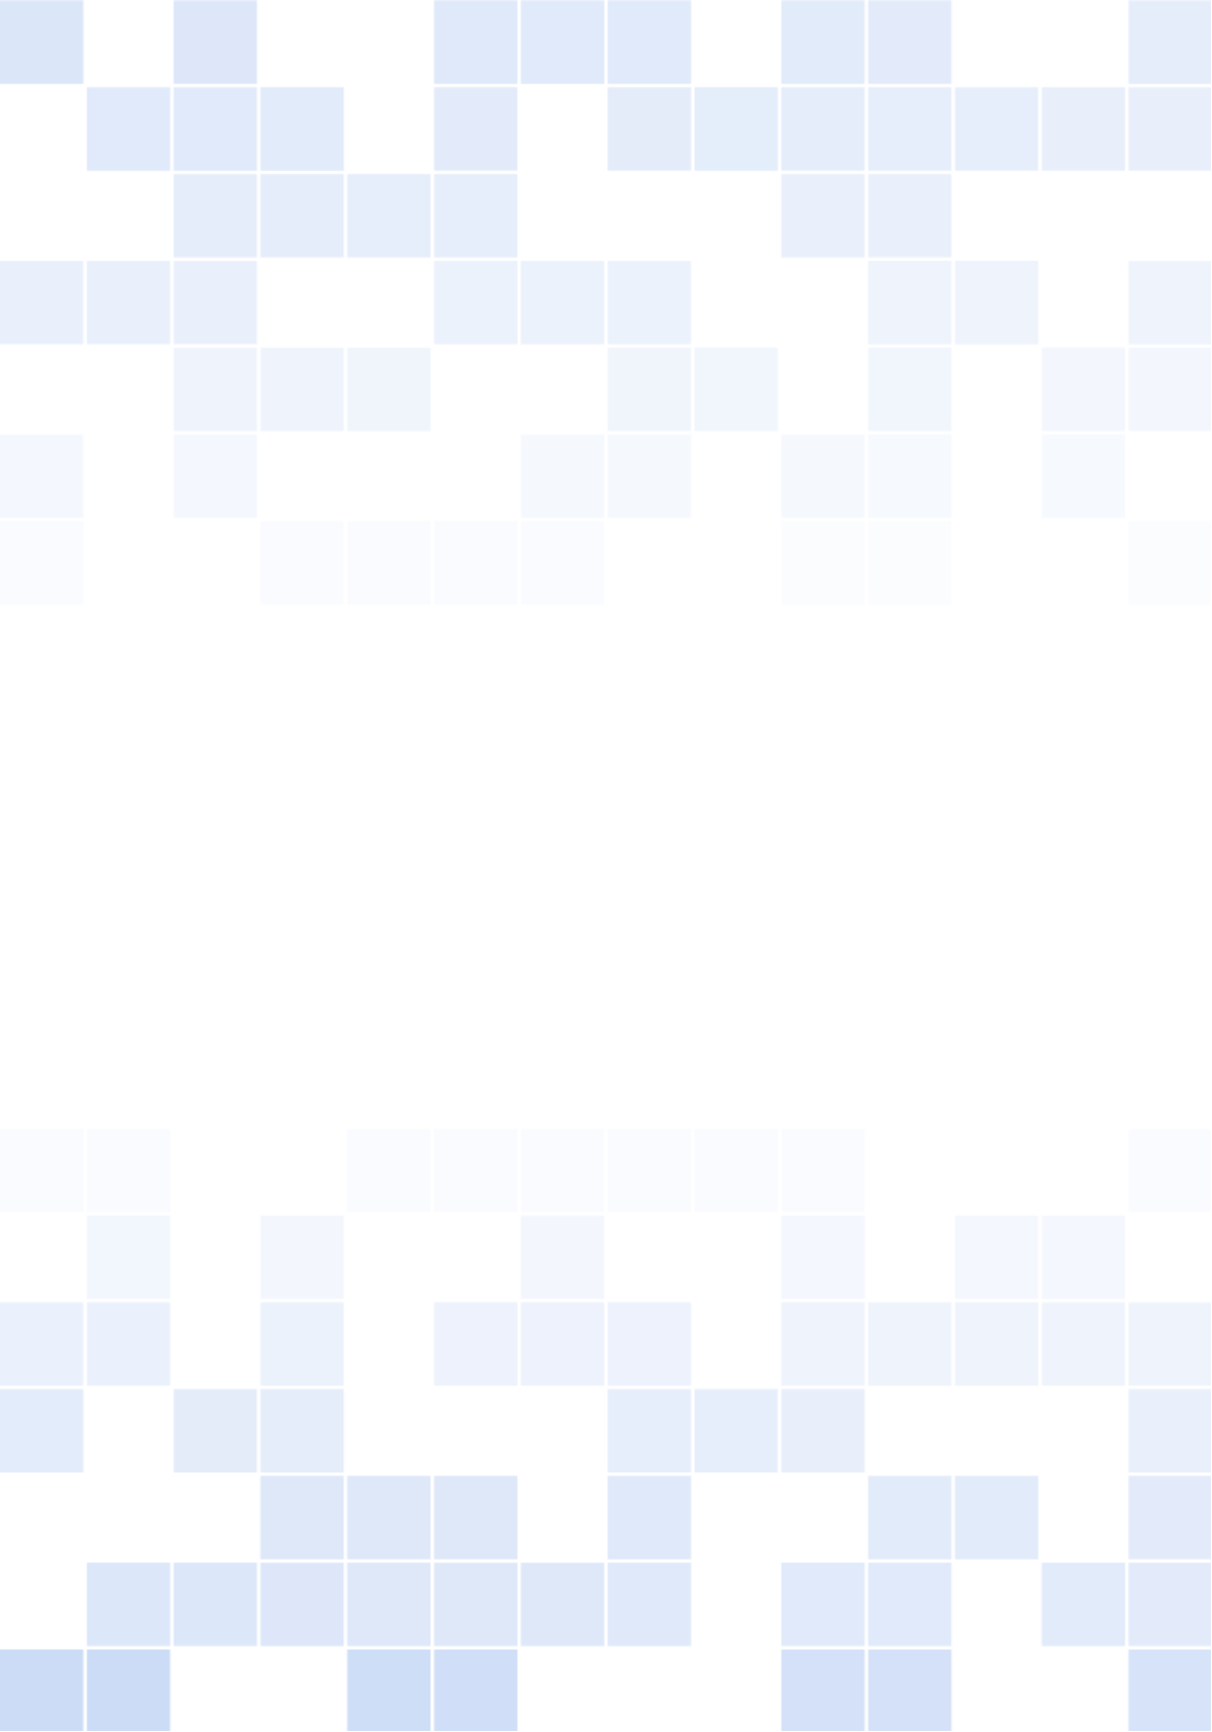
\includegraphics[width=\paperwidth]{background.pdf}};
\draw (current page.center) node [fill=ocre!30!white,fill opacity=0.6,text opacity=1,inner sep=1cm]{\Huge\centering\bfseries\sffamily\parbox[c][][t]{\paperwidth}{\centering El libro Azul de Inteligencia Artificial\\[15pt] % Book title
{\Large 1era Edición}\\[20pt] % Subtitle
{\huge Alejandro Medina Reyes}}}; % Author name
\end{tikzpicture}
\vfill
\endgroup

%----------------------------------------------------------------------------------------
%	COPYRIGHT PAGE
%----------------------------------------------------------------------------------------

\newpage
~\vfill
\thispagestyle{empty}

\noindent Copyright \copyright\ 2020 Alejandro Medina Reyes\\ % Copyright notice

\noindent \textsc{}\\ % Publisher

\noindent \textsc{}\\ % URL

\noindent Licensed under the Creative Commons Attribution-NonCommercial 3.0 Unported License (the ``License''). You may not use this file except in compliance with the License. You may obtain a copy of the License at \url{http://creativecommons.org/licenses/by-nc/3.0}. Unless required by applicable law or agreed to in writing, software distributed under the License is distributed on an \textsc{``as is'' basis, without warranties or conditions of any kind}, either express or implied. See the License for the specific language governing permissions and limitations under the License.\\ % License information, replace this with your own license (if any)

\noindent \textit{} % Printing/edition date

%----------------------------------------------------------------------------------------
%	TABLE OF CONTENTS
%----------------------------------------------------------------------------------------

%\usechapterimagefalse % If you don't want to include a chapter image, use this to toggle images off - it can be enabled later with \usechapterimagetrue

\chapterimage{chapter_head.pdf} % Table of contents heading image

\pagestyle{empty} % Disable headers and footers for the following pages

\tableofcontents % Print the table of contents itself


\pagestyle{fancy} % Enable headers and footers again

%----------------------------------------------------------------------------------------
%	PART
%----------------------------------------------------------------------------------------

\part{Parte uno}

%----------------------------------------------------------------------------------------
%	Prólogo y agradecimientos
%----------------------------------------------------------------------------------------

\chapterimage{chapter_head.pdf} % Chapter heading image

\chapter{Prólogo y agradecimientos}

\section{Prólogo}\index{Prólogo}

He decidido escribir este libro debido a que considero que es una rama de la computación muy interesante, además estos últimos años se ha incrementado el interés por la inteligencia artificial, debido principalmente a dos factores, la gran cantidad de información disponible que combinada con técnicas de deep learning nos permite hacer predicciones o generalizaciones muy exactas y el avance que hemos tenido tecnológicamente, siendo más preciso el desarrollo de potentes unidades de procesamiento gráfico, esto último es relevante ya que son capaces de trabajar eficazmente con operaciones de matrices que son ampliamente utilizadas por las redes neuronales.

A pesar de ser un campo con muchos años de investigación pienso que no hay mejor momento para descubrir todo el potencial que ésta área nos ofrece y explorar cómo puede repercutir en el mundo que nos rodea.

Este libro busca explorar diversos temas del campo de la inteligencia artificial con el fin de introducir diferentes paradigmas con los cuales se trabaja, revisando la parte conceptual y matemática, así como los usos de las diferentes técnicas.

%------------------------------------------------

\section{Agradecimientos}\index{Agradecimientos}

Primero quiero agradecer a mis padres ya que me han apoyado en todo mi desarrollo personal y académico, mis logros son un reflejo del gran ejemplo que me han dado y de lo mucho que han hecho por mi. Igualmente es importante reconocer el apoyo de mi hermana en las distintas actividades que he desempeñado y en los proyectos que me he propuesto.

También quiero agradecer a mis maestros que me han enseñado mucho a lo largo de mi carrera profesional, agradezco principalmente a aquellos que me han motivado a crecer y a perseguir mis sueños además de brindarme los conocimientos y herramientas del curso correspondiente. Entre mis maestros quiero darle las gracias especialmente a tres de ellos: José Jesús Sánchez Farías, José Guillermo Fierro Mendoza y Patricia Galvan Morales ya que sin su apoyo no creo que me hubiera decidido a hacer este libro.

Finalmente quiero darle gracias a mi amada esposa que me ha motivado a desarrollarme como persona y que siempre ha estado a mi lado dándome el impulso necesario para llevar a cabo este tipo de proyectos. 

%----------------------------------------------------------------------------------------
%	PART
%----------------------------------------------------------------------------------------

\part{Parte dos: Fundamentos}

%----------------------------------------------------------------------------------------
%	CHAPTER 3
%----------------------------------------------------------------------------------------

\chapterimage{chapter_head.pdf} % Chapter heading image

\chapter{Historia de la inteligencia artificial}

\section{Introducción}\index{Introducción - Historia de la IA}

Considero interesante revisar primero un poco de la historia de la Inteligencia Artificial, ya que nos permite ponernos en contexto acerca del estado actual de esta ciencia y cómo llegamos a este punto. También siendo una ciencia con muchas vertientes podemos analizar cuales fueron los aciertos y fallas del pasado para considerarlos en los desarrollos actuales.

\section{Ideas sobre inteligencia artificial}\index{Ideas sobre inteligencia artificial}

El deseo del ser humano por entender la inteligencia y ser capaces de replicarla se remonta a la antigüedad, un ejemplo es la existencia de Talos en la mitología griega, un gigante de bronce que protegía a la Creta minoica de posibles invasores, la versión más dominante de su origen dice que Talos era un autómata creado por Hefesto (Dios del fuego y la forja).

Existen otros ejemplos de autómatas antropomorfos como el robot de Leonardo da Vinci con la apariencia externa de una armadura, capaz de mover piernas y brazos o el autómata creado por Pierre Jacques-Droz en 1774, su creación podía escribir una carta compuesta por 50 caracteres determinados por el usuario.

%------------------------------------------------

\section{Orígenes de la inteligencia artificial}\index{Orígenes de la inteligencia artificial}

Si bien muchos consideran que el trabajo de Alan Turing “Computing Machinery and Intelligence” \cite{turing_compmach} dio inicio al campo de la inteligencia artificial creo relevante mencionar primero el trabajo realizado por Warren McCulloch and Walter Pitts en 1943, ese año publicaron "A logical calculus of the ideas immanent in nervous activity", aquí describieron un modelo de neurona que sentó las bases de lo que serían en un futuro las redes neuronales (Técnicas ampliamente usadas en la actualidad).

Posteriormente en 1950 Turing publico el trabajo mencionado anteriormente donde habló acerca del Test que lleva su nombre, mediante el cual en lugar de determinar si una máquina está “pensando”, tratamos de averiguar si es capaz de ganar en “el juego de la imitación” (Haciendo pensar a un ser humano que está hablando con otro humano), este trabajo fue de gran relevancia para el campo de la IA. Además del Test de Turing se cuestiono acerca de si una máquina puede realmente pensar y escribío algunas ideas sobre el desarrollo de máquinas capaces de aprender, este articulo es una lectura que yo personalmente considero de suma importancia para aquellos interesados en esta área.

\section{Nacimiento de la inteligencia artificial como ciencia}\index{Nacimiento de la inteligencia artificial como ciencia}

La conferencia de Dartmouth (“Dartmouth Summer Research Project on Artificial Intelligence”), realizada en 1956 y que duró 2 meses, es considerada como el evento que dio como resultado el nacimiento de la Inteligencia artificial como ciencia. 

En 1955 fue John McCarthy quien decidió organizar un grupo para estudiar la siguiente conjetura: cada aspecto del aprendizaje o característica de la inteligencia puede en principio ser descrito de manera tan precisa que una máquina pueda simularlo. A continuación muestro la propuesta de la conferencia \cite{DARTHMOUTH}: 

“We propose that a 2-month, 10-man study of artificial intelligence be carried out during the summer of 1956 at Dartmouth College in Hanover, New Hampshire. The study is to proceed on the basis of the conjecture that every aspect of learning or any other feature of intelligence can in principle be so precisely described that a machine can be made to simulate it. An attempt will be made to find how to make machines use language, form abstractions and concepts, solve kinds of problems now reserved for humans, and improve themselves. We think that a significant advance can be made in one or more of these problems if a carefully selected group of scientists work on it together for a summer.” 

Es aquí donde de forma oficial se introduce el término Inteligencia Artificial. (Si bien es un término que ya se había utilizado fue aquí donde se popularizó y se convirtió en el término dominante). Entre aquellos que asistieron se encuentran el Dr. Marvin Minsky, Herbert A. Simon, Allen Newell, Ray Solomonoff, John Henry Holland, entre otros. En este evento se discutieron diferentes acercamientos para crear soluciones de Inteligencia Artificial, los asistentes mencionados terminaron teniendo un alto impacto en esta ciencia.

\section{La edad de oro 1956-1974} \index{La edad de oro 1956-1974}

A la conferencia de Dartmouth le siguió un gran entusiasmo en el campo de la inteligencia artificial, incluso se estimaba que en 20 años se tendrían máquinas completamente inteligentes, a pesar de que era demasiado optimista si hubo avances durante este periodo de tiempo.

Entre los trabajos más relevantes se encuentran algoritmos que usan el paradigma “Reasoning as search”, en los cuales se aproximaba a la solución de problemas paso a paso como si de un laberinto se tratará, retrocediendo al llegar callejón sin salida, Allen Newell y Herbert A. Simon trataron de capturar una versión general de este algoritmo. También se dieron avances en el reconocimiento del lenguaje general, ELIZA desarrollado en el MIT permitía conversar mediante frases preprogramadas. A finales de 1960 Marvin Minsky y Seymour Papert propusieron que el estudio de la inteligencia artificial debía dirigirse a solucionar problemas en situaciones simples un enfoque denominado como micro-mundos, Minsky y Papert desarrollaron un robot que era capaz de apilar cubos. También se desarrolló el Perceptrón un tipo de red neuronal artificial que veremos más adelante en este libro.

\section{El primer invierno de la inteligencia artificial 1974-1980} \index{El primer invierno de la inteligencia artificial 1974-1980}

Debido a las altas expectativas desarrolladas previamente hubo una gran decepción al ver que las promesas de la Inteligencia Artificial no se cumplían. Hubo un gran recorte en los presupuestos de investigación y el campo de las redes neuronales fue mayormente ignorado debido a las fuertes críticas de Minsky sobre las limitaciones del perceptrón.

\section{El boom de la inteligencia artificial 1980–1987} \index{El boom de la inteligencia artificial 1980–1987}

La llegada de sistemas expertos (capaces de tomar decisiones como si fuese un experto humano mediante el uso de reglas lógicas) permitieron un nuevo boom en la Inteligencia Artificial gracias a su utilidad en las empresas.

Otro punto importante es el resurgimiento de las redes neuronales, gracias a las redes de Hopfield y el desarrollo del algoritmo de retropropagación.

\section{El segundo invierno de la inteligencia artificial 1987-1993} \index{El segundo invierno de la inteligencia artificial 1987-1993}

Durante este tiempo se dio otra reducción en las inversiones hacia el campo de la IA, sin embargo hubo avances principalmente en el campo de la robótica. Personalmente considero que una de las razones por las cuales tuvo lugar este segundo invierno de la IA son las desventajas o limitaciones de los sistemas expertos:

\begin{itemize}
\item Existen tareas demasiado complejas, la necesidad de diseñar estas reglas de manera manual es una limitante.
\item Existe conocimiento en constante cambio, muchos sistemas expertos requieren que las reglas sean actualizadas manualmente lo cual puede llegar a ser un problema.
\item Estos sistemas suelen contener conocimiento de un área específica pero carecen de sentido común. 
\end{itemize}

\section{Siglo XXI} \index{Siglo XXI}

Como mencione en el prólogo gracias a el aumento de potencia computacional y el acceso a grandes cantidades de información la Inteligencia Artificial ha visto grandes avances, entre los avances más notorios se encuentran las investigaciones y algoritmos de machine learning y deep learning.

\chapterimage{chapter_head.pdf} % Chapter heading image

\chapter{Fundamentos de la IA}

\section{Definición} \index{Definición}

Existen diferentes definiciones del término inteligencia artificial, de acuerdo a las ciencias de la computación la inteligencia artificial es el estudio de agentes inteligentes \cite{logical_approach}.

Un agente inteligente es capaz de percibir su entorno y actuar sobre él tratando de optimizar algún objetivo, un agente es inteligente debido a que presenta características como el razonamiento o el aprendizaje.

\begin{figure}[ht]
\centering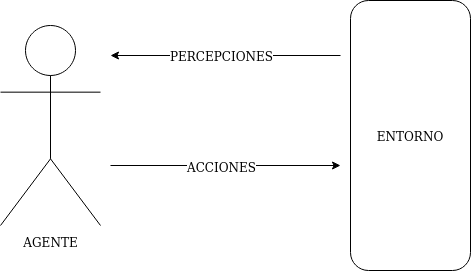
\includegraphics[width=7.5cm]{ia/Agente.png}
\caption{Representación de un agente}
\label{fig:agente} 
\end{figure}

Otra definición determina que la inteligencia artificial es el desarrollo de sistemas capaces de interpretar correctamente información externa, aprender de esta información para cumplir con ciertos objetivos o tareas adaptándose de manera flexible \cite{KAPLAN201915}.

Dependiendo de la definición diversos tipos de desarrollos pueden considerarse inteligentes o no, por ello yo prefiero una definición más abierta como la siguiente: la inteligencia artificial es la simulación de comportamientos inteligentes por parte de un sistema informático.

\section{Ciencias relacionadas con la IA} \index{Ciencias relacionadas con la IA}
La inteligencia artificial se relaciona con diversas ciencias que sirven de base para el desarrollo de esta ciencia, algunos ejemplos son los siguientes:

\begin{itemize}
\item Filosofía
\item Lógica/matemática
\item Ciencias computacionales
\item Psicología
\item Biología
\item Neurociencia
\end{itemize}

Es evidente como estas ciencias han ayudado al desarrollo de la inteligencia artificial, gracias a la teoría de la evolución se lograron generar algoritmos evolutivos, el estudio del cerebro nos dio ideas sobre la manera de tratar problemas como el reconocimiento de imágenes, la lógica nos permitió modelar la manera en la cual razonamos y gracias a la matemática somos capaces de formalizar los modelos para poder implementarlos en los sistemas desarrollados.

\section{Paradigmas de la inteligencia artificial} \index{Paradigmas de la inteligencia artificial}

De acuerdo a Palma y Marín \cite{marin2008inteligencia} existen 4 paradigmas principales:
\begin{enumerate}
\item Simbólico o representacional: El conocimiento se representa por medio de descripciones declarativas y en lenguaje natural, éstos son los hechos, otro conjunto de conocimientos son las reglas de inferencia que describen las relaciones sobre los hechos, al aplicar dichas reglas sobre un conjunto de conceptos de entrada se razona y se obtiene una inferencia.
Un ejemplo de este tipo de desarrollos son los sistemas expertos, este paradigma fue dominante desde 1956 a 1986.

\item Situado o reactivo: Toda conducta es resultado de una percepción, por lo cual éstas se tienen una conexión directa, condicionada o secuencial.

\item Conexionista: Describe que los problemas pueden ser resueltos por unidades pequeñas interconectadas entre sí. Las unidades pueden ser neuronas, genes, agentes inteligentes, etc. Este paradigma corresponde a las redes neuronales artificiales (RNA) se definen modelos con entradas y salidas en los cuales se ajustan parámetros de la red mediante diferentes algoritmos de aprendizaje. Dentro de este paradigma también entran los algoritmos evolutivos y sistemas multiagentes.

\item Híbrido: Para resolver diversos problemas existe la necesidad de integrar soluciones que corresponden a distintos paradigmas, por ello los sistemas híbridos son de gran utilidad para problemas reales.
\end{enumerate}

Una ventaja del paradigma simbólico es que es fácil interpretar lo que sucede dentro del sistema, en cambio en sistemas conexionistas suele ser complicado determinar las razones detrás de una decisión, sin embargo, actualmente se han desarrollado técnicas como Grad-CAM \cite{gradcam} que permiten reducir esta incertidumbre en el campo de clasificación de imágenes.

En la siguiente figura se muestran distintas categorías de técnicas de inteligencia artificial.

\begin{figure}[ht]
\centering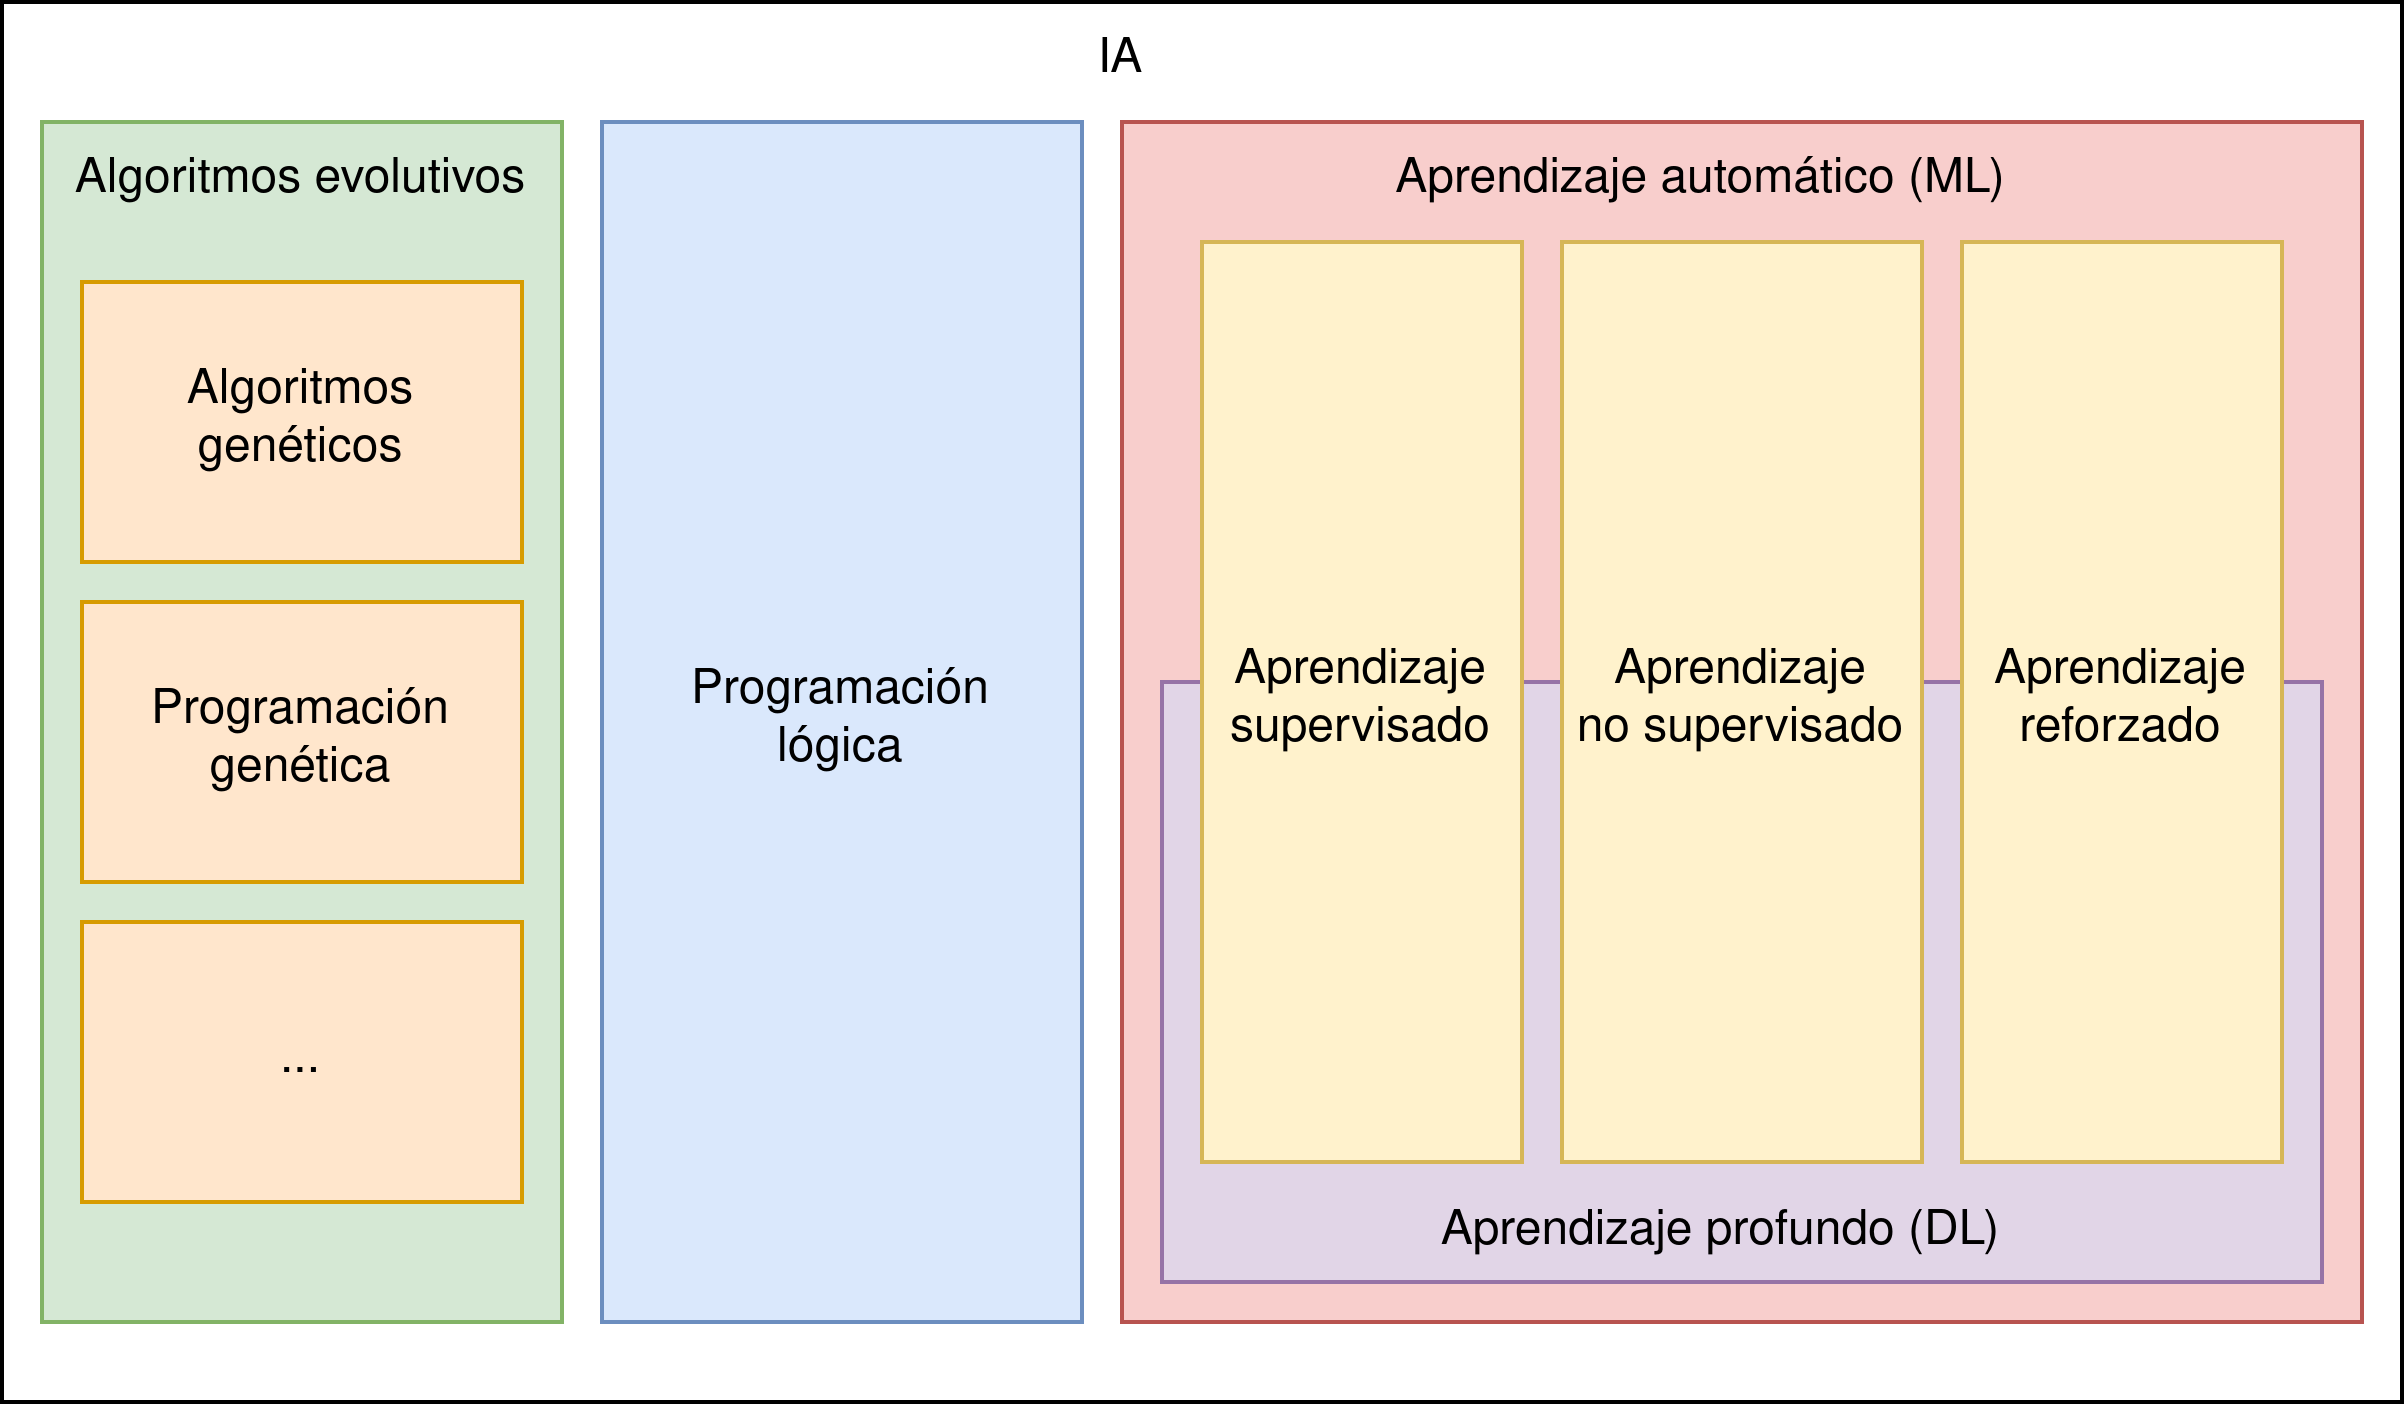
\includegraphics[width=13cm]{ia/ai_taxonomy.png}
\caption{Clasificación de técnicas de inteligencia artificial}
\label{fig:ai_taxonomy} 
\end{figure}

\part{Parte tres: Técnicas clásicas}

%----------------------------------------------------------------------------------------
%	CHAPTER 3
%----------------------------------------------------------------------------------------

\chapterimage{chapter_head.pdf} % Chapter heading image

\chapter{Búsquedas inteligentes}

\section{Introducción al capítulo}\index{Introducción al capítulo}

Antes de empezar a hablar directamente sobre estos temas relacionados principalmente con los grafos quiero hacer mención de un fenómeno descrito por John McCarthy “As soon as it works, no one calls it AI any more”; ésta frase me parece particularmente interesante debido a que la delimitación de los temas que comprenden la inteligencia artificial como ciencia no están perfectamente definidos, habrá autores que consideren estos temas como una rama de las estructuras de datos y no como parte de esta ciencia.

En los inicios de la inteligencia artificial era sorprendente cuando una máquina lograba algo remotamente inteligente y el asombro llevaba a generar altas expectativas del alcance de esta ciencia. Hoy en día quizá no se vea como algo tan sorprendente pero debido a que algunos de estos algoritmos nacieron siendo parte de la inteligencia artificial he decidido dedicarle una pequeña sección.

En este capítulo no profundizaré en las diversas técnicas de búsquedas inteligentes, en cambio revisaremos un ejemplo fuertemente ligado a la historia de la inteligencia artificial; sin embargo a continuación proporcionaré un link a el libro inteligencia artificial: introducción y tareas de búsqueda de Roberto J. de la Fuente López. (\url{http://www.aconute.es/iartificial/documentos/ia_intro_busqueda.pdf }) para aquellos que deseen abordar de una manera más amplia el tema.

\section{¿Qué es una búsqueda inteligente?} \index{¿Qué es una búsqueda inteligente?}

Una búsqueda inteligente es aquel algoritmo que nos permita recorrer una estructura de datos de manera eficiente para obtener una solución potencialmente óptima. 

\section{La IA que venció al campeón del mundo} \index{La IA que venció al campeón del mundo}

Son famosos los juegos entre Garry Kasparov y Deep blue, antes de ver el funcionamiento de esta computadora veremos un poco de la historia de estos encuentros.

Es poco mencionado el hecho de que Kasparov ganó la primera partida en 1996, se dieron seis juegos de los cuales 3 fueron ganados por Kasparov y uno por Deep Blue, los otros terminaron en empate. (Link de la victoria de Kasparov sobre Deep Blue: \url{http://hemeroteca.abc.es/nav/Navigate.exe/hemeroteca/madrid/abc/1996/02/19/084.html })

En la partida de 1997 Deep Blue derrotó a Kasparov, este último ganó un solo juego y Deep Blue ganó 2, los otros 3 quedaron en empate. Algo interesante es el hecho de que Kasparov acusó de hacer trampa a IBM \cite{hsu2004behind} después del segundo juego ya que mostraba signos de inteligencia o creatividad, IBM negó esto y dijo que solo se había dado intervención humana entre los juegos (lo cual estaba permitido en las reglas acordadas).

\section{¿Cómo funcionaba Deep Blue?} \index{¿Cómo funcionaba Deep Blue?}

El algoritmo detrás de Deep Blue no es tan inteligente como hace parecer, incluso uno de sus programadores (Joe Hoane) menciona en una entrevista que no es un proyecto de inteligencia artificial cuando se le preguntó cuánto de su trabajo era dedicado específicamente a la inteligencia artificial en emular el pensamiento humano \cite{DBFORBES}.

Las principales características de Deep Blue eran las siguientes 
\cite{CAMPBELL200257}:

\begin{itemize}
\item Libro de jugadas iniciales: Esto le permitía a la computadora realizar buenos movimientos iniciales
\item Hardware especializado: Deep Blue contaba con chips especializados que permitían evaluar tableros de ajedrez con una gran rapidez, la función de evaluación contaba con más de 8000 características y cada chip tenía una velocidad de búsqueda de 2 a 2.5 posiciones por segundo.
\item Paralelización de búsqueda: Deep Blue era un sistema con alta paralelización contando con más de 500 procesadores disponibles para realizar el árbol de búsqueda.
\end{itemize}
El algoritmo de búsqueda que utilizó Deep Blue está basado en el algoritmo alpha-beta que se detallará más adelante en este capítulo.

Si se quiere profundizar a detalle en el funcionamiento del sistema de esta computadora recomiendo leer el siguiente articulo (\url{https://doi.org/10.1016/S0004-3702(01)00129-1}). 

\section{El algoritmo Minimax} \index{El algoritmo Minimax}

El algoritmo de minimax nos permite elegir el mejor movimiento en un juego con adversario considerando que éste último siempre escogerá el peor movimiento para nosotros (el mejor para él).

En el juego existen dos jugadores:
\begin{enumerate}
\item Maximizador (MAX): trata de obtener la puntuación más alta.
\item Minimizador (MIN): trata de obtener la puntuación más baja.
\end{enumerate}
Algoritmo de minimax con movimientos alternativos:
\begin{enumerate}
\item Generación del árbol de juego. Se generarán todos los nodos hasta llegar a un estado terminal (o a alguna condición determinada).
\item Uso de función de evaluación sobre los nodos terminales.
\item Calcular el valor de los nodos superiores a partir del valor de los inferiores, dependiendo de si el nivel corresponde a MAX o MIN se escogerá el valor más alto o más bajo.
\item Elegir la jugada valorando los valores que han llegado al nivel superior.
Para ilustrar el funcionamiento de este algoritmo a continuación mostraré en imágenes los diferentes pasos con el ejemplo del juego de gato (Si X gana el estado vale 1, Si O pierde el estado vale -1, Si se empata el valor es 0):

\end{enumerate}

\begin{figure}[ht!]
\centering\includegraphics[width=9.5cm]{ia/generación_edos.png}
\caption{Generación de estados}
\label{fig:gen_edos_minimax} 
\end{figure}

\begin{figure}[ht!]
\centering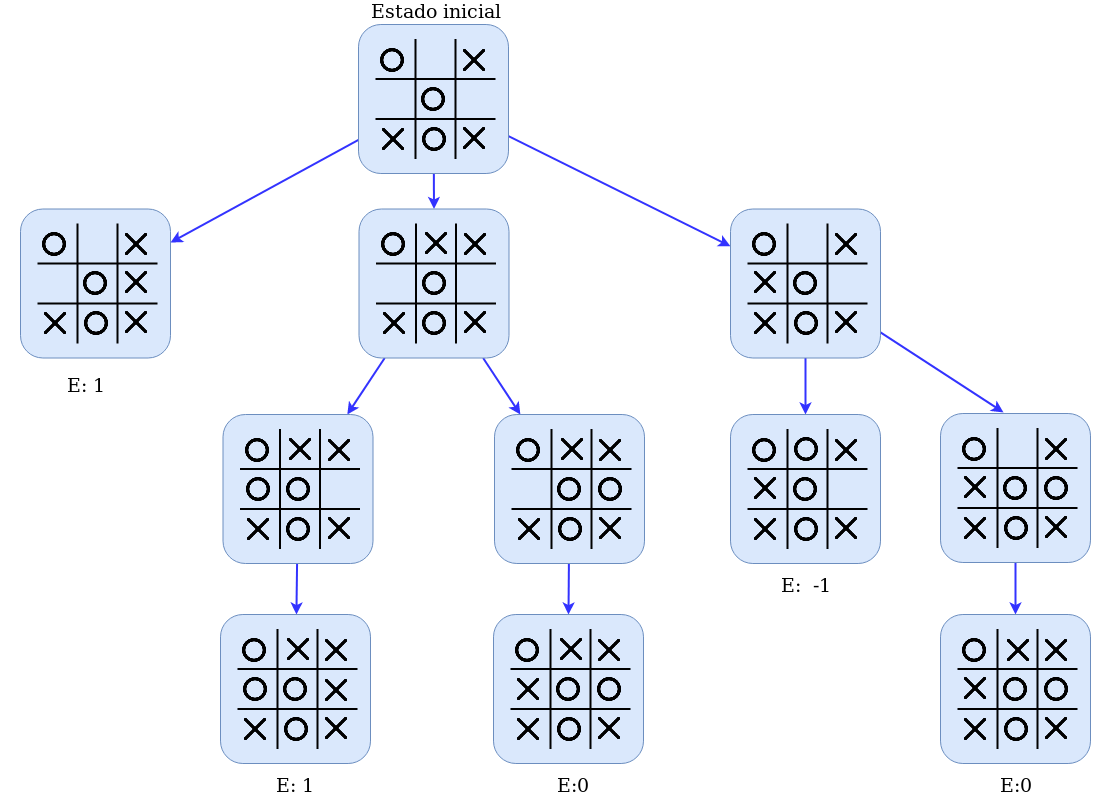
\includegraphics[width=11.5cm]{ia/evaluacion_edos_finales.png}
\caption{Evaluación de estados finales}
\label{fig:ev_edos_minimax} 
\end{figure}

\begin{figure}[ht!]
\centering\includegraphics[width=11.5cm]{ia/propagación_edos.png}
\caption{Cálculo de los valores en los nodos superiores}
\label{fig:prop_edos_minimax} 
\end{figure}

\begin{figure}[ht!]
\centering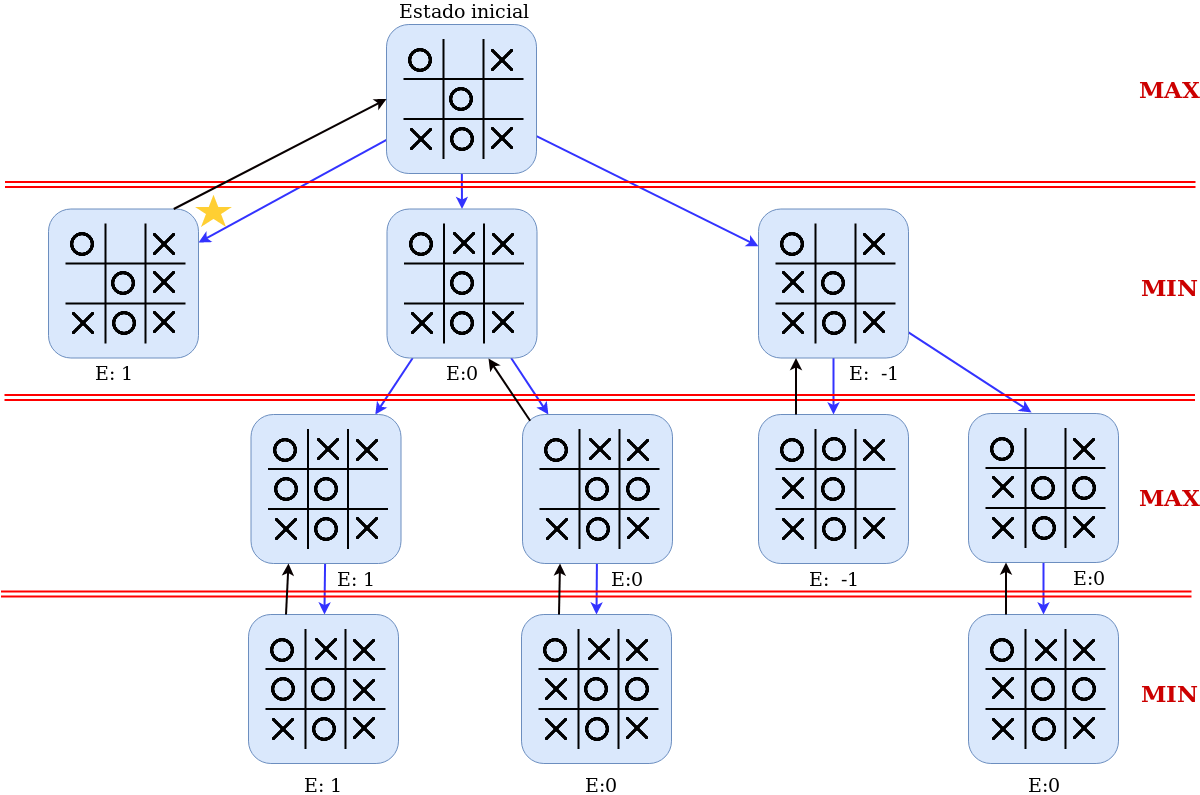
\includegraphics[width=13.5cm]{ia/eleccion_edo.png}
\caption{Elección de estado o jugada}
\label{fig:elec_edos_minimax} 
\end{figure}

\clearpage

El algoritmo MINIMAX es un procedimiento recursivo, a continuación se presenta el pseudocódigo correspondiente, se recomienda al lector analizar como el siguiente pseudocódigo hace lo mismo que se describió con anterioridad.


\begin{algorithm}
  \DontPrintSemicolon
  \SetKwFunction{FMain}{MINIMAX}
  
  \SetKwProg{Fn}{Función}{:}{}
  \Fn{\FMain{nodo, turnoMax}}{
  		\eIf{esTerminal(nodo)}{
  			funciónEvaluación(nodo)\;
  			\KwRet nodo\;
  		}{
  			posiblesEstados = funciónSucesor(nodo)\;
  			\ForEach{estado \textbf{in} posiblesEstados}{
  				estado = MINIMAX(estado, not (turnoMax) )\;
  				
  			}
  			\eIf{turnoMax}{
	  			\KwRet max(posiblesEstados)\;
	  		}{
	  			\KwRet min(posiblesEstados)\;
	  		}
  			
  		}
  }
  \;

  \caption{Algoritmo MINIMAX}
\end{algorithm}


Es importante notar que dependiendo del “juego” sobre el cuál se esté aplicando este algoritmo varía la función de evaluación y la función sucesor, encargada de generar los nuevos estados.

En el pseudocódigo descrito con anterioridad se generan todos los estados finales posibles, en el juego de gato esto no es un gran problema ya que el número de estados posibles es relativamente pequeño (alrededor de 362,800), sin embargo en otros juegos como el ajedrez este número es mucho más alto por lo cual se puede verificar a qué nivel de profundidad pertenece el nodo y si se ha llegado a ese límite establecido previamente evaluar el nodo aunque no sea un estado final, esto implica además el tener que generar funciones de evaluación más complejas ya que en ese punto no se puede saber con certeza si el jugador ganará o perderá.

Otra nota importante es que en este pseudocódigo es en los nodos donde se almacena el resultado de la evaluación, esto también podría hacerse implementando una tupla (nodo, valor) y devolviendo esta estructura en la función MINIMAX.

\begin{center}
\line(1,0){420}
\end{center}

\textbf{Ejercicio de programación:}

Yo recomiendo realizar el siguiente ejercicio para fortalecer los conocimientos adquiridos:
En cualquier lenguaje de programación programar una inteligencia artificial capaz de jugar gato utilizando el algoritmo Minimax. A continuación se presenta un enlace, se debe hacer una copia del notebook y seguir las instrucciones.

(Ejercicio para completar: \url{https://colab.research.google.com/drive/1xX4vcx6G0Dj_9XW5cml_lOnZnLIPb65T?usp=sharing})

(Ejemplo minimax web: \url{https://github.com/amr205/TicTacToe-AI---Minimax})



\includegraphics[width=5cm]{Pictures/github/minimax.png}

\clearpage

\section{El algoritmo Alpha-beta pruning} \index{El algoritmo Alpha-beta pruning}

El algoritmo Alpha-beta pruning tiene el objetivo de realizar la misma tarea que el algoritmo Minimax sin embargo poda las ramas que no necesitan ser revisadas, sigue regresando el mismo resultado que el algoritmo minimax pero reduce el nivel de nodos que visita.

En este caso incluiré primero el pseudocódigo y posteriormente procederé a explicar el funcionamiento de este algoritmo.

\begin{algorithm}
  \DontPrintSemicolon
  \SetKwFunction{FMain}{AlphaBeta}
  
  \SetKwProg{Fn}{Función}{:}{}
  \Fn{\FMain{nodo, turnoMax, alpha, beta}}{
  		\eIf{esTerminal(nodo)}{
  			funciónEvaluación(nodo)\;
  			\KwRet nodo\;
  		}{
  			posiblesEstados = funciónSucesor(nodo)\;
  			
  			\eIf{turnoMax}{
  				nodoMayor = nuevo Nodo\;
  				nodoMayor.valor = - infinito\;
  				
  				\ForEach{estado \textbf{in} posiblesEstados}{
	  				estado = AlphaBeta(estado, not(turnoMax), alpha, beta)\;
	  				alpha = max(alpha, estado.valor)\;
	  				nodoMayor = max(nodoMayor, estado)\;
	  				\If{beta <= alpha}{
	  					break
	  				}
	  			}
	  			
	  			\KwRet nodoMayor\;
	  		}{
	  			nodoMenor = nuevo Nodo\;
  				nodoMenor.valor = infinito\;
  				
  				\ForEach{estado \textbf{in} posiblesEstados}{
	  				estado = AlphaBeta(estado, not(turnoMax), alpha, beta)\;
	  				beta = min(beta, estado.valor)\;
	  				nodoMenor = min(nodoMenor, estado)\;
	  				\If{beta <= alpha}{
	  					break
	  				}
	  			}
	  			\KwRet nodoMenor\;
	  		}
  			
  		}
  }
  \;

  \caption{Algoritmo Alpha-Beta Pruning}
\end{algorithm}


Se puede observar que el funcionamiento es muy similar al algoritmo Minimax pero se utilizan dos variables, alpha y beta. Se puede observar que alpha guardaría el mejor estado posible que el maximizador tiene, y beta el mejor estado posible para el minimizador, por la manera en la que se visitan los nodos cuando beta es menor o igual no tiene mucho sentido continuar revisando la rama ya que el jugador contrario ya tiene una mejor opción en un nivel superior.

Un ejemplo de cómo funciona puede ser muy útil para entender el funcionamiento de este algoritmo, en lo personal considero que el siguiente video de Sebastian Lague muestra un ejemplo muy completo y descrito paso por paso (\url{https://youtu.be/l-hh51ncgDI?t=546}).

\begin{center}
\line(1,0){420}
\end{center}

\textbf{Ejercicio de programación:}

Yo recomiendo realizar el siguiente ejercicio para fortalecer los conocimientos adquiridos:

En cualquier lenguaje de programación programar una inteligencia artificial capaz de jugar ajedrez utilizando el algoritmo Alpha-beta pruning.


(Ejemplo: \url{https://github.com/amr205/Chess-AI-using-Alpha-Beta-pruning})



\includegraphics[width=5cm]{Pictures/github/alphabeta.png}

\chapterimage{chapter_head.pdf} % Chapter heading image

\chapter{Algoritmos evolutivos}

\section{Introducción al capítulo}\index{Introducción al capítulo}

Estos algoritmos inspirados en la evolución natural son útiles debido a que nos permiten tratar problemas que con técnicas de búsqueda no informada requerirían de un tiempo de proceso demasiado grande y con técnicas de búsqueda informada corren el riesgo de llegar a un óptimo local.

Una ventaja de los algoritmos evolutivos es que se requiere solo una pequeña cantidad de conocimiento específico sobre el problema que se está tratando, en concreto la función de evaluación (Fitness function) que debe ser optimizada en el proceso \cite{streichert2002introduction}, más adelante en este capítulo serán más evidentes las razones que llevan a esta afirmación.

\section{Orígenes} \index{Orígenes}

Desde la década de los 50s los científicos han estudiado este tipo de algoritmos, en 1954 Nils Barricelli creó el primer algoritmo genético que imitaba la reproducción y mutación natural, su objetivo no era resolver problemas de optimización, sino crear vida artificial. Durante los siguientes años científicos como Alexander Fraser usaron su trabajo, Fraser quería simular la evolución debido a que observarla de manera directa en nuestro mundo requeriría de millones de años.

John Holland es considerado una de las personas más importantes en el campo de los algoritmos genéticos, ya que él introdujo el uso de una población para evaluarla y posteriormente usar procesos como el crossover, recombination, etc. En 1975 publicó su libro que sería la base teórica de muchos trabajos posteriores.

En 1988 John Koza, patentó su idea de usar algoritmos evolutivos para la generación de programas, continuó su trabajo con múltiples publicaciones relacionadas con la programación genética, por lo cual su trabajo es de mucha importancia en esta área de los algoritmos evolutivos.

En 1986 Holland sentó las bases de los sistemas clasificadores (LCS), estos algoritmos tenían el objetivo de solucionar la tarea de clasificación y utilizan elementos de aprendizaje y algoritmos genéticos, Stewart Wilson continuó el desarrollo de nuevos sistemas clasificadores como el “Zeroth-level” usando métodos más modernos de aprendizaje reforzado.

\section{Definición} \index{Definición}

Los algoritmos evolutivos tienen su base en la selección natural, una definición que yo considero apropiada es la siguiente: Los algoritmos evolutivos mediante la heurística son capaces de resolver tareas de optimización imitando aspectos de la evolución natural, suelen trabajar en poblaciones completas de posibles soluciones para una determinada tarea (Streichert, 2002).

\textbf{NOTA: Diferencia entre un algoritmo evolutivo y un algoritmo genético}

Un algoritmo genético es una subclase de los algoritmos evolutivos.
Todo algoritmo evolutivo está basado en las leyes de la evolución natural, un algoritmo genético tiene sus bases en el uso de poblaciones, cruzamiento o recombinación (crossover) y mutación. En cambio otros tipos de algoritmos evolutivos se basan principalmente en la mutación.

\section{Clasificación} \index{Clasificación}

Existen distintos tipos de algoritmos evolutivos, en este capítulo se revisarán aquellos más populares, sin embargo también hay sistemas y algoritmos que presentan un comportamiento híbrido, estos algoritmos no serán cubiertos hasta que se hayan visto los temas necesarios para poder abordarlos de manera completa, un ejemplo de esto último es el algoritmo NEAT (NeuroEvolution of Augmenting Topologies) que combina los algoritmos genéticos con el paradigma conexionista.

A continuación se presentan los tipos de algoritmos evolutivos más comunes:

\begin{figure}[ht]
\centering\includegraphics[width=14cm]{ia/AE clasificación.png}
\caption{Clasificación de los algoritmos evolutivos más comunes}
\label{fig:classification-ae} 
\end{figure}

\section{Algoritmos genéticos} \index{Algoritmos genéticos} \label{section:Algoritmos-geneticos}

Los componentes principales de los algoritmos genéticos son los siguientes:
\begin{itemize}
\item Una función de evaluación a optimizar (fitness function)
\item Una población de cromosomas
\item Un operador de selección
\item Un operador de cruzamiento
\item Un operador de mutación
\end{itemize}

Antes de describir éstas partes, veamos el funcionamiento básico del algoritmo.
\begin{enumerate}
\item Se genera una población inicial
\item Se evalúa la población (si algún elemento supera algún nivel barrera se da por terminado el algoritmo)
\item Se seleccionan los mejores individuos de la población y se guardan en un grupo(en inglés a este grupo se le llama mating pool)
\item Se seleccionan pares del grupo generado y se aplica el operador de cruzamiento, también se aplica el operador de mutación de acuerdo a una tasa de mutación determinada por el desarrollador, al terminar la generación de la población se vuelve al paso 2.
\end{enumerate}

\begin{figure}[ht]
\centering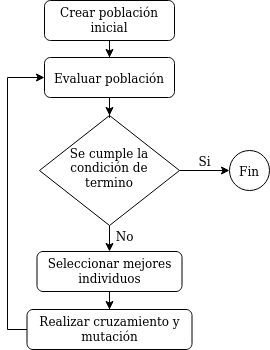
\includegraphics[width=5.5cm]{ia/GA.png}
\caption{Diagrama de flujo de un algoritmo genético}
\label{fig:df-ga} 
\end{figure}

A continuación se presenta un pseudocódigo de la implementación de un algoritmo genético simple, se recomienda leerlo y regresar a esta figura cuando se realice el ejercicio de programación propuesto.

\begin{figure}[ht]
\centering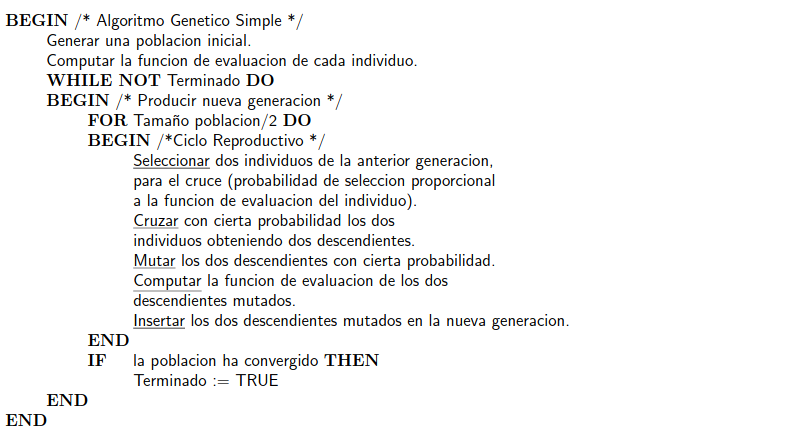
\includegraphics[width=13cm]{ia/pse-ga.png}
\caption{Pseudocódigo del Algoritmo Genético Simple, Figura tomada de Algoritmos Genéticos. 3 de Febrero 2020, de Universidad del País Vasco Sitio web: http://www.sc.ehu.es/ccwbayes/docencia/mmcc/docs/temageneticos.pdf}
\label{fig:pse-ga} 
\end{figure}

\subsection{Población}\index{Población}

Estos algoritmos trabajan sobre una población de cromosomas, el término cromosoma hace referencia a un valor o conjunto de valores que representan a una posible solución o individuo. A cada uno de estos valores dentro del cromosoma se les llama gen.

\begin{figure}[ht]
\centering\includegraphics[width=13cm]{ia/GA población, cromosoma, gen.png}
\caption{Población, cromosoma y gen}
\label{fig:pob-crom-gen} 
\end{figure}

chromosome = [p1,p2,...,pNpar]

\textbf{NOTA: Diferencia entre genotipo y fenotipo}

Al momento de hablar sobre la representación de los individuos de la población se suelen utilizar los términos genotipo y fenotipo, estos términos fueron creados por Wilhelm Johannsen en 1911, el genotipo es la información hereditaria completa de un organismo y el fenotipo son las propiedades observadas. En el campo de los algoritmos genéticos, el genotipo es una representación de bajo nivel (con menos abstracción) que el fenotipo.

\begin{figure}[ht]
\centering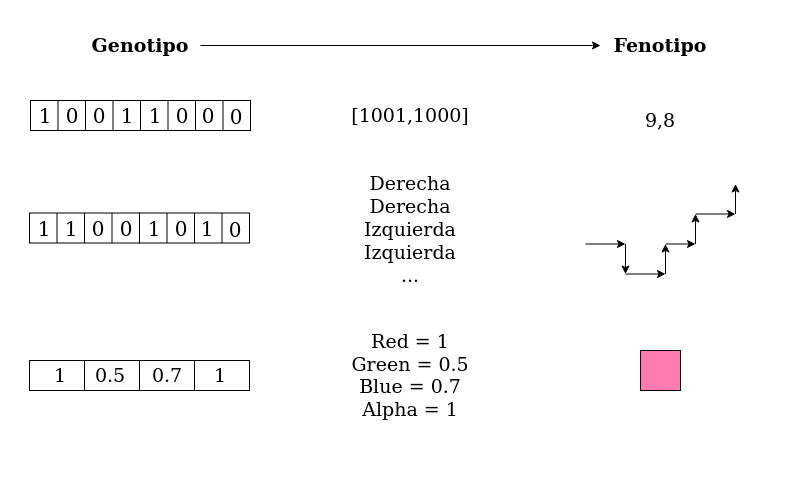
\includegraphics[width=13cm]{ia/ga - genotipo vs fenotipo.png}
\caption{Diferencia entre genotipo y fenotipo}
\label{fig:dif-gen-fen} 
\end{figure}

Es importante hacer notar que los genes no tienen que ser de tipo binario; un carácter o un elemento de alguna estructura (como un árbol) puede ser un gen por sí mismo.

Generalmente la población inicial es creada con valores al azar, un parámetro importante que el desarrollador debe determinar es el tamaño de la población ya que si el número es muy reducido no se tendrá suficiente variación y es posible que los individuos nunca sobrepasen un óptimo local, también se debe evitar poblaciones muy grandes para evitar la redundancia y para reducir el tiempo necesario para llegar a una solución adecuada.

\subsection{Evaluación}\index{Evaluación}

Para realizar la evaluación de los individuos se requiere tener conocimiento detallado sobre el problema que se está abordando, en algunas ocasiones se requiere realizar una simulación para encontrar el valor de aptitud (Fitness value), es común mantener el máximo valor en 1 y el menor en 0, para favorecer a los individuos con mejor aptitud se puede elevar a alguna potencia.

No siempre se trata de satisfacer un solo objetivo por lo cual a veces se tendrán distintas funciones enfocadas a evaluar los diferentes objetivos y estos deberán ser integrados en un solo valor.

Otra situación importante son los problemas con restricciones, para esto voy a proponer un ejemplo. Si quisiéramos diseñar un algoritmo genético capaz de resolver un sudoku, es probable que definiéramos el problema de la siguiente manera:

\begin{figure}[ht]
\centering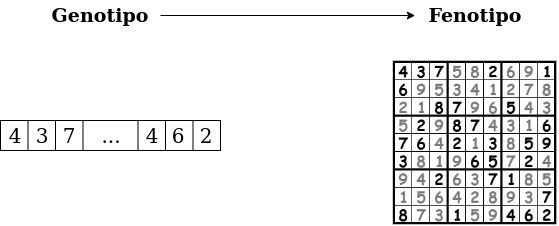
\includegraphics[width=11cm]{ia/sudoku ga - genotipo vs fenotipo.png}
\caption{Genotipo y fenotipo en un problema de resolución de sudoku}
\label{fig:sudoku-gen-fen} 
\end{figure}

Como se puede observar en la imagen anterior cada gen es un número del 1 al 9 que representa el valor que tendría en la casilla de la cuadrícula. Sin embargo se presentan ciertas restricciones:

\begin{enumerate}
\item No se pueden repetir números en un mismo renglón.
\item No se pueden repetir números en una misma columna.
\item No se pueden repetir números dentro de la misma subcuadrícula.
\item Se deben respetar los valores asignados a las casillas dados al momento 
	de plantear el problema.
\end{enumerate}

Para solucionar problemas con restricciones se pueden tomar diferentes medidas, las más comunes son reparación y penalización, la reparación evita que las restricciones sean violadas y la penalización disminuye el valor de aptitud de un individuo, más adelante se revisará la medida de reparación; en este subtema de evaluación se describe el proceso de penalización.

En este problema específico se podría tener una función como la siguiente:

$F(I) = \frac{(243-x-y-z)}{243}$

Siendo x el número de casillas repetidas en los renglones, y el número de casillas repetidas en las columnas y z el número de casillas repetidas en las subcuadrículas. En este problema la función depende altamente de las restricciones, pero supongamos que hacemos un algoritmo genético cuya función sea conducir en el menor tiempo posible con la restricción de no chocar ningún obstáculo, entonces podríamos definir una función que considerará el tiempo pero disminuyera la aptitud según el número de obstáculos golpeados.

$F(I) = \frac{(300-T-40*O)}{100}$

Siendo T el tiempo que se tardó el individuo en recorrer la pista y O el número de obstáculos golpeados.

\subsection{Selección}\index{Selección}\label{selection:pse-ga}

El proceso para la generación de una nueva población involucra el seleccionar padres para realizar el cruzamiento y la mutación, existen diversos métodos utilizados para realizar la selección de los padres, en este libro se explorarán las siguientes opciones \cite{SELECTION}:

\begin{enumerate}
\item Selección por ruleta (Roulette Wheel Selection)
\item Muestreo universal estocástico (Stochastic Universal Sampling)
\item Selección por rango lineal (Linear Rank Selection)
\item Selección por rango exponencial(Exponential Rank Selection)
\item Selección por torneo (Tournament Selection)
\item Selección por truncamiento (Truncation Selection)
\end{enumerate}


\underline{Selección por ruleta}

En este método la probabilidad de un individuo para ser elegido como padre es directamente proporcional a su valor de aptitud.

$p(i)=\frac{f(i)}{\sum_{j=1}^{n} f(j)}$
  
Donde n es el tamaño de la población y f(i) es la aptitud del individuo i

Una manera de implementar este método es el siguiente:
\begin{itemize}
\item Calcular el valor de $S$ ($S = \sum_{j=1}^{n} f(j)$)
\item Inicializar en 0 las variables: $p_{acumulada}$ y $j$
\item Generar un número al azar $\alpha$ entre los valores 0 y $S$
\item Mientras $p_{acumulada}<\alpha$  y   $j<n$:

\begin{itemize}
\item $p_{acumulada} = p_{acumulada} + f(j)$
\item $j = j+1$
\end{itemize}

\item Fin del ciclo
\item Seleccionar individuo j
\end{itemize}

Una desventaja de este método es el riesgo que existe donde el algoritmo genético termina de manera prematura en un óptimo local, esto debido a la presencia de un individuo con una aptitud considerablemente superior a la del resto de la población.

\underline{Muestreo universal estocástico}

Este método, desarrollado por Baker en 1987, es una variación del anterior y pretende eliminar el riesgo de convergencia prematura en un óptimo local.
Consiste en generar un número aleatorio $\alpha$ entre 0 y P (siendo P el promedio de la aptitud de los individuos) y posteriormente elegir a n individuos espaciados de manera uniforme (el valor de espaciado $\beta$ suele ser el promedio de la aptitud pero no es una regla).

\begin{figure}[ht]
\centering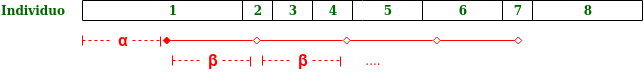
\includegraphics[width=13cm]{ia/GA SUS.png}
\caption{Elección de 5 individuos mediante muestreo universal estocástico}
\label{fig:ga-sel-mue} 
\end{figure}

\clearpage

Existen diferentes implementaciones de este algoritmo, yo recomiendo utilizar el siguiente proceso para seleccionar m individuos.
\begin{itemize}
\item Calcular el valor de $P$ ($P = \frac{1}{n} \sum_{i=1}^{n} f(i)$)
\item Inicializar en 0 las variables: $p_{acumulada}$, $j$ y $s$
\item Generar un número al azar $\alpha$ entre los valores 0 y $P$
\item Mientras $s<m$  y   $j<n$:

\begin{itemize}
\item $p_{acumulada} = p_{acumulada} + f(j)$
\item $j = j+1$
\item Si $p_{acumulada} < \alpha+s*\beta$

\begin{itemize}
\item Añadir elemento $j$ al conjunto $C$
\item $s = s+1$
\end{itemize}

\end{itemize}

\item Fin del ciclo
\item Devolver conjunto $C$
\end{itemize}

\underline{Selección por rango lineal}

Este método pretende evitar la convergencia del algoritmo genético en un óptimo local, es importante hacer notar que una desventaja es que disminuye la diferencia que hay entre los mejores y peores individuos por lo que puede aumentar el tiempo de convergencia, además de aumentar el tiempo de proceso necesario durante la generación de los rangos.

De manera intuitiva se puede decir que se le da un rango de 1 al peor individuo y al mejor un rango n, siendo n el tamaño de la población.

\begin{figure}[ht]
\centering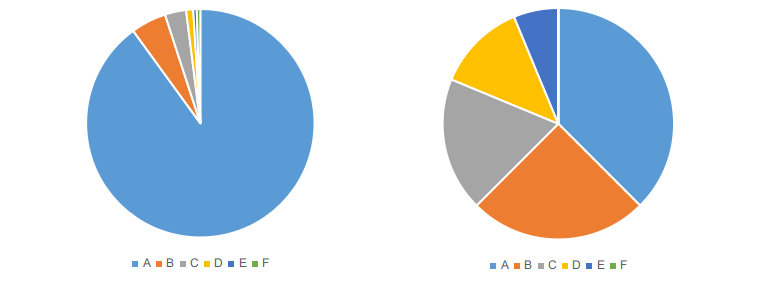
\includegraphics[width=14cm]{ia/seleclineal.png}
\caption{Ejemplo del cambio de probabilidad mediante el uso de selección por rango lineal (Derecha)}
\label{fig:ga-sel-lineal} 
\end{figure}

La fórmula que se usa para determinar la nueva aptitud en este método es de tipo lineal, un ejemplo sería el siguiente:

$f(pos) = \alpha + \frac{pos}{n}$

Mientras mayor sea el valor de $\alpha$ menor será la diferencia entre las probabilidades de los individuos, en la Figura \ref{fig:ga-sel-lineal} se usó 0 como valor de $\alpha$.

Otra fórmula que suele utilizarse es la siguiente:

$f(pos)=2-SP+\left ( 2*(SP-1)*\frac{pos-1}{n-1} \right )$

SP corresponde al término en inglés Selective Pressure (presión selectiva) y $2 \geq SP \geq 1$. A mayor presión selectiva más probabilidad de ser elegidos tienen los mejores individuos.

Para implementar este método se sugieren los siguientes pasos:
\begin{enumerate}
\item Ordenar los individuos de acuerdo a su aptitud
\item Calcular la nueva aptitud de acuerdo a una fórmula lineal
\item Implementar selección por ruleta
\end{enumerate}

\underline{Selección por rango exponencial}

Este método pretende aumentar la presión selectiva, se proponen diversas fórmulas, en este libro se sugiere la siguiente:

$f(pos)=exp(\frac{pos}{c})$

$c= \frac{n*2*(n-1)}{6*(n-1)+n} $

Existen distintos tipos de fórmulas que se pueden aplicar, es importante tratar de evitar fórmulas muy complejas que impacten altamente el tiempo de procesamiento, en la siguiente figura se observa una comparación que utiliza la fórmula propuesta aquí con anterioridad.

\begin{figure}[ht]
\centering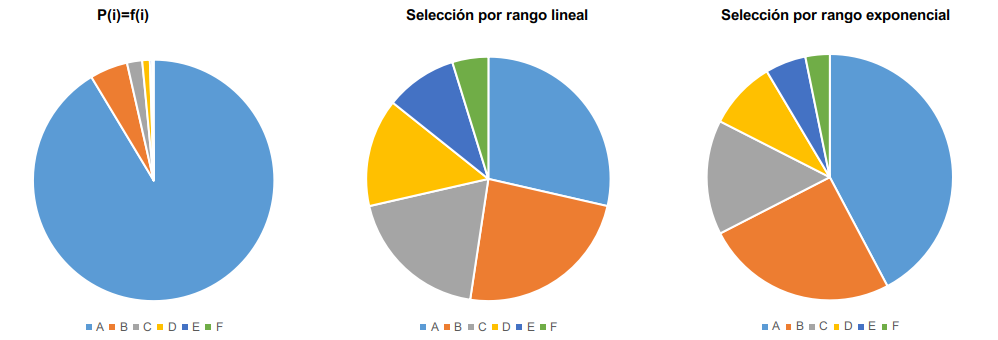
\includegraphics[width=14.5cm]{ia/sel-exp.png}
\caption{Comparación de probabilidad de selección entre tres métodos distintos}
\label{fig:comp_metodos} 
\end{figure}

Para implementar este método se sugieren los siguientes pasos:
\begin{enumerate}
\item Ordenar los individuos de acuerdo a su aptitud
\item Calcular la nueva aptitud de acuerdo a una fórmula exponencial
\item Implementar selección por ruleta
\end{enumerate}

\underline{Selección por torneo}

Este método consiste en obtener $k$ individuos y posteriormente seleccionar el individuo con mayor aptitud, este proceso se repite $n$ veces para obtener todos los padres.

La forma más fácil de implementar esta técnica es con $k=2$ se generan dos números aleatorios $\alpha$ y $\beta$ de 0 al tamaño de la población y se selecciona el elemento $\alpha$ o $\beta$  con mayor aptitud.

\underline{Selección por truncamiento}

Este método es bastante simple y no es muy utilizado en la práctica, su mayor caso de aplicación es en poblaciones de gran tamaño.

Consiste en ordenar los individuos de acuerdo a su aptitud y seleccionar una porción de los mismos para realizar la reproducción o cruzamiento entre ellos.

En el siguiente estudio Khalid Jeba \cite{SELECTION} analiza los métodos aquí descritos para estudiar el número de generaciones necesarias para llegar a la convergencia, así como el óptimo obtenido, también se propone un nuevo método que busca obtener un mejor óptimo sin sacrificar mucho tiempo para llegar a la convergencia. (\url{https://www.researchgate.net/publication/259009318_Parent_Selection_Operators_for_Genetic_Algorithms})


Otros métodos que me gustaría mencionar es la selección uniforme determinista que selecciona todos los elementos de la población para el cruzamiento, y la selección uniforme estocástica que selecciona elementos al azar de la población.

\subsection{Cruzamiento}\index{Cruzamiento}

Los operadores de cruce nos ayudan a generar la siguiente población a evaluar, consisten en generar 1 o más hijos a partir de dos individuos padre, el uso de algoritmos de cruzamiento lleva a un mejor desempeño en comparación a solo utilizar mutación, esto es más evidente cuando se tienen poblaciones grandes \cite{CROSSOVER_Spears}. Existen diversas maneras de realizar el cruzamiento, en este libro solo se revisarán algunos de los más comunes, más específicamente se revisarán los siguientes \cite{CROSSOVER_REVIEW}: Cruce de 1 punto, Cruce de k puntos, Cruce uniforme y Cruce por promedio.

\underline{Cruce de 1 punto}

Este es uno de los operadores de cruce más simples, dados dos individuos padres se elige un punto de cruce pi al azar, posteriormente se crean dos descendientes combinando los dos padres por el punto de cruce.

\begin{figure}[ht]
\centering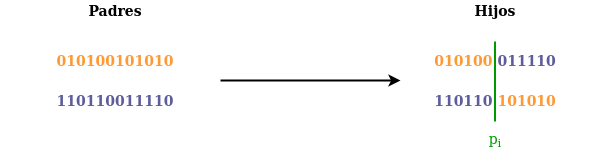
\includegraphics[width=15.5cm]{ia/GEC-1 punto.png}
\caption{Ejemplo de cruce de 1 punto, en este caso el punto de cruce se encuentra entre el sexto y el séptimo gen}
\label{fig:gec-1-punto} 
\end{figure}

\underline{Cruzamiento de k puntos}

Este operador es muy similar al anterior, la diferencia consiste en el número de puntos de cruce, se eligen k puntos de cruce para generar los descendientes.

\begin{figure}[ht]
\centering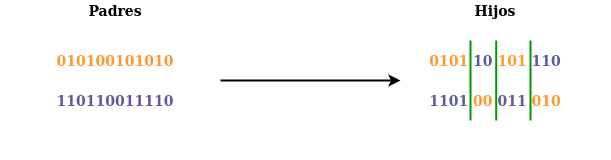
\includegraphics[width=15.5cm]{ia/GEC-k puntos.png}
\caption{Ejemplo de cruce de k-puntos, en este caso se usan 3 puntos de cruce}
\label{fig:gec-k-punto} 
\end{figure}

\underline{Cruce uniforme}

Este método consiste en combinar los genes de ambos padres, para cada gen se genera un número aleatorio que determina si el primer descendiente tomará el valor del gen del primer padre o del segundo. 

El pseudocódigo es similar al siguiente, dados dos padres a, b y dos descendientes x, y:

\begin{itemize}
\item Para cada gen
\begin{itemize}
\item Sea h un número aleatorio entre 0 y 1
\item Si h > 0.5
\begin{itemize}
\item El valor del gen para x es igual al valor del gen en a
\item El valor del gen para y es igual al valor del gen en b
\end{itemize}

\item Sino
\begin{itemize}
\item El valor del gen para x es igual al valor del gen en b
\item El valor del gen para y es igual al valor del gen en a
\end{itemize}
\end{itemize}
\end{itemize}

\underline{Cruce por promedio}

Este operador se utiliza cuando se tienen genes de tipo entero o real, dados dos padres se genera un solo descendiente, el valor de cada gen es el promedio del valor de los genes de los padres.

\begin{figure}[ht]
\centering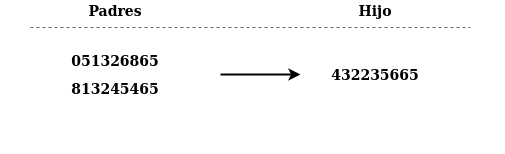
\includegraphics[width=14cm]{ia/GEC-promedio.png}
\caption{Ejemplo del uso del cruce por promedio}
\label{fig:GEC-promedio} 
\end{figure}

En el siguiente enlace pueden encontrar más técnicas de cruzamiento, algunas técnicas como el cruzamiento promediado se ajustan muy bien a cierto tipo de problemas por lo cuál puede valer la pena leer el siguiente artículo para observar si existe algún algoritmo de cruzamiento que se adapte a nuestro problema
(\url{http://ictactjournals.in/paper/IJSC_V6_I1_paper_4_pp_1083_1092.pdf}).

\subsection{Mutación} \index{Mutación}

La mutación permite que la población mantenga diversidad y mediante la generación de nuevos individuos no presentes en la población actual evita que el algoritmo converja en un valor prematuro.

Este operador se aplica sobre un cromosoma, dada una tasa de mutación (En inglés mutation rate) $p_{m}$ se genera un número aleatorio y si el número es menor a $p_{m}$ se realiza una o más modificaciones en los genes del individuo. En los algoritmos genéticos tradicionales (también llamados canónicos) el valor de $p_{m}$ es fijo, y solo se aplica un operador, sin embargo existen investigaciones que demuestran que es posible utilizar varios operadores con una tasa de mutación dinámica para cada operador, esto permite descubrir cuáles operadores son más útiles sin tener que realizar múltiples pruebas \cite{DYNAMIC_MUTATION}

\clearpage

\underline{Bit Flip Mutation}

Este operador se aplica para genes con valor binario, se selecciona uno o más genes y se invierte su valor.

\begin{figure}[ht]
\centering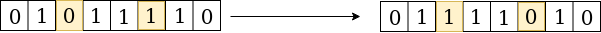
\includegraphics[width=15cm]{ia/Mutation-bitflip.png}
\caption{Aplicación del operador de mutación “Bit Flip”}
\label{fig:Mutation-bitflip} 
\end{figure}

\underline{Random Resetting}

Se selecciona uno o más genes y se le asigna al azar uno de los valores permitidos para el gen.

\begin{figure}[ht]
\centering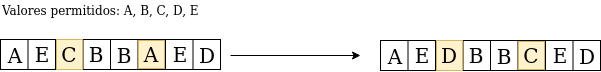
\includegraphics[width=15cm]{ia/Mutation-RANDOM RESET.png}
\caption{Aplicación del operador de mutación “Random Resetting”}
\label{fig:Mutation-RANDOMRESET} 
\end{figure}

\underline{Swap Mutation}

Consiste en seleccionar uno o más pares de genes e intercambiar su valor.

\begin{figure}[ht]
\centering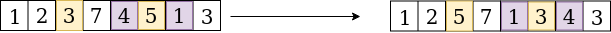
\includegraphics[width=15cm]{ia/Mutation-SWAP.png}
\caption{Aplicación del operador de mutación “Swap mutation”}
\label{fig:Mutation-SWAP} 
\end{figure}

\underline{Scramble Mutation}

Consiste en subconjunto de genes y ordenarlos de manera aleatoria para insertarlos nuevamente.

\begin{figure}[ht!]
\centering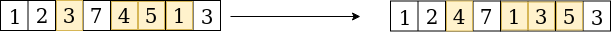
\includegraphics[width=15cm]{ia/Mutation-SCRABBLE.png}
\caption{Aplicación del operador de mutación “Scramble mutation”}
\label{fig:Mutation-SCRABBLE} 
\end{figure}

\underline{Inverse Mutation}

Consiste en subconjunto de genes e invertir su orden para insertarlos nuevamente.
\begin{figure}[ht!]
\centering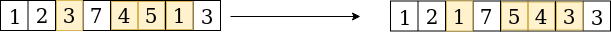
\includegraphics[width=15cm]{ia/Mutation-Inverse.png}
\caption{Aplicación del operador de mutación “Inverse mutation”}
\label{fig:Mutation-Inverse} 
\end{figure}

\subsection{Resolver problemas con restricciones} \index{Resolver problemas con restricciones}

Anteriormente en la sección correspondiente a la evaluación en los algoritmos genéticos se exploró el problema del sudoku como una situación donde existen restricciones, las tres maneras más comunes de implementar algoritmos con este tipo de problemas son las siguientes:

\begin{enumerate}
\item Uso de Funciones de penalización que reducen severamente el valor de aptitud de los individuos que no satisfacen las restricciones.
\item Uso de Funciones de reparación que toman una solución y la modifican para que cumpla con todas las restricciones.
\item No permitir que se genere ningún individuo que no cumpla con las restricciones.
\end{enumerate}

\subsection{Elitismo en algoritmos genéticos} \index{Elitismo en algoritmos genéticos}

El elitismo en los algoritmos genéticos consiste en asegurar que un porcentaje de los mejores individuos pasen a la siguiente generación de la población, se recomienda mantener este porcentaje por debajo del 10\% para asegurar la diversidad de la población. Usualmente estos individuos pasan a la siguiente generación sin ninguna mutación, posteriormente se realiza el proceso de crossover y mutación de manera habitual para completar la nueva población.

\textbf{¿Porqué utilizar elitismo?}

Usar elitismo puede tener un alto impacto en el rendimiento de nuestro algoritmo (Aumentando la velocidad de convergencia) \cite{rani2019effectiveness} debido a que no se tienen que re-descubrir soluciones que ya han probado tener una alta aptitud. De esta manera se asegura también que la aptitud del mejor individuo nunca va a reducirse a través del paso de las generaciones de la población.

\textbf{¿Porqué NO utilizar elitismo?}

Usar elitismo puede hacer al algoritmo converger en un óptimo local de manera prematura, esto depende también del porcentaje de la población que se use para aplicar el elitismo, mientras mayor sea el porcentaje mayor riesgo se corre de limitar el espacio de búsqueda de nuestro algoritmo.

\textbf{Implementación}

La manera más simple de implementar elitismo es ordenando los elementos de la población de acuerdo a su aptitud para posteriormente copiar el porcentaje de cromosomas determinados con anterioridad por el desarrollador, es importante no sobrescribir los valores de estos elementos por lo que solo se deben generar la cantidad de individuos restantes de la población.

\subsection{Aplicaciones de los algoritmos genéticos} \index{Aplicaciones de los algoritmos genéticos}

Los algoritmos genéticos resultan extremadamente para resolver problemas de parametrización, en problemas con múltiples óptimos locales las soluciones basadas en gradientes no suelen resolver el problema por lo cual los algoritmos genéticos son una buena alternativa.
\begin{itemize}
\item Machine learning: Se pueden utilizar los algoritmos genéticos para crear sistemas que aprendan reglas de producción o sistemas clasificadores (Wang, Bayer)
\item Multimodal optimization: Los algoritmos genéticos nos pueden ayudar a encontrar múltiples soluciones en contraste a solo una.
\item Problemas de ingeniería: Si se posee el conocimiento suficiente para crear una buena función de evaluación se pueden resolver problemas de diversas áreas de la ingeniería.
\end{itemize}

\subsection{Construcción de un algoritmo genético} \index{Construcción de un algoritmo genético}

A continuación se presenta una tabla que resume los puntos que el desarrollador debe determinar o tomar en cuenta cuando construye un algoritmo genético.

\begin{table}[ht!]
\centering
\caption{Parámetros y consideraciones en la construcción de un algoritmo genético}

\begin{tabular}{|p{5cm}|p{9cm}|}
\hline
	Parámetros de la población & Tamaño de la población\\
\hline
	Representación de la población & Método de selección y parámetros del método seleccionado. Ej. Si se selecciona Selección por rango lineal se debe determinar el valor de Selective Pressure \\
\hline
	Cruzamiento & Método de cruzamiento\\
\hline
	Mutación & Implementación de la mutación sobre nuestra población y  tasa de mutación\\
\hline
	Elitismo & Determinar si se usará o no y el porcentaje de la población que pasaría a la siguiente generación mediante elitismo.\\
\hline
	Terminación & Determinar la condición de finalización\\
\hline

\end{tabular}
\end{table}

\FloatBarrier

\begin{center}
\line(1,0){420}
\end{center}

\textbf{Ejercicio de programación:}

Ejercicio para fortalecer los conocimientos adquiridos:

En cualquier lenguaje de programación hacer un programa capaz de realizar alguna de las siguientes tareas:

\begin{itemize}
\item Resolver un tablero de sudoku con algunas celdas llenadas previamente.
\item Resolver el problema del viajero. 
	(\url{https://es.wikipedia.org/wiki/Problema_del_viajante})
\item Adaptar la posición y rotación de líneas en un espacio tridimensional para 	representar una imagen. (\url{https://youtu.be/iV-hah6xs2A})
\end{itemize}
A continuación se presenta un repositorio donde aplicó un algoritmo genético para solucionar tableros de sudoku:


\includegraphics[width=5cm]{Pictures/github/genetic.png}

\url{https://github.com/amr205/SudokuSolver---Genethic-Algorithm}

\section{Programación genética} \index{Programación genética}

En este libro se revisarán las bases de la programación genética para culminar con un proyecto que demuestre que se entienden estos conceptos y se poseen las habilidades de programación necesarias para poner en práctica lo aprendido. Si tú como lector quieres explorar más a profundidad este tema recomiendo leer el siguiente libro:



(\url{http://www.lulu.com/shop/riccardo-poli-and-william-b-langdon-and-nicholas-freitag-mcphee/a-field-guide-to-genetic-programming/ebook/product-17447670.html}).

\clearpage

\textbf{¿Qué es la programación genética?}

La programación genética es un tipo de algoritmo evolutivo en el cual se determina “que debe hacerse” y se generan programas computacionales para resolver dicho problema.

El funcionamiento general de la programación genética es muy similar a los algoritmos genéticos ya que también tiene su base en la selección natural de la teoría de la evolución de Darwin. De hecho son tan similares que la Figura \ref{fig:df-ga} presentada para los algoritmos genéticos describe igualmente el flujo de un programa que implementa programación genética.

\textbf{Diferencia entre un algoritmos genéticos y la programación genética}

La respuesta más simple a esta pregunta son los individuos de la población, en la programación genética cada individuo es un programa computacional.
Como se verá a continuación esto impacta en la representación de nuestros individuos, generación de la población y en los métodos de cruzamiento y mutación.

\subsection{Tipos de programación genética}\index{Tipos de programación genética}

De acuerdo a la representación de los programas existen diferentes tipos de programación genética, en este libro se abordará el tipo basado en árboles debido a que es uno de los tipos más comunes.

\textbf{Programación genética basada en árboles}

En este tipo de PG el programa se representa mediante árboles, este tipo de representaciones son bastante comunes y suelen usarse para resolver problemas de un dominio específico. Este tipo de representación suele trabajar muy bien con lenguajes funcionales, una de las primeras implementaciones fue en el lenguaje LISP debido a que la estructura del lenguaje se presta para utilizar este tipo de algoritmos.

John Koza \cite{koza1992genetic} menciona que esta representación es más natural que una basada en cadenas de caracteres de longitud fijo (o representaciones de tipo cromosoma) debido a que permite a los programas de la población tener variedad en su tamaño y longitud.

\begin{figure}[ht]
\centering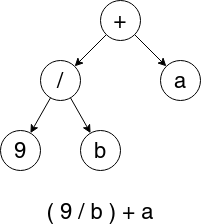
\includegraphics[width=5cm]{ia/GP-tree.png}
\caption{Representación de un programa mediante un árbol.}
\label{fig:GP-tree} 
\end{figure}

\textbf{Programación genética lineal}

Este tipo de representación se asemeja mucho más a los lenguajes imperativos ya que los programas son representados como una serie de instrucciones.

Es importante notar la diferencia entre este tipo de algoritmos y los algoritmos genéticos, una de las diferencias claves consiste en el hecho de que los programas generados pueden tener diferente tamaño (cantidad de instrucciones). A pesar de su estructura lineal este tipo de programación genética es capaz de generar soluciones para problemas de alta complejidad \cite{opensourceLGP}. En la siguiente figura se puede observar una comparación entre la representación lineal y la representación lineal.

\begin{figure}[ht]
\centering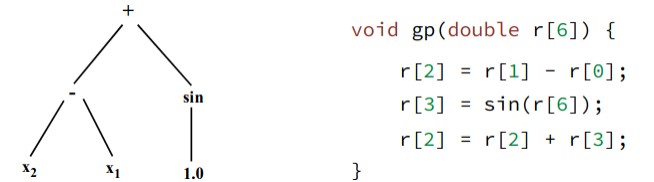
\includegraphics[width=14cm]{ia/gp-tree1e1.png}
\caption{Comparación entre la representación basada en árboles (izquierda) y la representación lineal, el array proporcionado como argumento para el algoritmo de programación genética lineal es el siguiente r={x1,x2,1.0,1.0,0.0,1.0}, Figura tomada de Jed Simson. (2017). Open-Source Linear Genetic Programming. : Faculty of Computing and Mathematical Sciences University of Waikato, Waikato, New Zealand.\cite{opensourceLGP}}
\label{fig:gp-tree1e1} 
\end{figure}

\textbf{Otros tipos de programación genética}

Existen otros tipos de representaciones como la evolución gramatical que utiliza la estructura gramatical del lenguaje para generar programas, así como otros tipos de representaciones, sin embargo estos tipos de PG se encuentran fuera del alcance de este libro.

\subsection{Representación de los individuos}\index{Representación de los individuos}

NOTA: Como se mencionó anteriormente este libro está centrado en la programación genética basada en árboles, por lo cual todos los subtemas posteriores del tema de programación genética usan solamente esta representación.

Los programas que se generan no suelen ser programas completos como los que nosotros como desarrolladores desarrollamos, en cambio suelen ser de dominios más específicos. Como se mencionó anteriormente los programas suelen representarse como árboles sintácticos, en formas más avanzadas de la programación genética, el programa consta de diferentes subrutinas unidas entre sí, en este libro solo se tratará la forma básica que consiste de un solo árbol sintáctico \cite{opensourceLGP}.

Para formar el árbol sintáctico se utilizan un conjunto de funciones y un conjunto de elementos terminales, los nodos internos utilizan elementos del conjunto de funciones y las hojas del árbol toman valores del conjunto de elementos terminales. Estos conjuntos deben contener los elementos suficientes para poder generar soluciones apropiadas para nuestro problema planteado.

\begin{figure}[ht]
\centering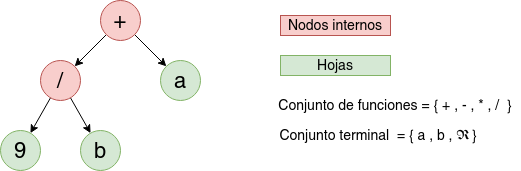
\includegraphics[width=14cm]{ia/GP-tree2.png}
\caption{Árbol sintáctico de la operación (9 / b)+a.}
\label{fig:GP-tree2} 
\end{figure}

\textbf{Conjunto terminal}

Este conjunto puede contener los siguientes elementos \cite{opensourceLGP}:
\begin{itemize}
\item Constantes: Estas suelen ser generadas de manera aleatoria durante la creación del árbol o creadas durante el proceso de mutación. El símbolo $\Re$ representa una constante aleatoria efímera (En inglés llamada ephemeral random constant), esta constante representa un conjunto de constantes fijas. Ej $\Re = \{ x | x$ es un entero y $0 \leq x \leq 10 \}$
\item Funciones sin argumentos: Este tipo de funciones pueden regresar un valor distinto cada vez que se usan, un ejemplo sería una función que genere un número aleatorio.
\item Valores de entrada externos: Son los argumentos del algoritmo de PG, suelen ser representados con el nombre de alguna variable, en la Figura \ref{fig:GP-tree2} a y b serían un ejemplo de este tipo de elementos.
\end{itemize}

\textbf{Conjunto de funciones}

Las funciones estarán determinadas por el tipo de problema que se necesita resolver, en el caso de la Figura \ref{fig:GP-tree2} las funciones son de carácter aritmético.
Para que nuestro algoritmo de PG funcione de manera correcta se tienen que cumplir dos propiedades: consistencia de tipo y seguridad en la evaluación.

\underline{Consistencia de tipos}

Para cumplir con la consistencia de tipo todas nuestras funciones tienen que utilizar argumentos del mismo tipo y devolver valores del mismo tipo, esto puede limitar el tipo de funciones que podemos incluir en nuestro conjunto, sin embargo algunas funciones pueden ser re-interpretadas para que trabajen con el mismo tipo que las demás. Ejemplo: Las función IF-THEN trabaja con dos argumentos, uno booleano y uno numérico, si la quisiéramos usar con operadores aritméticos podríamos reestructurarla para que tome tres argumentos numéricos y si el primer argumento sea mayor al segundo devuelva el valor del tercero, así se habría conservado la consistencia de tipos.

Si no se cumple la consistencia de tipos se tendrían que implementar medidas en la fase de cruzamiento y mutación que asegurarán que los árboles generados siguieran siendo válidos.

\underline{Seguridad en la evaluación}

Básicamente se debe evitar que el programa produzca errores al ejecutarse, un ejemplo claro es el de la división sobre cero. Se pueden tomar distintas acciones para tratar este tipo de situaciones, la primera es reducir altamente la aptitud de los programas que produzcan errores, la segunda es utilizar funciones adaptadas para responder con algún valor ante estas situaciones, la función de división protegida, denotada comúnmente con el símbolo \% suele devolver un valor de 1 ante una división sobre 0.

\subsection{Generación de la población inicial} \index{Generación de la población inicial}

Existen diferentes maneras en las cuales se puede generar la población inicial, tener programas duplicados en nuestra población es un gasto de recursos computacionales por lo que se sugiere evitar que se generen, sin embargo es recomendable pero no necesario \cite{koza1992genetic}. A continuación se describen dos técnicas básicas (y comunes) para generar una población inicial.

\clearpage
\underline{Full}

El desarrollador define una profundidad de los programas, se genera un nodo raíz a partir del conjunto de funciones y se va formando el árbol a partir de estos elementos hasta que se llega a la profundidad definida, en ese momento se seleccionan elementos del conjunto terminal.

\begin{figure}[ht]
\centering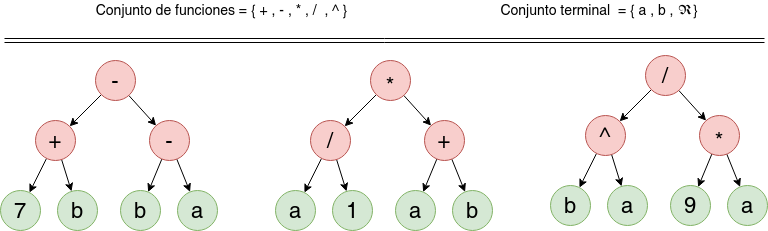
\includegraphics[width=14cm]{ia/Full -GP.png}
\caption{Ejemplo de tres individuos de un población generada con el método full con una profundidad de 3.}
\label{fig:Full-GP} 
\end{figure}

\underline{Grow}

El desarrollador define la profundidad máxima de los programas, cuando se generan los nodos del árbol estos se generan a partir de la combinación del conjunto de funciones y el conjunto terminal, si se llega a la profundidad máxima solo se seleccionan elementos del conjunto terminal. Esto permite generar árboles con distinto tamaño.

\begin{figure}[ht]
\centering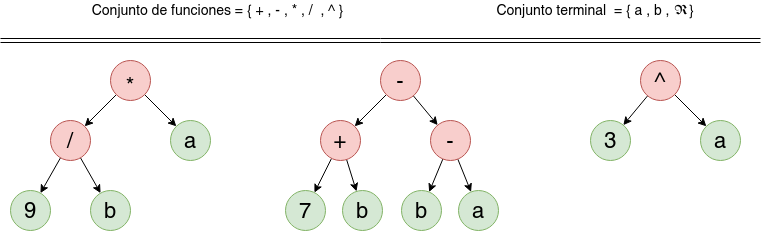
\includegraphics[width=14cm]{ia/GROW-GP.png}
\caption{Ejemplo de tres individuos de un población generada con el método grow con una profundidad de 3.}
\label{fig:GROW-GP} 
\end{figure}

Koza \cite{koza1992genetic} sugiere generar la mitad de la población usando el método full y la otra mitad usando el método grow, al uso de esta combinación se le conoce como “ramped half and half”.

\subsection{Evaluación de los individuos} \index{Evaluación de los individuos}

La evaluación de la aptitud de los individuos depende ampliamente del tipo de problema que se trata de resolver, para evaluar un individuo se tiene que ejecutar el programa, en problemas donde tenemos un conjunto de entradas con su correspondiente salida, se podría calcular el resultado con base en la diferencia entre el resultado proporcionado por el programa y el resultado esperado.

$\frac{1}{m} \sum_{i=0}^{m}(y_i-x_i)^{2}$

Donde $m$ es el tamaño del conjunto que contiene las entradas con la salida correspondiente, $y_i$ es la salida esperada y $x_i$ es la salida obtenida.

Como se mencionó anteriormente se deben penalizar los programas que generen errores en su ejecución.
Muchos de las aplicaciones prácticas requieren de funciones de evaluación multiobjetivo, en este caso se podría analizar la diferencia entre el resultado esperado y el obtenido, el tiempo de ejecución, y los recursos de memoria utilizados, de esta manera se podría obtener una solución que encontrará un buen balance entre estos tres aspectos.

Para correr el programa se puede construir la sentencia para ejecutar en algún lenguaje como por ejemplo LISP, otra opción es evaluar nuestro programa dentro del mismo lenguaje haciendo uso de una función de evaluación, a continuación se presenta un algoritmo que realiza esta última tarea, se recomienda al lector interiorizar y reflexionar sobre el algoritmo que se presenta a continuación y como usa la recursividad para obtener el valor del programa.

\begin{figure}[ht]
\centering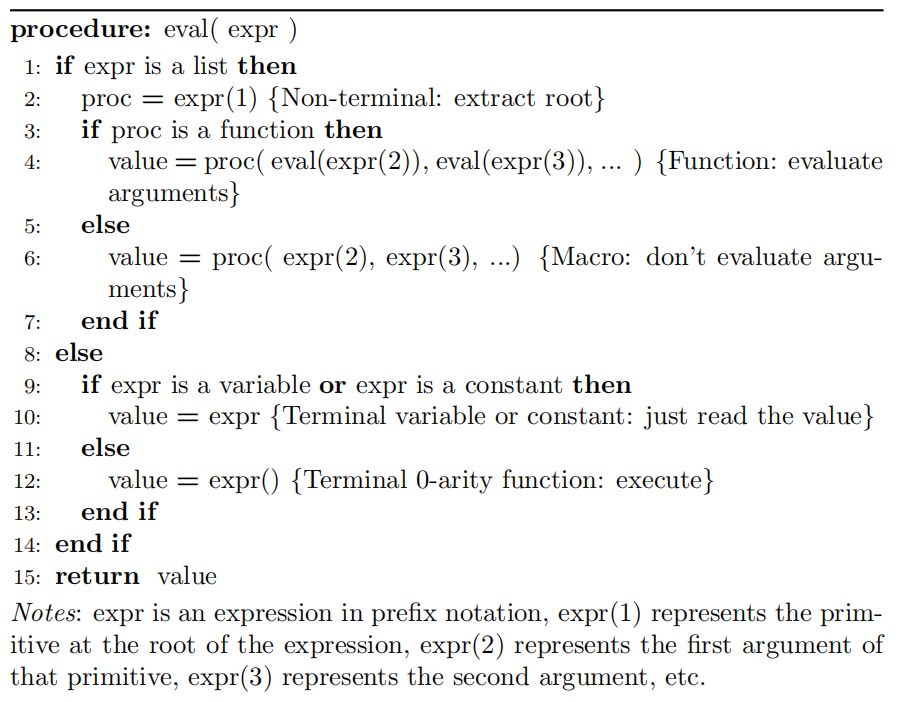
\includegraphics[width=14cm]{ia/pse-gp.png}
\caption{Algoritmo que evalúa un programa representado mediante un árbol sintáctico, Figura tomada de Jed Simson. (2017). Open-Source Linear Genetic Programming. : Faculty of Computing and Mathematical Sciences University of Waikato, Waikato, New Zealand.\cite{opensourceLGP}}
\label{fig:pse-gp} 
\end{figure}

\subsection{Selección} \index{Selección}

Debido a que los programas generados ya poseen un valor de aptitud se pueden utilizar los métodos descritos en la sección de selección para algoritmos genéticos \ref{selection:pse-ga} de este libro, así como cualquier otro método estándar de selección en algoritmos evolutivos. 

En este libro se sugiere analizar el comportamiento del algoritmo de programación genética con el método de selección elegido para determinar si es conveniente utilizar algún método con mayor o menor presión selectiva (A mayor presión selectiva mayor probabilidad hay de que los mejores individuos sean seleccionados como padres).
Como punto de inicio se puede utilizar el método de selección por torneo debido a su fácil implementación.

\subsection{El rol de los operadores de cruzamiento y mutación} \index{El rol de los operadores de cruzamiento y mutación}

Han existido discusiones de acuerdo a la importancia de los operadores de cruzamiento y mutación en los algoritmos evolutivos, un punto de vista tradicional nos indica que la mutación nos permite mantener diversidad en nuestra población y explorar el espacio de soluciones de nuestro problema, en cambio el cruzamiento nos permite ir mejorando la aptitud promedio de nuestra población y generar mejores individuos para llegar a la convergencia de nuestro algoritmo. La pregunta no es ¿Cruzamiento ó mutación?, lo ideal es usar ambas y encontrar el balance haciendo uso de los parámetros que como desarrolladores podemos modificar.

Si queremos analizar el comportamiento del uso de cruzamiento o mutación por separado se puede observar \cite{luke1997comparison} que en general el desempeño de algoritmos de programación genética que usan solo cruzamiento superan a aquellos que solo usan mutación y esta diferencia se hace más marcada al incrementar el tamaño de la población (Esto tiene sentido que ya que sin la mutación se requiere de una población grande para poseer suficiente diversidad para la convergencia exitosa del algoritmo).

Debido a que la representación de los individuos es muy distinta a la representación usada en los algoritmos genéticos los métodos de cruzamiento y mutación difieren a los presentados anteriormente.

\subsection{Cruzamiento} \index{Cruzamiento}

A continuación se presenta uno de los métodos más comunes para realizar el cruzamiento en un algoritmo genético.

\underline{Subtree crossover (Cruzamiento de un punto)}

Dados dos programas padres A y B se selecciona un punto de cruzamiento (un nodo) en cada padre $P_a$ y $P_b$ , para crear un nuevo programa se toma una copia del programa A y se reemplaza el subárbol cuya raíz es el nodo $P_a$ por el subárbol del padre B cuya raíz sea el punto $P_b$.
Esta técnica puede usarse para crear uno o dos hijos, el otro hijo tendría como base al padre B y se reemplazaría el subárbol cuya raíz es el nodo $P_b$ por el subárbol del padre A.

\begin{figure}[ht]
\centering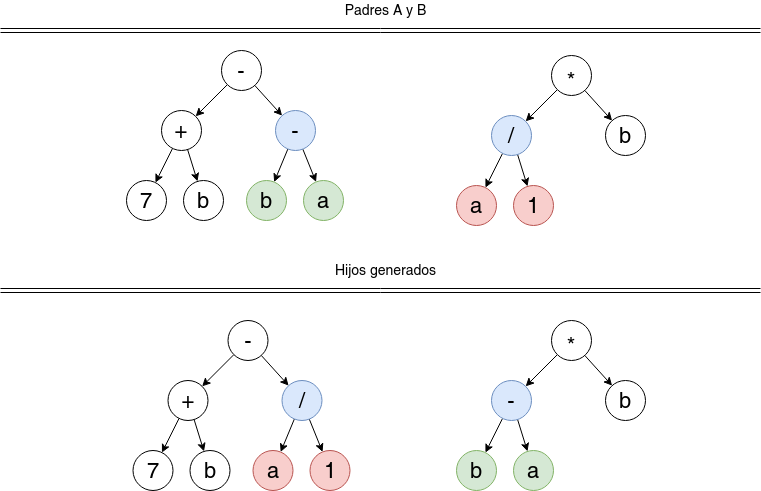
\includegraphics[width=12cm]{ia/GP - crossover.png}
\caption{Representación de la operación de cruzamiento, en la imagen se encuentran marcados con color azul los puntos de cruzamiento.}
\label{fig:GP - crossover} 
\end{figure}

Este es uno de los métodos más simples y existen versiones distintas del mismo, por ejemplo size-fair crossover es una variante que asegura que ambos subárboles utilizados para el cruzamiento tengan el mismo tamaño. Debido al alcance de este libro solo se mencionará este método de cruzamiento, si se desean conocer otras maneras de aplicar el operador de cruzamiento se recomienda leer el capítulo 5.3 del libro “A Field Guide to Genetic Programing” \cite{polilang08gp}.

\subsection{Mutación} \index{Mutación}

A continuación se presentan tres de los métodos más comunes para realizar la operación de mutación, de igual manera si se desean conocer más métodos se recomienda leer el capítulo 5.2 del libro “A Field Guide to Genetic Programing” \cite{polilang08gp}.

\underline{Point mutation (Node replacement mutation)}

Este método es muy similar al método Bit Flip mutation utilizado en los algoritmos genéticos, se selecciona un nodo en el árbol y se le cambia el valor, si este es un nodo de tipo terminal se cambia por otro nodo del mismo tipo, si el nodo es un nodo interno se cambia por otro nodo del conjunto de funciones que tenga el mismo número de argumentos.

\begin{figure}[ht]
\centering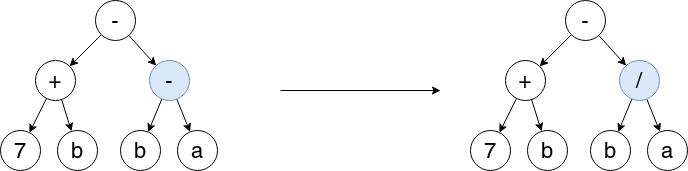
\includegraphics[width=14cm]{ia/GP -Point mutation.png}
\caption{Resultado del operador de mutación “point mutation”}
\label{fig:GP-Point-mutation} 
\end{figure}

\underline{Subtree mutation}

Se selecciona de manera aleatoria un subárbol dentro del individuo y este se reemplaza por un subárbol generado de manera aleatoria. La forma más básica de este método no limita la profundidad del nuevo subárbol, sin embargo existen variantes que restringen la profundidad del nuevo subárbol a ser del mismo tamaño o a ser como máximo 15\% (o algún otro porcentaje) más profundo que el subárbol original.

\begin{figure}[ht]
\centering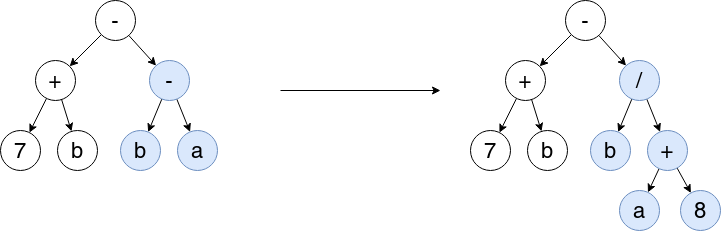
\includegraphics[width=14cm]{ia/GP -Subtree mutation.png}
\caption{Resultado del operador de mutación “subtree mutation”}
\label{fig:GP-Subtree-mutation} 
\end{figure}

\clearpage
\underline{Shrink mutation}

Se selecciona de manera aleatoria un subárbol dentro del individuo y este se reemplaza por un nodo terminal. El objetivo de este método de mutación es el de reducir el tamaño del programa.

\subsection{Construcción de un algoritmo de programación genética} \index{Construcción de un algoritmo de PG}

A continuación se presenta una tabla que resume los puntos que el desarrollador debe determinar o tomar en cuenta cuando construye un algoritmo de programación genética.


\begin{table}[ht!]
\centering
\caption{Parámetros y consideraciones en la construcción de un algoritmo de programación genética}

\begin{tabular}{|p{5cm}|p{9cm}|}
\hline
	Parámetros de la población & Tamaño de la población\\
\hline
	Representación de la población & Determinar el conjunto de funciones y el conjunto terminal (En el conjunto terminal hay que determinar los valores que puede tomar la constante aleatoria efímera $\Re$) \\
\hline
	Selección & Método de selección y parámetros del método seleccionado. Ej. Si se selecciona Selección por rango lineal se debe determinar el valor de Selective Pressure\\
\hline
	Cruzamiento & Método de cruzamiento.\\
\hline
	Mutación & Implementación de la mutación sobre nuestra población y  tasa de mutación\\
\hline
	Terminación & Determinar la condición de finalización\\
\hline

\end{tabular}
\end{table}

\FloatBarrier

\begin{center}
\line(1,0){420}
\end{center}

\textbf{Ejercicio de programación:}

En cualquier lenguaje de programación hacer un programa capaz de obtener una formula a partir de los datos de entrada y salida.


\includegraphics[width=4cm]{Pictures/github/progen.png}

(\url{https://github.com/amr205/FunctionDiscoverer---Genetic-Programming})

\section{Sistemas clasificadores (Learning classifier system)} \index{Sistemas clasificadores (Learning classifier system)} 

Los sistemas clasificadores buscan aprender un conjunto de reglas que se almacenan y se aplican para realizar la tarea de clasificación. Este tipo de algoritmo de clasificación utiliza las bases de los algoritmos evolutivos para el aprendizaje de las reglas (Por su funcionamiento también se considera un algoritmo de machine learning de aprendizaje supervisado o reforzado, si se quiere conocer a que se refiere esto se recomienda leer los primeros temas del capítulo Machine Learning).

\clearpage
\textbf{¿En qué consiste la tarea de clasificación?}

Dado un nuevo ejemplo de un elemento de un dominio específico ser capaz de etiquetarlo de manera correcta (asignarle un ejemplo).
Estos elementos o instancias comparten una estructura que contiene una serie finita de atributos.
Las etiquetas pueden ser de carácter discreto o continuo.

La tarea de clasificación puede servirnos para un espectro amplio de problemas, incluso nos puede servir para determinar qué acción realizar ante una situación determinada, el elemento del dominio sería la situación actual del entorno y la etiqueta la acción a realizar.

\subsection{Funcionamiento básico de las reglas en un LCS} \index{Funcionamiento básico de las reglas en un LCS}

Antes de analizar los tipos de LCS más comunes y su funcionamiento se describirá qué son las reglas y cómo determinan la clasificación de un ejemplo del dominio.

Para poder modelar el dominio se utilizan reglas, cada regla es parte de ese modelo. Cada regla está compuesta de una condición y una acción, la condición nos indica el valor que deberían tomar uno o más atributos, si esta condición se cumple la acción nos dice la clase a la cual corresponde el ejemplo. Supongamos que se tiene un problema donde cada ejemplo del dominio contiene 7 atributos que pueden tomar el valor de 0 o 1.

\begin{figure}[ht]
\centering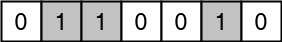
\includegraphics[width=6cm]{ia/LCS - Instancia.png}
\caption{Representación de una instancia que contiene 7 atributos donde cada uno de ellos puede tomar el valor de 0 o 1.}
\label{fig:LCS-Instancia} 
\end{figure}

Como se mencionó anteriormente la condición de una regla contiene los valores esperados en uno o más atributos (se suelen preferir reglas con menos atributos ya que son más generales, más adelante en este capítulo se verá cómo se favorecen este tipo de reglas), estas reglas suelen ser descritas como una sentencia condicional, a continuación se presentan reglas aplicadas sobre la instancia anterior para demostrar de manera visual su comportamiento.

\begin{figure}[ht]
\centering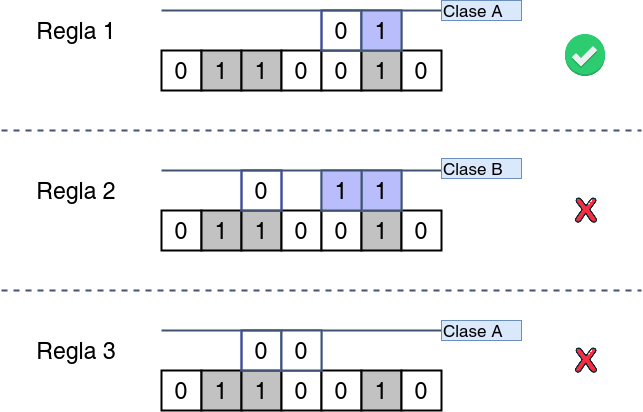
\includegraphics[width=11cm]{ia/LCS - Regla.png}
\caption{Reglas diferentes siendo aplicadas a una misma instancia.}
\label{fig:LCS-Regla} 
\end{figure}

En la figura \ref{fig:LCS-Regla} se puede observar que la única regla cuya condición se cumple es la regla 1 por ende la acción de esta regla indica que pertenece a la clase A. Si hubiera varias reglas que coincidieran la predicción estaría basada en la clase con mayor número de reglas cuya condición se cumpliera.
Ejemplo: Si para una instancia 5 reglas coinciden, 3 de ellas reglas con acción clase A y 2 con acción clase B, la clase que a predecir sería la clase A.

Esta explicación de cómo se utilizan las reglas para clasificar se retomará más adelante en el capítulo, en este momento se espera que el lector entienda su funcionamiento básico para observar la utilidad del algoritmo.

\FloatBarrier
\subsection{Tipos de LCS} \index{Tipos de LCS}

Los tipos más comunes de LCS que utilizan algoritmos evolutivos son LCS estilo Pittsburgh \cite{LCS_smith} y el estilo Michigan \cite{HOLLAND1978313}, estos dos estilos fueron contemporáneos. Actualmente LCS estilo Pittsburgh siguen siendo utilizados, sin embargo el estilo Michigan de LCS se ha convertido en el estándar \cite{SOW_LCS_SURVEY}. 

El estilo Pittsburgh usa como único elemento de adaptación un algoritmo genético, cada individuo de la población es un conjunto de reglas que se usan para la clasificación, es decir cada individuo es una solución completa al problema de clasificación.

El estilo Michigan utiliza elementos de aprendizaje reforzado en conjunto con un algoritmo genético cuyos individuos son reglas, este algoritmo se utiliza para descubrir nuevas reglas y es altamente elitista.
En este libro nos centraremos en el estilo Michigan debido a que actualmente es el estándar de los LCS que usan algoritmos evolutivos, además en este libro ya se cubrió el tema de algoritmos genéticos y se espera que el lector de este libro sea capaz de implementar un LCS estilo Pittsburgh haciendo uso de los conocimientos adquiridos en la sección \ref{section:Algoritmos-geneticos} (Algoritmos genéticos).

\begin{figure}[ht]
\centering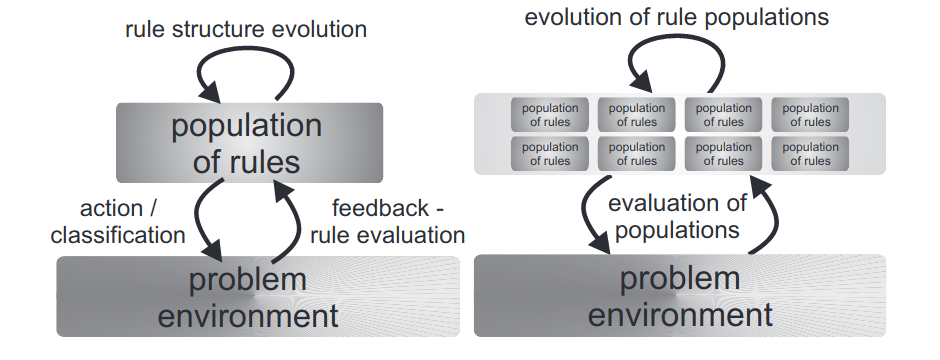
\includegraphics[width=12cm]{ia/comp-lcs.png}
\caption{Comparación entre el uso de algoritmos genéticos en los dos estilos (Pittsburgh-Derecha, Michigan-Izquierda), En el estilo Michigan un set de reglas evoluciona, en cambio en el estilo Pittsburgh poblaciones formadas por conjuntos de reglas compiten de una manera tradicional (basada fuertemente en el funcionamiento de los algoritmos genéticos). Figura tomada de Bacardit, J., Bernadó-Mansilla, E., and Butz, M.V. (2007). Learning Classifier Systems: Looking Back and Glimpsing Ahead. IWLCS. \cite{LCS_LBGA}}
\label{fig:comp-lcs} 
\end{figure}

\subsection{Mecanismos principales en un LCS} \index{Mecanismos principales en un LCS}

Este libro se centrará en el estilo Michigan, a partir de este punto se sobreentiende que el estilo que se está describiendo es este. Antes de presentar los componentes principales que contiene un LCS se describirán los mecanismos principales de un LCS con la finalidad de que sea más fácil identificar la finalidad de cada componente.

\clearpage
\textbf{Discovery o “descubrimiento”}

Este componente se refiere a la creación o el descubrimiento de nuevas reglas que no se encuentren actualmente en nuestra población, idealmente estas reglas serán mejores para solucionar el problema de clasificación. La forma más común de realizar este mecanismo es mediante un algoritmo genético \cite{UrbanowiczLCS}. El funcionamiento de este algoritmo genético es el descrito en la sección \ref{section:Algoritmos-geneticos}(Algoritmos genéticos) de este libro.

\textbf{Learning o aprendizaje}

El aprendizaje, en el contexto de la inteligencia artificial puede ser descrito como la mejora en el desempeño de una tarea en un ambiente a través de la adquisición de conocimiento, resultado de la experiencia en dicho ambiente \cite{rug01_000857792}. 

Como se verá posteriormente a mayor detalle en este capítulo cada regla que se encuentra dentro de la población tiene un conjunto de parámetros asociados, estos parámetros son actualizados en cada iteración mediante el mecanismo de aprendizaje.

El tipo de aprendizaje usado comúnmente en un LCS es aprendizaje reforzado, en este el agente interactúa con el ambiente y recibe una recompensa o penalización si se desempeña en este (el ambiente) de manera correcta o incorrecta respectivamente (asignación de créditos, “credit assignment”). Otro tipo de aprendizaje que puede usarse en un LCS es el aprendizaje supervisado, aquí durante el proceso de aprendizaje cada instancia es acompañada por la etiqueta de la clase a la cual pertenece, aquí los parámetros de las reglas son actualizados dependiendo de si la regla pudo clasificar de manera correcta o no la instancia.

Dentro del estilo Michigan existen diferentes implementaciones, estas implementaciones determinan el estilo de aprendizaje utilizado y los parámetros asociados a las reglas.

\subsection{Componentes y procesos de un LCS con aprendizaje reforzado} \index{Componentes y procesos de un LCS con aprendizaje reforzado}

\begin{figure}[ht]
\centering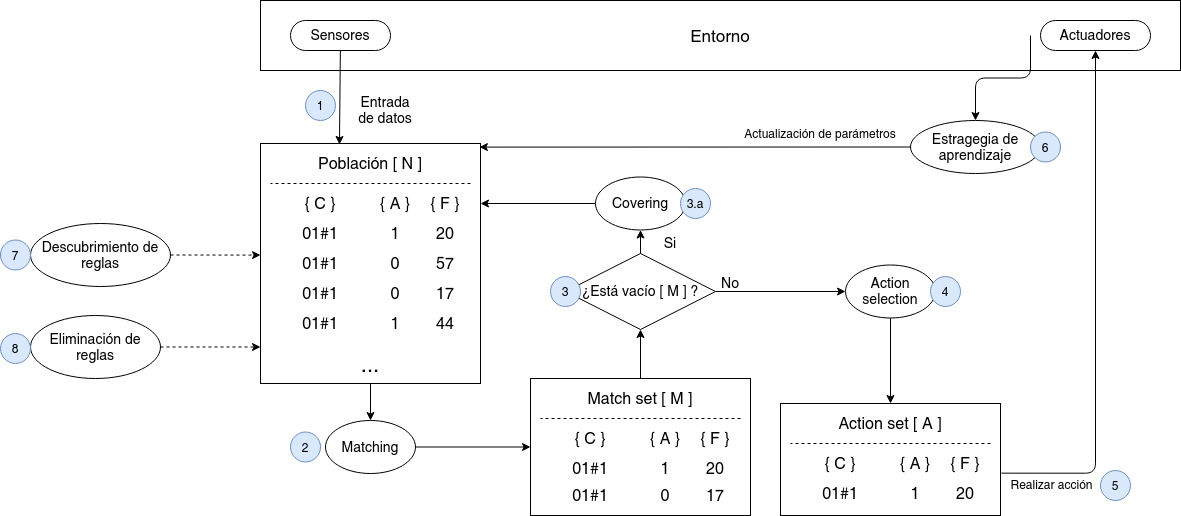
\includegraphics[width=15cm]{ia/LCS-RL.jpg}
\caption{Representación del proceso y los componentes que forman parte de un LCS con aprendizaje reforzado, en la figura cada elemento de la población de reglas contiene tres elementos: {C} el clasificador, {A} la acción correspondiente, { F } la aptitud (fitness).}
\label{fig:LCS-RL} 
\end{figure}

En la figura \ref{fig:LCS-SL} he tratado de representar el proceso que sigue un LCS con aprendizaje supervisado, a continuación describiré los diferentes elementos presentes en la figura.

\clearpage
\textbf{Environment o entorno}

 el elemento con el cual nuestro agente interactúa, el agente contiene sensores que nos permiten obtener información y actuadores que nos permiten modificar el entorno. Para entenderlo propongo el siguiente ejemplo: Tenemos un programa que juega baseball, mediante los sensores recibe la velocidad de la pelota,su distancia, y el ángulo de la misma, y mediante los actuadores puede determinar la velocidad y el ángulo con el cual el debe mover el bate.

\textbf{Población de reglas}

Este set contiene las reglas (clasificadores) que nos ayudan a realizar la tarea de clasificación. 

Como se ve en la figura  \ref{fig:LCS-Regla}, el cuerpo de la regla o condición \{ C \} no contiene un modelo, sino una parte del mismo, mediante un conjunto de reglas se puede modelar el problema.

Los caracteres que forman el cuerpo de la regla no están limitados a 0 y 1, dependiendo de cómo se forma el genotipo de las instancias del dominio del problema se formará de igual manera la regla. En la literatura se suele utilizar \# para denotar el “wildcard”, este elemento de la regla no se considerará para el proceso de matching, si representamos las tres reglas presentes en la figura \ref{fig:LCS-Regla} usando \# como wildcard se verían de la siguiente manera: \#|\#|\#|\#|0|1|\#, \#|\#|0|\#|1|1|\#,  \#|\#|0|0|\#|\#|\#.

Además del cuerpo de la regla, en LCS con aprendizaje reforzado, cada regla tiene asociada la acción \{ A \} que se realizará en el entorno, esta acción puede estar compuesta de un solo valor o un conjunto de valores, estos valores no están limitados al tipo binario y la forma está determinada por los valores que esperan los actuadores de nuestro agente. Por poner un ejemplo supongamos que nuestro agente debe manejar un dron y espera dos valores, un primer valor entero que especifique hacia que dirección (0-Adelante, 1-Atrás, 2-Izquierda, 3-Derecha) y un segundo valor flotante que detalle la velocidad con la que debe moverse.
Además de estos dos elementos cada regla tiene asociado un valor de aptitud \{ F \} y otros valores (que dependen de la implementación específica del LCS) llamados parámetros que nos sirven para realizar el proceso de aprendizaje y descubrimiento de reglas.

\textbf{Matching}

Es el proceso mediante el cual se seleccionan las reglas cuya condición satisface a la instancia en la iteración actual del proceso de aprendizaje. La Figura \ref{fig:LCS-Regla} muestra este proceso siendo aplicado sobre una instancia. Aquellas reglas cuya condición sea satisfecha pasan al conjunto de elementos llamados “match set” [ M ].

\textbf{Covering}

Si el match set [ M ] se encuentra vacío se realiza el siguiente proceso, se seleccionan un subconjunto de las características de nuestra instancia actual, el resto de elementos se llenan con wildcards para formar el cuerpo de una nueva regla, se le asigna una acción al azar y se inicializan con el promedio de los valores de la población. El número de wildcards está determinada por un valor $p_\#$ determinado por el programador.

Comúnmente los LCS inician con un conjunto de reglas [ N ] vacío (No en todas las implementaciones), por lo cual este proceso nos ayuda también a inicializar las reglas del LCS.

\begin{figure}[ht]
\centering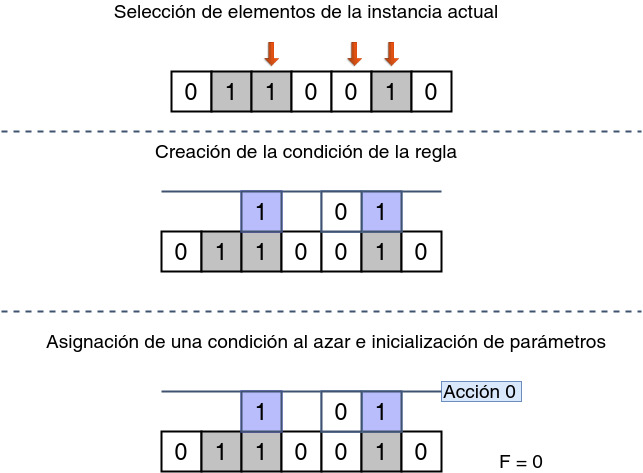
\includegraphics[width=13cm]{ia/LCS - Covering.jpg}
\caption{Representación visual del proceso de covering.}
\label{fig:LCS - Covering} 
\end{figure}

\FloatBarrier
\textbf{Action selection}

Durante este proceso se determina la acción que se realizará en el entorno y se forma el action set [ A ], la forma de realizar este proceso depende altamente de la implementación.

\textbf{Estrategia de aprendizaje}

Tras realizar la acción en nuestro entorno se nos devuelve un valor de recompensa P, usando este valor se modificarán los parámetros de las reglas, los parámetros y la manera en la que se modifican dependen de la implementación.

\textbf{Descubrimiento de reglas}

Como se mencionó anteriormente la manera más común de realizar esta parte del proceso en LCS estilo Michigan es mediante el uso de un algoritmo genético, este algoritmo genético suele ser altamente elitista por lo cuál solo una o dos reglas nuevas se añaden en cada iteración del proceso de aprendizaje. Los detalles del algoritmo como el tipo de cruzamiento, mutación y selección son dependientes de la implementación.

\textbf{Eliminación de reglas}

En los LCS se trata de mantener un número de reglas constante, en esta parte del proceso se eliminan las reglas con menor valor de aptitud hasta que el número de reglas sea igual o menor al límite establecido.

Algunas implementaciones de LCS pueden contener algunos componentes extras como el proceso de subsumption que se encarga de eliminar reglas específicas cuyo valor de aptitud sea menor o igual que el de una regla más generalizada.

\clearpage
\subsection{ZCS (LCS con aprendizaje reforzado)}
\begin{figure}[ht]
\centering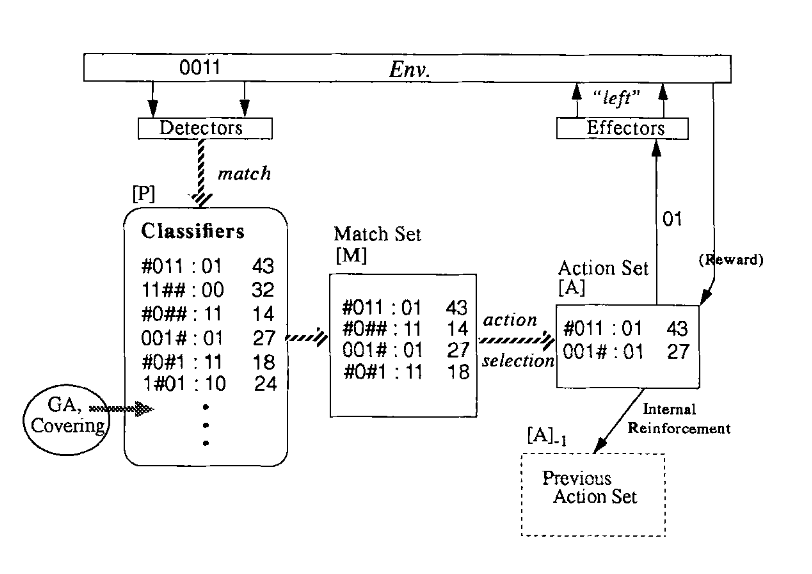
\includegraphics[width=12cm]{ia/zcs.png}
\caption{Representación del sistema clasificador ZCS. Figura tomada de Wilson, Stewart. (1994). ZCS: A zeroth level classifier system. Evolutionary Computation. 2. 10.1162/evco.1994.2.1.1. \cite{wilste_zcs}}
\label{fig:zcs} 
\end{figure}

El sistema clasificador “Zeroth-level” System Classifier (ZCS) fue introducido por Wilson \cite{wilste_zcs}, este LCS toma como base los trabajos de Holland y utiliza aprendizaje reforzado como estrategia de aprendizaje. Como se puede observar en la figura \ref{fig:zcs} la arquitectura del sistema clasificador ZCS es muy similar a la arquitectura presentada en la Figura \ref{fig:LCS-RL}. 

\textbf{Funcionamiento del ZCS}

El ZCS comienza con una población de reglas [ P ] generada de manera aleatoria, el valor inicial de aptitud que toman las reglas es el valor $S_0$. En diversas publicaciones el valor de aptitud es llamado fitness o strength.A continuación se describe una iteración en el proceso de aprendizaje en un ZCS \cite{cadrik_zcs}:

\begin{enumerate}
\item Se obtiene la información de entrada del entorno 
\item Se realiza el proceso de matching para obtener el match set [ M ]. \textbf{(matching)} 
\item Si [ M ] se encuentra vacío se activa el mecanismo de covering (el único parámetro en ZCS que se requiere para cada regla es el valor de aptitud) añadiendo una nueva regla a la población, eliminando la regla con menor aptitud en la población de reglas y regresando al paso 2. \textbf{(covering)}.
\item Usando el método de ruleta (descrito en la sección \ref{selection:pse-ga}) se selecciona una regla R. Se copia el valor del action set [ A ] al conjunto [ A-1 ], Se vacía el action set [ A ] y cada regla que contenga la misma acción que la regla R se añade al action set [ A ]. 
\textbf{(action selection)}
\item Se actualiza el valor de aptitud de cada regla en [ M ] que no se encuentre en [ A ] de acuerdo a la siguiente fórmula. (empieza la estrategia de aprendizaje)

\begin{equation}
fitness_j=fitness_j-fitness_j*\tau
\end{equation}

$\tau$ es un parámetro (no un parámetro de una regla sino del LCS) determinado por el programador o usuario, el dominio de $\tau$ es (0,1).

\item Se calcula la siguiente variable para cada regla que se encuentra en [ A ]

\begin{equation}
value_j = fitness_j * \beta
\end{equation}

$\beta$ es un segundo parámetro cuyo valor tiene el mismo dominio que $\tau$. Posteriormente se actualiza el valor de aptitud de las reglas en [ A ] de acuerdo a la siguiente fórmula.

\begin{equation}
fitness_j=fitness_j-value_j
\end{equation}

Se guarda temporalmente el valor “Bucket” B definido de la siguiente manera:

\begin{equation}
B = \sum_{j=1}^{b}value_j
\end{equation}
\item Se ejecuta la acción en el entorno y se obtiene un valor de recompensa reward. Usando este valor se actualiza el valor de aptitud de las reglas en [ A ] de la siguiente manera:

\begin{equation}
fitness_j=fitness_j+\beta*\frac{reward}{|A|}
\end{equation}

En la fórmula anterior | A | es la cardinalidad del conjunto [ A ]
\item Por último para terminar la estrategia de aprendizaje se actualiza el valor del conjunto [A-1]:

\begin{equation}
fitness_j = fitness_j +\gamma*\frac{B}{|A-1|} 
\end{equation}

Donde $\gamma$ es un parametro del LCS cuyo valor esta entre 0 y 1.

\textbf{(termina la estrategia de aprendizaje)}

\item El siguiente paso es el proceso de descubrimiento de reglas, Wilson \cite{wilste_zcs} no describe los detalles del algoritmo genético, sin embargo C{\'a}drik y Mach \cite{cadrik_zcs}, mencionan que se usa un algoritmo genético con selección por ruleta, cruzamiento de un punto y para la mutación cada carácter del genotipo tiene una probabilidad pm de mutar tomando uno de los tres valores posibles 0,1 y \# (siendo \# un wildcard). Este algoritmo es altamente elitista, por ende solo se generan dos reglas nuevas que se añaden al conjunto [ P ] \textbf{(descubrimiento de reglas)}.

\item Para mantener constante el número de reglas en la población [ P ] se eliminan dos reglas de la población, preferiblemente aquellas con un valor bajo de aptitud. \textbf{(eliminación de reglas)}

\end{enumerate}

\clearpage
\subsection{Componentes y procesos de un LCS con aprendizaje supervisado} \index{Componentes y procesos de un LCS con aprendizaje supervisado}

\begin{figure}[ht]
\centering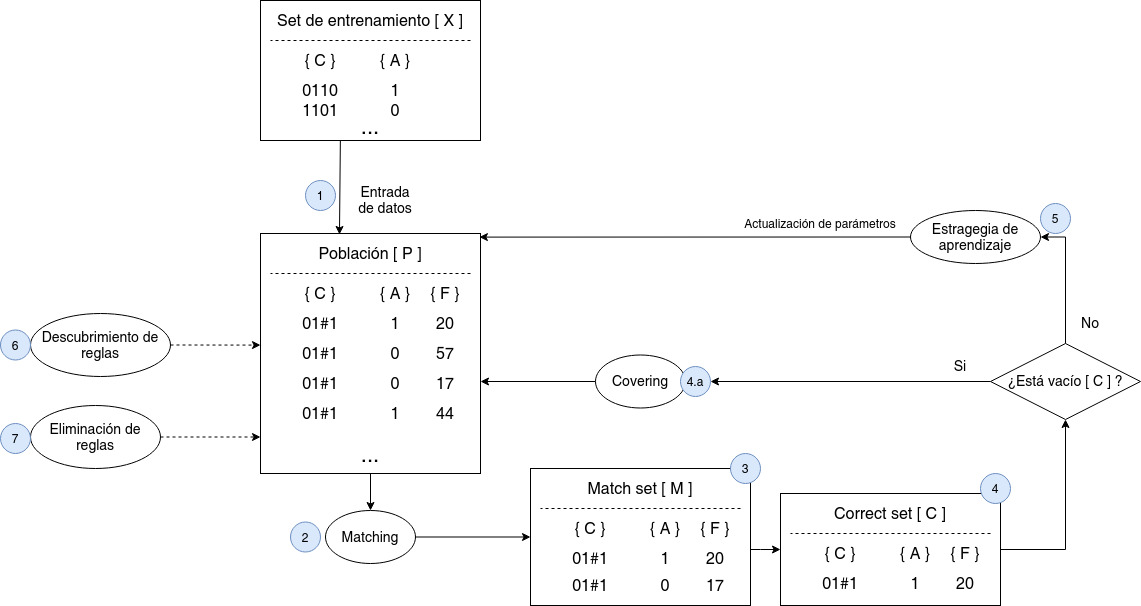
\includegraphics[width=14.5cm]{ia/LCS-SL.jpg}
\caption{Representación del proceso y los componentes que forman parte de un LCS con aprendizaje supervisado, en la figura cada elemento de la población de reglas contiene tres elementos: {C} el clasificador, {A} la acción correspondiente, { F } la aptitud (fitness).}

\label{fig:LCS-SL} 
\end{figure}

Podemos observar que el LCS con aprendizaje supervisado no difiere tanto en comparación a un LCS con aprendizaje reforzado, la principal diferencia radica en la ausencia del entorno, aquí para el proceso de aprendizaje se requiere de un set de entrenamiento que contiene ejemplos de nuestro dominio con su etiqueta correspondiente.

Para evitar ser repetitivo no mencionaré los componentes que también se encuentran en una arquitectura LCS con aprendizaje reforzado y me centraré en las diferencias.

En lugar de un action set tenemos un correct set [ C ] este set contiene todos los elementos del match set [ M ] que contengan la misma etiqueta (acción) que la instancia de la iteración actual.

Para el proceso de aprendizaje ya no es necesario interactuar con el entorno, una vez creados el match set [ M ] y correct set [ C ] se puede proceder a la actualización de parámetros, los parámetros y la manera en la que se actualizan es dependiente de la implementación.

Otra diferencia es el momento en el que el mecanismo de covering se activa, en los LCS con aprendizaje reforzado se utilizaban cuando el match set [ M ] estaba vacío, sin embargo en este tipo de LCS se activa el mecanismo cuando el correct set [ C ] no tiene ningún elemento, además de esto la clase que toma la regla creada por el covering debe tener la misma clase que la instancia de la iteración actual.

\subsection{UCS (LCS con aprendizaje supervisado)} \index{UCS (LCS con aprendizaje supervisado)}

El clasificador UCS deriva del XCS (un clasificador basado en la exactitud o “accuracy” en inglés, con aprendizaje reforzado), a diferencia del clasificador XCS adapta sus componentes para utilizar aprendizaje supervisado.

\textbf{Parámetros de las reglas o clasificadores en UCS}

Estos parámetros tendrán que ser actualizados durante el proceso de aprendizaje: exactitud o “accuracy” \{ acc \}, aptitud o “fitness” \{ F \}, tamaño del correct set o “correct set size” \{ cs \}, “numerosity” \{ num \} y experiencia o “experience” \{ exp \}.

La aptitud y exactitud de la regla nos sirve para determinar la calidad de la misma, el tamaño del correct set es el tamaño promedio del correct set [ C ] en los cuales ha participado, el valor de “numerosity” indica cuantas veces se encuentra presente la misma regla en la población [ P ] y la experiencia nos indica cuantas veces esta regla ha pertenecido a algún match set [ M ]. \cite{orriols2006further}.

A continuación se describe una iteración en el proceso de aprendizaje en un clasificador UCS:
\begin{enumerate}
\item Se obtiene una instancia xi del set de entrenamiento [ X ] junto con su clase correspondiente.
\item Se realiza el proceso de matching para obtener el match set [ M ]. \textbf{(matching)} 
\item Se obtienen todas las reglas del match set [ M ] que posean la misma clase o etiqueta de la instancia actual $x_i$ para formar el correct set [ C ].
\item Si [ C ] se encuentra vacío se activa el mecanismo de covering, los parámetros son inicializados de la siguiente manera: exp = 1, num = 1, cs = 1, acc = 1 and F = 1. Después de añadir la nueva regla se elimina la regla con menor valor de aptitud. \textbf{(covering)}.
\item Ahora se van a actualizar los valores de los parámetros de las reglas:
Se aumenta el valor de experiencia \{ exp \} de todas las reglas en el match set [ M ], y se actualiza el valor de exactitud de las reglas de acuerdo a si estas pertenecen o no al correct set [ C ]:

\begin{equation}
acc=\frac{clasificacionses_{correctas}}{exp}
\end{equation}

Para poder lograr actualizar los parámetros yo propongo el aplicar las siguientes fórmulas en el orden mostrado, primero empezamos aplicando las siguientes fórmulas sobre todos los elementos del match set [ M ]:

\begin{equation}
exp_j=exp_j+1
\end{equation}

\begin{equation}
acc_j=acc_j*\frac{exp_j-1}{exp_j}
\end{equation}

Ahora actualizamos los siguientes valores de las reglas presentes en el correct set [ C ]:

\begin{equation}
acc_j=acc_j+\frac{1}{exp_j}
\end{equation}

\begin{equation}
css_j=\frac{css_j*((acc_j*exp_j)-1)+|C|}{exp_j}
\end{equation}

Por último actualizamos el valor de aptitud de todos los elementos en el match set [ M ]

\begin{equation}
F=(acc_j)^{v}
\end{equation}

Donde v en la fórmula anterior suele tener el valor v = 10.
\textbf{(estrategia de aprendizaje)}
\item El siguiente paso es el proceso de descubrimiento de reglas, se puede utilizar un algoritmo genético con selección por ruleta, cruzamiento de un punto y para la mutación cada carácter del genotipo tiene una probabilidad pm de mutar tomando uno de los tres valores posibles 0,1 y \# (siendo \# un wildcard). Este algoritmo es altamente elitista, por ende solo se generan dos reglas nuevas que se añaden al conjunto [ P ] (descubrimiento de reglas). Los iniciales que toman los parámetros son los siguientes: exp = 0, num = 1, cs = (csp1 + csp2)/2 (Donde p1 y p2 son los padres), acc = 1 y  F=1. \textbf{(descubrimiento de reglas)}
\item Para mantener constante el número de reglas en la población [ P ] se eliminan dos reglas de la población, preferiblemente aquellas con un valor bajo de aptitud. \textbf{(eliminación de reglas)}
\end{enumerate}

\subsection{Conclusión de los LCS} \index{Conclusión de los LCS}

Actualmente gracias a técnicas de Deep Learning se han logrado resolver tareas de clasificación muy complejas, por lo tanto el uso de los LCS ha disminuido, sin embargo los LCS se han aplicado exitosamente para resolver fenómenos biológicos. Es interesante observar como John Holland incursionó en el campo de los algoritmos genéticos y luego usando ideas propias del machine learning desarrolló un algoritmo híbrido que utiliza algoritmos genéticos como un componente del sistema. En mi opinión una de las ventajas de estos sistemas es la facilidad con la cuál puede ser interpretada una regla, sin embargo mientras más grande es el tamaño de la población se vuelve más confuso el interpretar el sistema como un conjunto.

En este tema solo se vieron dos implementaciones específicas de los LCS y existen muchas otras que podrían adaptarse a algún problema que se quiera resolver, por estás razones colocaré aquí el link del trabajo de Urbanowicz \cite{UrbanowiczLCS}. (\url{https://www.researchgate.net/publication/26850330_Learning_Classifier_Systems_A_Complete_Introduction_Review_and_Roadmap})


\subsection{Panorama actual de los algoritmos evolutivos} \index{Panorama actual de los algoritmos evolutivos}

La investigación y el desarrollo de los algoritmos evolutivos lleva más de 50 años por lo cual hoy en día existen algoritmos robustos que permiten solucionar diversos problemas. Han demostrado que pueden dar soluciones a problemas difíciles, sin embargo a pesar de tener resultados en el ámbito académico se puede observar que en las industrias ha tenido menor éxito. Las nuevas tendencias apuntan al uso de algoritmos híbridos que combinen diversos paradigmas para solucionar problemas más complejos \cite{slossEA}.

En lo personal considero que los algoritmos evolutivos si tienen aplicaciones importantes como su uso en la parametrización de dispositivos y programas, es importante observar las ventajas que nos provee cada tipo de algoritmo para poder identificar aquellos problemas que puedan ser resueltos utilizando un determinado tipo de programa. (La posibilidad de encontrar explorar un espacio de soluciones y encontrar una buena solución haciendo uso de una función de aptitud me parece una de las grandes ventajas ya que existen problemas que no pueden utilizar un algoritmo de optimización basado en el uso de gradientes).

\chapter{Inteligencia Artificial Simbólica} \index{Inteligencia Artificial Simbólica}

\section{Introducción al capítulo} \index{Introducción al capítulo}

A continuación se presentan tres de las implicaciones principales de los sistemas de inteligencia artificial simbólica \cite{flasinski2016symbolic}:
\begin{itemize}
\item Un modelo que represente un sistema inteligente puede ser definido de manera explícita.
\item El conocimiento de estos modelos puede ser representado de manera simbólica (Estos símbolos suelen ser de alto nivel por lo cual pueden ser interpretados por humanos, algunos ejemplos son el uso de grafos, fórmulas lógicas, fórmulas matemáticas, etc)
\item Las operaciones mentales y cognitivas pueden ser descritas de manera formal utilizando las estructuras que corresponden al conocimiento descrito en nuestros modelos.
\end{itemize}

En los modelos de inteligencia artificial se asume que muchos aspectos de la inteligencia pueden ser simulados mediante la manipulación de símbolos.

\section{Ventajas y desventajas del paradigma simbólico} \index{Ventajas y desventajas del paradigma simbólico}

Entre las ventajas de estos sistemas se encuentran las siguientes \cite{GARNELO201917}:
\begin{itemize}
\item \textbf{Interpretabilidad:} Debido al uso de símbolos (generalmente de alto nivel, como nodos, predicados, etc) y la naturaleza de las operaciones realizadas con ellos (transición entre estados válidos, operaciones de inferencia, etc) es fácil entender el funcionamiento de los sistemas y la manera en la cual llegan a los resultados obtenidos.
\item \textbf{Generalización:} Las representaciones simbólicas de alto nivel pueden permitir generalización.
\item \textbf{Eficiencia de los datos:} Este paradigma a diferencia de otros no requiere una gran cantidad de datos (un ejemplo de lo contrario son muchos algoritmos del paradigma conexionista), el uso de los símbolos también permite que estos puedan ser reutilizados en otros escenarios.
\end{itemize}

Dentro de las principales desventajas es el hecho de que el conocimiento no suele ser aprendido sino diseñado de manera “manual”, otro punto a considerar es el hecho de que hay conocimiento demasiado complejo como para ser plasmado de esta manera. Por lo anteriormente mencionado no hubo mucho avance con este paradigma en el reconocimiento de imágenes y el procesamiento del lenguaje natural.

\section{Orígenes} \index{Orígenes}

Uno de los primeros programas basados en el uso de reglas lógicas fue “Logic Theorist” creado por Allen Newell, Herbert A. Simon y Cliff Shaw en 1956, este programa eventualmente demostró 38 de los primeros 52 teoremas del trabajo Principia Mathematica. 

El trabajo realizado por Newell, Simon y Shaw precedió a la conferencia de Dartmouth, a pesar de que ellos ya habían realizado un programa que utilizaba uno de los paradigmas más importantes de la inteligencia artificial simbólica (Simulación cognitiva) parece que nadie salvo ellos se dieron cuenta de la importancia de su trabajo a largo plazo \cite{mccorduck2004machines}.

La idea de usar la lógica como representación de la información en un programa se le atribuye a John McCarthy por su propuesta del “advice taker” en 1958. El programa propuesto por John McCarthy era un programa hipotético, J. Alan Robinson en 1963 desarrolló una manera de implementar deducción en una computadora mediante el algoritmo de resolución y unificación, sin embargo las implementaciones de estos algoritmos resultaban en programas que tardaban demasiadas iteraciones en dar resultados.

En 1970 se obtuvieron mejores resultados al reducir la lógica al uso de cláusulas de Horn, de esta manera se desarrollaron mejores algoritmos de deducción y se creó el lenguaje de programación Prolog (Un lenguaje de programación declarativo basado en la programación lógica).

\section{Clasificación} \index{Clasificación}
Existen diversos acercamientos a la inteligencia artificial simbólica que cumplen con las características presentadas al inicio de este capítulo, a continuación se presenta una pequeña descripción de cada uno de ellos \cite{flasinski2016symbolic}:

\begin{itemize}
\item \textbf{Simulación cognitiva:} Se basa en simular habilidades cognitivas del ser humano (resolución de problemas, razonamiento, aprendizaje) mediante la definición de algoritmos que implementen la heurística. Por lo tanto, en el diseño de estos algoritmos se trata de descubrir conceptos y reglas que nos permiten resolver problemas. Anteriormente se mencionó que el trabajo de Newell, Simon y Shaw (Logic Theorist) incorporaba este acercamiento de manera exitosa.
\item \textbf{Acercamiento basado en lógica:} John McCarthy fue el precursor de este tipo de sistemas ya que aseguraba que un sistema inteligente debería de estar basado en sistemas formales de razonamiento lógica en lugar de “simuladores” de procesos mentales basados en algoritmos heurísticos. De esta manera el conocimiento podía ser representado mediante reglas lógicas y un programa universal (un programa dedicado a resolver problemas mediante la inferencia) se encargaría de encontrar la solución.
\item \textbf{Representación de conocimiento basado en reglas:} Newell y Simon continuaron su investigación en modelos cognitivos y en 1972 propusieron sistemas basados en la memoria a corto y largo plazo. La memoria a largo plazo (production memory) es representada por reglas simples (si .... entonces ...) y la memoria a corto plazo (working memory) contiene la información del entorno sobre el cual opera, continuamente monitorea los datos de la memoria a corto plazo para determinar si alguna regla de la production memory se cumple, en caso de que la condición de la regla sea satisfecha se ejecuta la acción de la regla que puede ser una conclusión, la adición de una regla a la memoria a largo plazo, una acción que permita interactuar con el entorno, etc.
Este acercamiento no tuvo tanto éxito, uno de sus programas más relevantes fue la creación de un sistema experto basado en reglas, estos sistemas expertos son una subclase de los sistemas expertos que se pueden producir usando el acercamiento basado en la lógica.
\item \textbf{Representación estructurada del conocimiento:} Este acercamiento se basa en la manipulación de estructuras que contienen conocimiento, estas estructuras pueden ser redes semánticas, marcos (frames), etc. 
Mediante el uso de estas estructuras se busca desarrollar programas capaces de  resolver problemas específicos.
\end{itemize}

De estos acercamientos yo considero que el más exitoso fue el de la programación lógica (o acercamiento basado en lógica), gracias a este acercamiento se desarrollaron los sistemas expertos que dieron lugar al boom de la inteligencia artificial (1980–1987), sin embargo es importante tener en cuenta las limitaciones, ventajas y desventajas de este tipo de sistemas.

Este capítulo se centrará en el acercamiento basado en lógica debido no solamente a ser el de mayor éxito, sino también por su base formal. 

\section{Simulación cognitiva} \index{Simulación cognitiva}

Como se mencionó anteriormente la simulación cognitiva se basa en simular habilidades cognitivas del ser humano mediante la definición de algoritmos que implementen la heurística. Vamos a profundizar un poco en su funcionamiento y luego exploraremos de manera simple el funcionamiento del programa “logic theorist”.

En la resolución de problemas partimos de un estado inicial que representa la situación actual del problema, mediante funciones de transición podemos pasar a otros estados (tomando el ejemplo del ajedrez estas funciones de transición serían todos los movimientos válidos) si estos estados son nuestra solución se les llama “goal states” en caso de que no lo sea son estados intermedios. Un espacio de estados está constituido por estos estados (inicial, intermedio y objetivo), se puede representar mediante un grafo, donde los nodos son los estados y los ejes son las transiciones entre los mismos.

En la simulación cognitiva podemos usar estos conceptos para generar soluciones, partiendo de un estado inicial se aplican funciones de transición para ampliar nuestro espacio de estados y buscar una nueva solución, aquí podemos observar que el espacio de estados crecería de manera exponencial en la búsqueda de soluciones por lo cual estos algoritmos suelen implementar heurística para cortar algunas de las ramas y reducir el espacio de búsqueda.

Ahora vamos a observar como el programa “logic theorist” utiliza estos conceptos para probar teoremas matemáticos:

Parte de un conjunto de teoremas, que es nuestro estado inicial.
Utiliza diferentes funciones de transición para expandir el espacio de estados, estas funciones pueden ser las siguientes:
\begin{itemize}
\item Método de reemplazo
\item Método de separación (modus ponendo ponens)
\item Método de encadenamiento
\end{itemize}

Estos métodos se aplican sobre teoremas que se quieren comprobar, utilizando los teoremas en nuestro estado actual, si alguno de estos métodos logra comprobar la veracidad de un teorema, este se añade a los teoremas comprobados ampliando así nuestro espacio de estados.

Logic theorist utiliza la heurística en el funcionamiento de estos métodos tomando los axiomas comprobados que sean más “prometedores” en la comprobación del teorema.

\section{Programación lógica} \index{Programación lógica}

Para explorar este acercamiento del paradigma simbólico vamos a partir de la pregunta ¿Qué es la razón?, la razón la capacidad de la mente humana de establecer relaciones entre ideas o conceptos y obtener conclusiones o formar juicios, este acercamiento busca simular o imitar esta facultad de la mente por medio del razonamiento lógico, dado un conjunto de juicios que mantienen relaciones lógicas entre sí (premisas) se puede deducir o inferir un nuevo juicio al que denominamos conclusión.

“La ciencia que estudia que tipos de esquemas de inferencia aseguran la validez de las conclusiones es la lógica” \cite{munoz2013introduccion}.

Mediante la lógica podemos representar el conocimiento y utilizarlo de tal manera que si las premisas son verdaderas, la conclusión también lo será.

\subsection{La lógica formal} \index{La lógica formal}

La lógica formal o lógica matemática estudia los principios y métodos que se emplean para diferenciar el razonamiento correcto del incorrecto.
Analicemos el siguiente razonamiento:

Si estoy corriendo entonces voy más lento\\
Estoy corriendo\\
-Por lo tanto: voy más lento

Este razonamiento podría parecer incorrecto debido a que sabemos que si corremos vamos más rápido, sin embargo la lógica formal estudia la lógica del razonamiento, si le asignamos letras a las distintas proposiciones podemos damos cuenta de que en realidad este razonamiento es correcto.

p: estoy corriendo \\
q: voy más lento

p → q\\
p \\
\line(1,0){50}\\
q

Podemos decir que esta inferencia posee validez formal

\subsection{Clasificación de la lógica} \index{Clasificación de la lógica}

La lógica tiene diversas subdivisiones, cada una con su propia semántica y sintaxis, algo importante es observar cómo cada una de las divisiones de la lógica expande la lógica del orden anterior, en consecuencia es más expresiva y por ende requiere de añadir más recursos o eliminar restricciones sobre el uso de los ya existentes \cite{munoz2013introduccion}.


\begin{figure}[ht]
\centering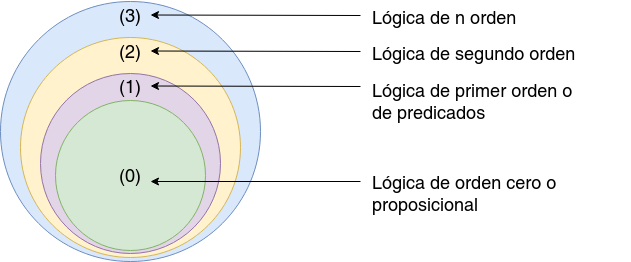
\includegraphics[width=8cm]{ia/Division in logic.png}
\caption{Representación de las diversas divisiones en la lógica.}

\label{fig:Division-in-logic} 
\end{figure}

\FloatBarrier
También se puede dividir la lógica en lógica clásica y no clásica, en la lógica clásica las fórmulas lógicas solo pueden tener dos valores (verdadero o falso), por eso se le llama cálculo bivalente, en la lógica no clásica las fórmulas pueden tomar más valores, un ejemplo es la lógica trivalente que además de los valores verdadero y falso contempla un tercer valor que no representa que el valor se desconoce o es incierto \cite{munoz2013introduccion}.

Existen otro tipo de lógicas que contemplan elementos como el tiempo, en el cual el valor de verdad depende del momento actual o en el que dio lugar.

\textbf{Nota: Diferencia entre lógica de predicados y cálculo de predicados}

Es común encontrar estos términos y preguntarse la diferencia entre los mismos, estos términos suelen usarse de manera intercambiable y representan lo mismo, cada cálculo o división de la lógica debe componerse de los siguientes elementos \cite{munoz2013introduccion}:

\begin{itemize}
\item La \textbf{semántica} de la lógica, el significado de cada uno de los elementos que la compone.
\item Una \textbf{sintaxis} que nos permita formar combinaciones correctas de los elementos primitivos . Mediante la definición de un conjunto de \textbf{reglas de formación} podemos definir como es una \textbf{fórmula bien} formada (fbf, otro término con el cual es probable encontrarse), de esta manera se puede determinar si la combinación de los elementos es correcta o no.
\item Un conjunto de \textbf{reglas de transformación} de carácter algorítmico que nos permitan ir de una fbf a otra, estas transformaciones deben asegurar la validez formal de las fórmulas lógicas.
\end{itemize}

En este tema veremos cómo podemos utilizar la lógica de primer orden para implementar un sistema experto, este programa emula las capacidades de tomar decisiones del ser humano, debido a que como se mencionó aquí los cálculos de la lógica se construyen sobre la lógica del orden anterior primero revisaremos la lógica de orden cero.

\subsection{Lógica de orden cero o proposicional} \index{Lógica de orden cero o proposicional}

La lógica proposicional es la más simple de los tipos de lógica y como su nombre indica está basada en sentencias o proposiciones, una \textbf{sentencia o proposición} es una oración capaz de tener un valor de verdad (verdadero o falso).

Mediante las proposiciones podemos representar información, ejemplo:

p: estoy corriendo\\
q: voy más rápido

Estas dos proposiciones contienen un solo elemento por lo cual son conocidas como \textbf{proposiciones atómicas o proposiciones simples} (También se les conoce como proposiciones primitivas).

Mediante el uso de conectores operadores lógicos podemos formar \textbf{proposiciones compuestas}, que nos muestran las relaciones entre las proposiciones, ejemplo (si llueve, entonces voy más rápido):

p → q\\

\textbf{Operadores lógicos}

A continuación se describirán los diferentes operadores lógicos y mediante el uso de tablas de verdad \footnote{ Una tabla de verdad, o tabla de valores de verdades, es una tabla que muestra el valor de verdad de una proposición compuesta, para cada combinación de verdad que se pueda asignar } se mostrará su comportamiento
(1 - Verdadero, 0 - Falso):

\clearpage
\underline{Negación ¬}

Cuando la variable es verdadera al negarla se convierte en falsa, y si es falsa, al negarla se hace verdadera.

\begin{tabular}{|l|l|}
\hline
	A &	¬A\\
\hline
	1 & 0\\
\hline
	0 & 1\\
\hline
\end{tabular}

\underline{Disyunción v}

Es falsa cuando ambas proposiciones son falsas.

\begin{tabular}{|l|l|l|}
\hline
	A	& B	& A v B\\
\hline
	1 & 1 & 1\\
\hline
	1 & 0 & 1\\
\hline
	0 & 1 & 1\\
\hline
	0 & 0 & 0\\
\hline
\end{tabular}

\underline{Conjunción $\Lambda$}

Solo es verdadera cuando ambas proposiciones son verdaderas.

\begin{tabular}{|l|l|l|}
\hline
	A	& B	& A $\Lambda$ B \\
\hline
	1 & 1 & 1\\
\hline
	1 & 0 & 0\\
\hline
	0 & 1 & 0\\
\hline
	0 & 0 & 0\\
\hline
\end{tabular}

\underline{Condicional →}

Solo es falsa cuando la primera proposición es verdadera y la segunda falsa.

\begin{tabular}{|l|l|l|}
\hline
	A	& B	& A → B \\
\hline
	1 & 1 & 1\\
\hline
	1 & 0 & 0\\
\hline
	0 & 1 & 1\\
\hline
	0 & 0 & 1\\
\hline
\end{tabular}

\underline{Bicondicional $\leftrightarrow$}

Solo es verdadera cuando ambas proposiciones tienen el mismo valor.

\begin{tabular}{|l|l|l|}
\hline
	A	& B	& A $\leftrightarrow$ B \\
\hline
	1 & 1 & 1\\
\hline
	1 & 0 & 0\\
\hline
	0 & 1 & 0\\
\hline
	0 & 0 & 1\\
\hline
\end{tabular}

Utilizando estas conectivas podemos representar conocimiento más complejo

Si es sábado o es domingo entonces saco a pasear a mi perro y desayuno hotcakes. \\
a: es sábado \\
b: es domingo \\
c: saco a pasear a mi perro \\
d: desayuno hotcakes

(a v b) → (c $\Lambda$ d)

Aquí quiero hacer notar el uso de la condicional, cuando no es sábado o domingo puede ser que saque a pasear a mi perro y desayune hotcakes, pero siempre que sea sábado o domingo voy a sacar a mi perro a pasear y desayunar hotcakes.

Ahora vamos a dar las reglas de formación para crear fórmulas bien formadas usando la notación de Backus-Naur (BNF):

< Fórmula > ::= ProposiciónAtómica\\
\phantom{.} \quad	\quad \quad \quad| ¬ < Fórmula >\\
\phantom{.} \quad	\quad \quad \quad| < Fórmula > $\Lambda$ < Fórmula >\\
\phantom{.} \quad	\quad \quad \quad| < Fórmula > v < Fórmula >\\
\phantom{.} \quad	\quad \quad \quad| < Fórmula > → < Fórmula >\\
\phantom{.} \quad	\quad \quad \quad| < Fórmula > $\leftrightarrow$ < Fórmula >\\
\phantom{.} \quad	\quad \quad \quad| ( < Fórmula > )

\textbf{Tipos de fórmulas bien formadas en lógica proposicional}

\underline{Tautología:} es una fbf que siempre es verdadera para cualquier interpretación (para cualquier combinación de valores de verdad que tomen sus proposiciones atómicas).

Un ejemplo simple de tautología es la siguiente: A v (¬A)

\begin{tabular}{|l|l|l|}
\hline
	A & (¬ A)	& A v ( ¬ A )\\
\hline
	1 & 0 & 1\\
\hline
	0 & 1 & 1\\
\hline
\end{tabular}

\underline{Contradicción:} es una fbf que siempre es falsa para cualquier interpretación (para cualquier combinación de valores de verdad que tomen sus proposiciones atómicas).

Un ejemplo simple de contradicción es la siguiente: A $\Lambda$ (¬A)

\begin{tabular}{|l|l|l|}
\hline
	A & (¬ A)	& A $\Lambda$ (¬A)\\
\hline
	1 & 0 & 0\\
\hline
	0 & 1 & 0\\
\hline
\end{tabular}

\underline{Contingencia:} es aquella proposición que puede ser verdadera o falsa dependiendo de los valores de las proposiciones que la integran.

Otro concepto importante son las equivalencias lógicas, las equivalencias lógicas se dan cuando dos proposiciones p y q son equivalentes en la lógica.

Es decir: p $\leftrightarrow$ q

\textbf{Reglas de inferencia} \index{Reglas de inferencia}

Estas reglas de transformación nos permiten deducir nuevas proposiciones a partir de premisas. Considero importante estas reglas de transformación como parte de la lógica proposicional, sin embargo para los temas posteriores no es imperativo que se entiendan a detalle estas reglas, de cualquier manera recomiendo revisar algunas para entender como podemos deducir nuevas proposiciones a partir de conocimiento previo.

\clearpage
\begin{tabular}{|l|l|l|}
\hline
	\thead{Regla de inferencia}	& \thead{Tautología} & \thead{Nombre}\\
\hline
	\makecell[l]{P \\-------- \\P v Q}  & P → (P v Q) & adición\\
\hline
	\makecell[l]{P $\Lambda$ Q\\--------\\P} & (P $\Lambda$ Q) → P & simplificación\\
\hline
	\makecell[l]{P \\P → Q\\----------\\Q} & [P $\Lambda$ (P → Q)] → Q & modus ponens\\
\hline
	\makecell[l]{¬ Q \\P → Q\\-----------\\¬ P} & [¬ Q $\Lambda$ (P → Q)] → ¬ P & modus tollens\\
\hline
	\makecell[l]{P v Q \\¬ P\\-----------\\Q} & [(P v Q) $\Lambda$ ¬ P] → Q & silogismo disyuntivo\\
\hline
	\makecell[l]{P → Q \\Q → R\\-----------\\P → R} & [(P → Q) $\Lambda$ (Q → R)] → [P → R] & silogismo hipotético\\
\hline
	\makecell[l]{(P → Q) $\Lambda$ (R → S) \\P v R\\-----------\\Q v S} & [(P → Q) $\Lambda$ (R → S) $\Lambda$ (P v R)] → [Q v S] & dilema constructivo\\
\hline
	\makecell[l]{(P → Q) $\Lambda$ (R → S) \\Q v S\\-------------\\P v R} & [(P → Q) $\Lambda$  (R → S) $\Lambda$  ( Q v S)] → [ P v R] & dilema destructivo\\
\hline
\end{tabular}

\clearpage
\textbf{Reglas de reemplazo} \index{Reglas de reemplazo}

Este tipo de reglas de transformación nos permiten transformar las fórmulas en otras fórmulas con equivalencia lógica, otra diferencia es la bidireccionalidad de las mismas y que pueden ser aplicadas en porciones de la fórmula, si desean conocer más de este tema considero que en el siguiente link hay información útil: \url{https://www.iep.utm.edu/prop-log/}

\begin{tabular}{|l|l|}
\hline
	\thead{Nombre} & \thead{Regla}\\
\hline
	Doble negación & ¬ ¬ a = a\\
\hline
	Conmutatividad & \makecell[l]{a $\Lambda$ b = b $\Lambda$ a \\ a v b = b v a}\\
\hline
	Asociatividad & \makecell[l]{(a $\Lambda$ b) $\Lambda$ c = a $\Lambda$ (b $\Lambda$ c)\\ (a v b) v c = a v (b v c)}\\
\hline
	Tautología & \makecell[l]{a $\Lambda$ a = a \\ a v a = a}\\
\hline
	Ley de morgan & \makecell[l]{¬(a $\Lambda$ b) = ¬ a v ¬ b \\ ¬(a v b) = ¬ a $\Lambda$ ¬ b}\\
\hline
	Implicación material & a → b = ¬ a v b\\
\hline
	Distribución & \makecell[l]{a $\Lambda$ (b v c) = (a $\Lambda$ b) v (a $\Lambda$ c) \\ a v (b $\Lambda$ c) = (a v b) $\Lambda$ (a v c)}\\
\hline
	Exportación & a → (b → c) = (a $\Lambda$ b) → c\\
\hline
	Transposición & a → b = ¬ b → ¬ a\\
\hline
\end{tabular}

\textbf{Limitaciones de la lógica proposicional}

Como se mencionó anteriormente la lógica de orden cero es el tipo más básico de lógica lo que implica que no posee un lenguaje lo suficientemente expresivo para representar una diversa cantidad de conocimientos del mundo real, pongamos a continuación un ejemplo simple, ¿Cómo representamos (usando la lógica proposicional) las siguientes oraciones?

Todos los hombres son mortales\\
Sócrates es un hombre\\
Entonces: Sócrates es mortal

Podemos observar que en la lógica proposicional carecemos de los recursos lingüísticos necesarios para representar este conocimiento.

\subsection{Lógica de primer orden o de predicados} \index{Lógica de primer orden o de predicados}

La lógica proposicional mediante oraciones declarativas representa hechos, la lógica de primer orden o lógica de predicados aumenta la expresividad permitiendo representar los objetos y sus relaciones \cite{guerra_repcon}.

\begin{figure}[ht]
\centering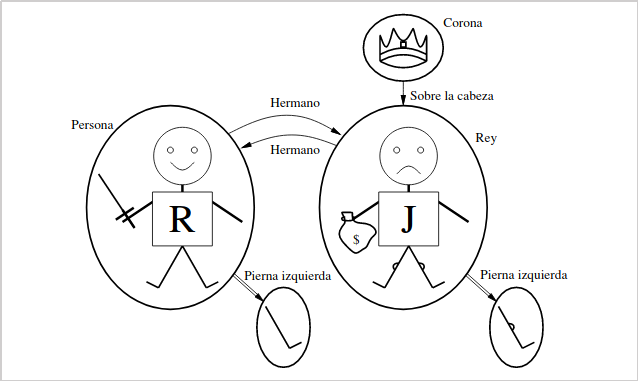
\includegraphics[width=14cm]{ia/Modelo-log-primer.png}
\caption{Modelo que contiene cinco objetos, dos relaciones binarias, tres relaciones unita-rias (indicadas mediante etiquetas sobre los objetos), y una función unitaria: pierna izquierda. Figura tomada de Russel Stuart; Norvig Peter. (2006). Inteligencia Artificial. Un enfoque moderno. Pearson Prentice Hall. Madrid, España.\cite{russell2004inteligencia} }

\label{fig:Modelo-log-primer} 
\end{figure}

En la figura \ref{fig:Modelo-log-primer} se puede observar un modelo en el que se incluye la noción de relaciones, funciones y objetos. A continuación, se describen los nuevos recursos de los que disponemos en la lógica de primer orden.

\begin{itemize}
\item \textbf{Objetos:} Nos permiten expresarnos acerca de los diferentes elementos en un determinado dominio. Al conjunto de todos los objetos utilizados se les conoce como \textbf{Dominio} o \textbf{Universo de discurso} \cite{guerra_repcon}.

\item \textbf{Función:} Una función es un tipo especial de relación que mapea un conjunto de objetos de entrada con un único objeto de salida. Al conjunto de todas las funciones se le conoce como \textbf{Base funcional} \cite{guerra_repcon}.

Las funciones nos sirven para evitar la necesidad de declarar muchos objetos, supongamos que tuviéramos como Dominio los estados de un país, si quisiéramos formar predicados que tuvieran como objetos sus capitales tendríamos dos opciones crear un nuevo objeto para cada estado o crear una función llamada por ejemplo: “capital”.

\item \textbf{Predicado:} El predicado indica relaciones entre objetos, al conjunto de todos los predicados se le conoce como \textbf{Base relacional} \cite{guerra_repcon}.

Supongamos que tenemos dos objetos, Juan y Pablo, si quisieramos indicar que Juan es hijo de Pablo podríamos hacerlo mediante el siguiente predicado:
esHijo(Juan,Pablo)

\item \textbf{Variables:} Son un elemento importante para la lógica de primer orden y suelen ser representadas mediante cualquier secuencia de caracteres que inicie con mayúscula, éstas variables representan a objetos del universo de discurso \cite{guerra_repcon}. 

Un ejemplo de un predicado que usa variables sería el siguiente: esHijo(X,Y), más adelante veremos cómo pueden usarse para expresar conocimiento.

\item \textbf{Cuantificadores:} El cuantificador universal $\forall$ que nos permite expresar relaciones acerca de todos los objetos en el dominio \cite{guerra_repcon}. \\

$\forall$ X podría leerse como “Para todo objeto X”.\\

El cuantificador existencial $\exists$ nos permite expresar la existencia de un objeto en el dominio \cite{guerra_repcon}. Por ejemplo podríamos expresar la siguiente oración: “Existe un objeto X que es azul y es grande”\\

$\exists$X esAzul(X) $\Lambda$ esGrande(X)\\

Se pueden utilizar múltiples cuantificadores en una fórmula pero es importante tomar en cuenta que el orden de lo mismo si importa, por ejemplo $\forall$X $\exists$Y es interpretado como para todo X existe un elemento Y, en cambio $\exists$X $\forall$Y es interpretado como existe algún elemento X para el cual todos los elementos Y.

\item \textbf{Términos:} Son todos los elementos que nos permitan denotar objetos y están formados por funciones, variables y constantes. Un ejemplo sería el siguiente calif ( hermano( alex ) , sma ) es un término que denota la calificación obtenida por el hermano de Álex en el curso de Sistemas Multi-Agentes \cite{guerra_repcon}.


\end{itemize}

Ahora veremos la sintaxis de la lógica de primer orden para posteriormente ver algunos ejemplos de fbf.

\begin{figure}[ht]
\centering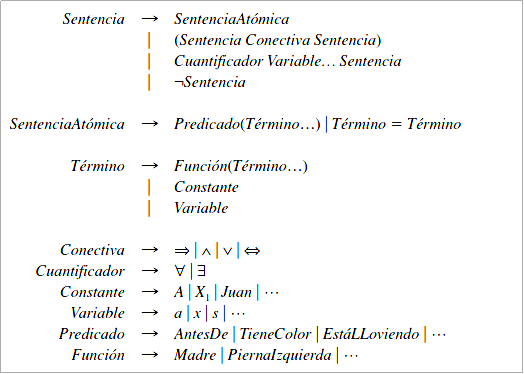
\includegraphics[width=14cm]{ia/sint-log-primer.png}
\caption{Sintaxis de la lógica de primer orden en BNF. Figura tomada de Russel Stuart; Norvig Peter. (2006). Inteligencia Artificial. Un enfoque moderno. Pearson Prentice Hall. Madrid, España. \cite{russell2004inteligencia} }

\label{fig:sint-log-primer} 
\end{figure}

\clearpage
Ahora veamos un ejemplo:

\underline{Dado como dominio las personas, representar el siguiente conocimiento:}

Todos los maestros son responsables\\
Algunos maestros son doctores\\
Todos los miembros del grupo son maestros o alumnos\\
Juan es maestro\\
Juan le da clase a Pedro\\
Algunos maestros le dan clase a todos los alumnos\\

\underline{Solución:}

D = { personas }\\
$\forall$X maestro(X) → responsable(X)\\
$\exists$X ( maestro(X) $\Lambda$ doctor(X) )\\
$\forall$X miembro(X) → ( maestro(X) v alumno(X) )\\
maestro(Juan)\\
daClase(Juan,Pedro)\\
$\exists$X $\forall$Y maestro(X) $\Lambda$ alumno(Y) $\Lambda$ daClase(X,Y)

\textbf{Sustitución en la lógica de primer orden}

La sustitución es un conjunto finito de pares de la forma \{ v1→t1, v2→t2, ... vn→tn \}, (también es utilizada la notación \{ v1/t1, v2/t2, ... vn/tn \}, cuando se aplica una sustitución a una expresión se obtiene una nueva, reemplazando en la expresión original cada aparición de la variable vi por el término ti (1 $\leq$ i $\leq$ n) \cite{navarro_prolog}.

Ejemplo:

$\alpha$ = esPequeño(x) $\Lambda$ juegaMucho(x) → esNiño(x)

Sust( {x/Juan}, $\alpha$ ) = esPequeño(Juan)  $\Lambda$ juegaMucho(Juan) → esNiño(Juan)

Sust( {x/hijo(Pedro)}, $\alpha$ ) 
= esPequeño(hijo(Pedro)) $\Lambda$ juegaMucho(hijo(Pedro)) → esNiño(hijo(Pedro))

\textbf{Inferencia en la lógica de primer orden}

\textbf{Reglas de inferencia para cuantificadores y proposicionalización}

Si eliminamos los cuantificadores de nuestros predicados podemos utilizar las reglas de inferencia de la lógica proposicional \cite{russell2004inteligencia}.

\underline{Regla de especificación universal:} Podemos inferir cualquier sentencia obtenida por sustitución de la variable por un término base (un término sin variables) \cite{russell2004inteligencia}.

\begingroup
\Large
\begin{equation}
\frac{\forall v  \; \alpha}{Sust(\{ v/g,\alpha \})}
\end{equation}
\endgroup

Ejemplo:

$\alpha$ = esPequeño(x) $\Lambda$ juegaMucho(x) → esNiño(x)

Sust( {x/Juan}, $\alpha$ ) = esPequeño(Juan)  $\Lambda$ juegaMucho(Juan) → esNiño(Juan)

\underline{Regla de especificación existencial:} Esta regla es más complicada ya que requiere que el símbolo de constante k no aparezca en ninguna otra parte de la base de conocimientos\footnote{ La base de conocimiento es el lugar donde se almacena el conocimiento del experto a manera de hechos y reglas, más adelante cuando se vea el tema de sistemas expertos se verá el rol de este elemento.} \cite{russell2004inteligencia}.

\begingroup
\Large
\begin{equation}
\frac{\exists v  \; \alpha}{Sust(\{ v/k,\alpha \})}
\end{equation}
\endgroup

Para reducir a la inferencia proposicional partimos de dos ideas \cite{russell2004inteligencia}:

\begin{itemize}
\item Toda sentencia que haga uso del cuantificador existencial se puede sustituir por el conjunto de todas las especificaciones posibles.
\item Mediante el uso de la regla de especificación universal, se pueden aplicar las sustituciones de todos los términos base posibles para obtener una base de conocimiento proposicional, a esta técnica se le conoce como proposicionalización.

\end{itemize}

Al hacer uso de estas ideas podemos aplicar posteriormente las reglas de inferencia vistas en el tema anterior.

\textbf{Modus Ponens Generalizado}

El Modus Ponens Generalizado es una versión del Modus Ponens que puede ser usada directamente en la lógica de predicados sin la necesidad de aplicar la proposicionalización.

La ventaja clave de este tipo de reglas “elevadas” es que solo realizan aquellas sustituciones que se necesitan para realizar la inferencia \cite{russell2004inteligencia}. A continuación se muestra el proceso de inferencia:

\begingroup
\Large
\begin{equation}
\frac{p_{1}^{'},p_{1}^{'},...,p_{n}^{'},(p_{1} \Lambda p_{2} \Lambda ... \Lambda p_{n} \rightarrow q)}{Sust(\theta,q)}
\end{equation}
\endgroup

Se tienen premisas de implicación $p_i$ y sentencias atómicas en nuestra base de conocimientos $p_{i}^{'}$, para aplicar esta regla de inferencia se tiene que encontrar una sustitución $\theta$ que permita que al aplicarse en las premisas de implicación y las sentencias de la base de conocimientos las haga idénticas.

A continuación se presenta un ejemplo:

\begin{tabular}{l}
	$\forall$x esPequeño(x) $\Lambda$ juegaMucho(x) → esNiño(x)\\
	esPequeño(Juan)\\
	juegaMucho(Juan)\\
\end{tabular}


\begin{tabular}{lll}
	$p_1$ = esPequeño(x) & $p_2$ = juegaMucho(x) & q = esNiño(x)\\
$p_{1}^{'}$ = esPequeño(Juan) & $p_{2}^{'}$ = juegaMucho(Juan) & 	\\

\end{tabular}

Para lograr que las sentencias atómicas sean iguales a las premisas de implicación se aplica la sustitución $\theta$ = \{ x/Juan \}, por lo tanto

Sust($\theta$,q) = esNiño(Juan)

\clearpage

Vamos a explorar un segundo ejemplo que contenga una sentencia atómica con una variable, para esto supondremos que todos los individuos de nuestro dominio juegan mucho:

\begin{tabular}{l}
	$\forall$x esPequeño(x) $\Lambda$ juegaMucho(x) → esNiño(x)\\
	esPequeño(Juan)\\
	$\forall$y juegaMucho(y)\\
\end{tabular}


\begin{tabular}{lll}
	$p_1$ = esPequeño(x) & $p_2$ = juegaMucho(x) & q = esNiño(x)\\
$p_{1}^{'}$ = esPequeño(Juan) & $p_{2}^{'}$ = juegaMucho(y) & 	\\

\end{tabular}

Para lograr que las sentencias atómicas sean iguales a las premisas de implicación se aplica la sustitución $\theta$ = \{ x/Juan \}, por lo tanto

Sust($\theta$,q) = esNiño(Juan)

\underline{Unificación}

Hasta este momento no nos hemos preguntado cómo encontrar el valor de la substitución que permita que expresiones lógicas distintas se hagan lógicas, a este proceso se le conoce como unificación \cite{russell2004inteligencia}.

Existen ocasiones donde se puede obtener más de un unificador, por ejemplo:

\begin{tabular}{l}
	Unificar( madre(María,x), madre(y,z) ) = \{ y/María, z/Juan, x/Juan \} \\
	Unificar( madre(María,x), madre(y,z) ) = \{ y/María, x/z \} \\
\end{tabular}


Si se realizan las sustituciones se puede observar que ambas unificaciones son válidas, generalmente se va a buscar obtener el \textbf{unificador más general (UMG)}, cada par de expresiones lógicas tiene su umg que es aquel que aplica menos restricciones sobre las variables. En el ejemplo anterior el umg sería: \{ y/María, x/z \}.

Existe un algoritmo para obtener el umg, sin embargo en este libro no se detallará su funcionamiento debido a que en las herramientas modernas no se suele tener la necesidad de programar el algoritmo de unificación.

Si se tienen dudas o se quiere profundizar en la lógica proposicional o de predicados recomiendo leer el libro de Russel y Norvig \cite{russell2004inteligencia}.

\subsection{Cláusulas de Horn} \index{Cláusulas de Horn}


Las cláusulas de Horn son fórmulas lógicas con una estructura particular, son una disyunción de literales con a lo sumo (como máximo) un literal positivo.

¬ $p_1$ v ¬ $p_2$ v ... ¬ $p_k$ v q

Una cláusula de Horn también puede ser representada de la siguiente forma (para lograr esta representación se hace uso de reglas de transformación, se hace uso de la ley de morgan y la regla de implicación material):

($p_1$ $\Lambda$ $p_2$ $\Lambda$ ... $\Lambda$ $p_k$) → q

A la literal no negada (q) se le conoce como la cabeza de la cláusula y al resto de literales se les conoce como el cuerpo.

\textbf{Importancia de las cláusulas de Horn}

Como veremos a lo largo de este tema, las cláusulas de Horn juegan un rol muy importante en la programación lógica, mediante el uso de este tipo de fórmulas lógicas se pueden utilizar mecanismos de inferencia eficientes.

\textbf{Desventajas de las cláusulas de Horn}

Si bien es cierto que limitan la expresividad de la lógica de primer orden generalmente son lo suficientemente expresivas para representar una vasta cantidad de conocimiento.

La inferencia con cláusulas de Horn es indecidible \footnote{ La indecidibilidad es la propiedad de un sistema de conducir siempre a una respuesta verdadera o falsa, por lo cual no siempre puede demostrar o refutar una sentencia.}. Sin embargo es semidecidible, cuando la fórmula es un teorema a veces se puede demostrar su validez, sin embargo cuando la fórmula no es un teorema siempre se puede demostrar su inconsistencia.

\textbf{Tipos de cláusulas de Horn}

A continuación se desglosan las tres posibles formas que puede tener una fórmula lógica y que cumplan con la estructura de una cláusula de Horn.
Las cláusulas determinadas son aquellas que tienen un literal positivo, estas a su vez se dividen en hechos y reglas, aquellas cláusulas que no tienen ningún literal positivo se llaman objetivos determinados.

\begin{tabular}{|l|l|}
\hline
	\thead{Nombre} & \thead{Estructura}\\
\hline
	Hecho & q\\
\hline
	Regla & ¬ $p_1$ v ¬ $p_2$ v ... ¬ $p_k$ v q\\
\hline
	Objetivo & ¬ $p_1$ v ¬ $p_2$ v ... ¬ $p_k$\\
\hline
\end{tabular}

\textbf{Inferencia mediante cláusulas de Horn}

\textbf{Encadenamiento hacia adelante}

Si tenemos nuestra base de conocimiento descrita mediante cláusulas de horn se puede realizar un algoritmo de encadenamiento hacia adelante muy sencillo que consiste en encontrar todas las reglas cuyo cuerpo pueda ser satisfecho con los hechos actuales y agregar a la base de hechos la cabeza de las reglas. Se repetirá el proceso hasta que no se puedan generar hechos nuevos o se haya comprobado algún objetivo. Hay que evitar añadir “renombramientos” a nuestra base de hechos, un renombramiento se da cuando sustituimos una variable por otra, lo cual da por resultado un predicado que tiene exactamente el mismo significado, ejemplo: 

Come(x, hamburguesa) significa lo mismo que Come(y, hamburguesa) 

En la figura \ref{fig:pse-enca-adel} se muestra el pseudocódigo del algoritmo de encadenamiento hacia adelante.

\begin{figure}[ht]
\centering\includegraphics[width=15cm]{ia/pse-enca-adel.png}
\caption{Algoritmo de encadenamiento hacia adelante simple. Figura tomada de Russel Stuart; Norvig Peter. (2006). Inteligencia Artificial. Un enfoque moderno. Pearson Prentice Hall. Madrid, España. \cite{russell2004inteligencia} }

\label{fig:pse-enca-adel} 
\end{figure}

Este algoritmo de encadenamiento es ineficiente ya que cada iteración trataría de agregar hechos ya conocidos, para mejorar la eficiencia se podría usar un encadenamiento hacia adelante incremental que utilizará solo aquellas reglas cuyo cuerpo contenga algún conjuntor $p_i$ que se unifique con un hecho obtenido en la iteración anterior. 

\FloatBarrier

\begin{center}
\line(1,0){420}
\end{center}

\textbf{Ejercicio de programación:}

Realizar un programa capaz de realizar encadenamiento hacia adelante usando cualquier lenguaje.Este ejercicio puede ayudar a comprender los conceptos aprendidos en este capítulo.

En mi caso usé (junto con mis compañeros de equipo en ese trabajo) el lenguaje de programación Java, añadiré el link al repositorio por si alguien quiere revisar el código del algoritmo.
\includegraphics[width=4cm]{Pictures/github/encad-adel.png}

(\url{https://github.com/amr205/LogicProgramming---Forward-chaining})

\textbf{Encadenamiento hacia atrás}

Con el encadenamiento hacia adelante vamos “descubriendo” nuevos hechos y paramos cuando no se pueden inferir nuevos hechos o se ha cumplido una meta. En el encadenamiento hacia atrás partimos de la meta que queremos demostrar y tratamos de determinar su validez.

Un algoritmo simple de encadenamiento hacia atrás sería el siguiente.
\begin{itemize}
\item Se tiene un objetivo
\item Se recorren las reglas y se selecciona la regla que permita unificar la cabeza de la regla con el objetivo, de esta manera se obtiene el umg y se sustituye el cuerpo de la regla con el umg, todos los predicados dentro de la regla se vuelven sub-objetivos y para cada uno de ellos se debe realizar este proceso.
\item Si no se encontró ninguna regla se recorren los hechos, si el objetivo es igual a algún hecho ese objetivo se considera como verdadero, en caso contrario se considera falso.
\end{itemize}

Veamos el siguiente ejemplo:

En nuestra base de conocimientos tenemos los siguientes hechos y reglas.

\begin{enumerate}
\item haceCroac(Fritz)
\item comeMoscas(Fritz)
\item haceCroac(x) $\Lambda$ comeMoscas(x)→esRana(x)
\item canta(x)$\Lambda$tieneAlas(x)→esCanario(x)
\item esRana(x)→esVerde(x)
\item esCanario(x)→esAmarillo(x)
\end{enumerate}

El objetivo es determinar si: esVerde(Fritz)

A continuación se muestra un diagrama de cómo se realiza el encadenamiento hacia atrás para demostrar que el objetivo es verdadero.

\begin{figure}[ht]
\centering\includegraphics[width=12cm]{ia/BC-esRana.png}
\caption{Proceso de encadenamiento hacia atrás del objetivo esVerde(Fritz).}

\label{fig:BC-esRana} 
\end{figure}

\textbf{Mecanismo de resolución SLD}

Para realizar un encadenamiento hacia atrás podemos utilizar el mecanismo de resolución SLD (Selective Linear Definite clause resolution). Para explicar cómo funciona este mecanismo primero hay que entender la función de selección $\varphi $, esta función dado un objetivo Q devuelve uno y solo uno de los átomos de Q.

\clearpage
Ejemplo:
 
Q = $A_1$ $\Lambda$ $A_2$ $\Lambda$ $A_j$ $\Lambda$...$\Lambda$ $A_n$\\
$\varphi $(Q) = $A_j$

\textbf{Funcionamiento del mecanismo de resolución SLD}

En este caso la función de selección devolverá el primer átomo del objetivo.
Dado un objetivo Q de la forma $A_1$ $\Lambda$ $A_2$ $\Lambda$ $A_j$ $\Lambda$...$\Lambda$ $A_n$. se buscará la primera sentencia C del programa $B_1$ $\Lambda$ ... $\Lambda$ $B_m$ → H tal que $\varphi $(Q) = A y H sean unificables por un umg $\theta$. Entonces la nueva pregunta $Q^{'}$ (el resolvente) será igual a la sustitución Sust( ($B_1$ $\Lambda$ ... $\Lambda$ $B_m$ $\Lambda$ $A_2$ $\Lambda$ ... $\Lambda$ $A_n$), $\theta$). El proceso continuará de igual forma hasta obtener la pregunta vacía (lo que corresponde a un éxito, se obtiene una pregunta vacía si existe un umg $\theta$ tal que Sust(Q,$\theta$)=Sust(C,$\theta$)), o una pregunta para la cual no exista resolvente con ninguna sentencia del programa (lo que corresponderá a un fracaso) \cite{navarro_prolog}.

Vamos a explorar este proceso separándolo en pasos:

\begin{enumerate}
\item Se tiene un objetivo Q de la forma $A_1$ $\Lambda$ $A_2$ $\Lambda$ $A_j$ $\Lambda$...$\Lambda$ $A_n$
\item Se selecciona un átomo A del objetivo Q, A = $\varphi $(Q)
\item Se busca la primera sentencia C de la forma $B_1$ $\Lambda$ ... $\Lambda$ $B_m$ → H tal que A y H sean unificables por un umg $\theta$. 
\item Se obtiene el nuevo resolvente (también llamado derivación ya que $Q^{'}$ deriva de Q),  $Q^{'}$ = Sust( ($B_1$ $\Lambda$ ... $\Lambda$ $B_m$ $\Lambda$ $A_2$ $\Lambda$ ... $\Lambda$ $A_n$), $\theta$)
En este paso cuando la sentencia C es un hecho solo se tendría la cabeza H de la cláusula por lo cual $Q^{'}$ sería igual a $Q^{'}$ = Sust( ($A_2$ $\Lambda$ ... $\Lambda$ $A_n$), $\theta$)
\end{enumerate}

Este proceso se repite siendo $Q^{'}$ el nuevo objetivo hasta que se cumpla una de las siguientes condiciones:
\begin{itemize}
\item En el paso 3 no se encontró ninguna sentencia que permita generar un nuevo resolvente, por lo cual la resolución fracaso.
\item Tras el paso 4 $Q^{'}$ es igual a una pregunta vacía, lo que corresponde a un éxito.
\end{itemize}

\subsection{Sistemas expertos} \index{Sistemas expertos}

Los sistemas expertos son sistemas basados en conocimiento diseñados para realizar tareas que normalmente requerirán un experto. Estos sistemas son usados para resolver problemas de dominio específico y se comportan como un sistema asesor en la toma de decisiones \cite{tms_ES}.

El desarrollo de los sistemas expertos empezó alrededor del año 1965 con un proyecto de Edward Feigenbaum, a quien se le atribuye el título de padre de los sistemas expertos), el desarrollo de estos sistemas continuó durante las siguientes décadas, donde fueron utilizados tanto en la industria como académicamente. Su auge fue durante el boom de la inteligencia artificial (1980–1987), en la actualidad la popularidad de los sistemas expertos ha decaído y si bien existen sistemas expertos implementados en diversas aplicaciones la opinión popular parece indicar que fallaron en cumplir las expectativas esperadas \cite{leph_ES}.

\textbf{Componentes de los sistemas expertos}

A continuación se describen los principales componentes de un sistema experto \cite{tms_ES}:
\begin{itemize}
\item \underline{Interfaz de usuario:} Es el mecanismo mediante el cual el usuario final va a interactuar con el sistema experto.
\item \underline{Base de conocimiento:} Contiene todo el conocimiento adquirido del experto a manera de reglas y hechos.
\item \underline{Motor de inferencia:} Es el mecanismo que se encarga de realizar la inferencia manipulando las reglas y hechos de la base de conocimiento.
\item \underline{Subsistema de explicación o justificación:} Este módulo o subsistema es el encargado de explicar el razonamiento mediante el cual el sistema experto llegó a una conclusión.
\item \underline{Subsistema de adquisición de conocimiento:} Este módulo o subsistema permite al usuario añadir nuevo conocimiento sin la necesidad de que un ingeniero o personal especializado se vea involucrado en este proceso.
Algunos sistemas expertos cuentan con un módulo de aprendizaje que les permite adaptarse de acuerdo a la información que reciben.
\end{itemize}

\begin{figure}[ht]
\centering\includegraphics[width=12cm]{ia/SistemaExperto.png}
\caption{Representación gráfica de los componentes de un sistema experto.}

\label{fig:SistemaExperto} 
\end{figure}

\textbf{Desarrollo de un sistema experto}

Para el desarrollo de un sistema experto se tiene que realizar la extracción del conocimiento para posteriormente desarrollar el sistema. A continuación se presentan algunos pasos sugeridos que se pueden seguir durante el desarrollo:

\begin{enumerate}
\item \underline{Identificación del problema:} Es muy importante saber qué problema pretende resolver nuestro sistema experto y los objetivos que van a utilizar nuestros usuarios finales. También en esta fase el desarrollador debe realizar una investigación sobre el dominio del problema con el fin de tratar de adquirir conocimiento general sobre el problema o situación a resolver. Posteriormente se debe obtener información de expertos mediante técnicas como la entrevista (es importante la investigación previa para realizar preguntas puntuales).
\item \underline{Conceptualización del conocimiento:} En esta fase se debe representar el conocimiento mediante técnicas como los marcos, redes semánticas, etc. Existen libros sobre la ingeniería del conocimiento que repasan este tipo de técnicas. En esta sección se recomienda mantener la comunicación con el experto para que nos indique si nuestras representaciones son adecuadas y coinciden con su conocimiento.
\item \underline{Formalización del conocimiento:} El conocimiento se va a representar mediante un modelo formal, es importante tomar en cuenta como va a funcionar nuestro modelo de inferencia, lo más probable es que tengamos que representar nuestro conocimiento mediante el uso de cláusulas de Horn.
\item \underline{Implementación del sistema experto:} En esta fase se desarrollará el sistema experto y se realizará la programación necesaria, se pueden usar herramientas existentes para facilitar el desarrollo.
\item \underline{Validación y mantenimiento del sistema:} Se debe validar que las respuestas del sistema experto y de los expertos coincidan de manera consistente.
\end{enumerate}

\textbf{Uso del lenguaje de programación prolog}

PROLOG es un lenguaje declarativo de programación lógica diseñado para representar y utilizar el conocimiento que se tiene sobre un determinado dominio.

\textbf{¿Qué es un lenguaje declarativo?}

Existen dos estilos principales en los lenguajes de programación, imperativos y declarativos. Los programas en los lenguajes imperativos constan de instrucciones que nos permiten modificar el estado de un programa mediante la modificación de variables, básicamente se describe el proceso de cómo hacer algo; ejemplos de estos lenguajes son Java, C++, PHP. En los programas de los lenguajes declarativos se describe qué se quiere hacer pero no se especifica el cómo; PROLOG es un ejemplo de este tipo de lenguajes.

\textbf{Sintaxis de la base de conocimientos}

En un programa de prolog se pueden guardar reglas y hechos, estas reglas y hechos deben ser cláusulas de Horn, a continuación se describe la sintaxis:
Los objetos tienen que iniciar con minúscula y las variables con mayúscula.

\underline{Sintaxis de una regla en prolog}

Cabeza :- Cuerpo.

Las cláusulas del cuerpo pueden estás separadas por “,” que representa una conjunción o “;” que representa una disyunción.

Ejemplo:

haceCroac(x)$\Lambda$comeMoscas(x)→esRana(x)

Esta regla se representaría de la siguiente manera en prolog:

esRana(X) :- haceCroac(X),comeMoscas(X).

\underline{Sintaxis de un hecho en prolog}

Cabeza.

Ejemplo:

haceCroac(Fritz)

Este hecho se representaría de la siguiente manera en prolog:

haceCroac(fritz).

\textbf{Objetivos en prolog}

Una vez tenemos descrita nuestra base de conocimientos podemos realizar “preguntas” mediante los objetivos. Para preguntar ¿es fritz verde? construiríamos el objetivo en prolog “esVerde(fritz).”, también podemos hacer uso de variables para preguntar ¿Quién es verde? construyendo el objetivo de la siguiente manera “esVerde(X).”.

\textbf{Inferencia en prolog}

Prolog utiliza como método de inferencia el mecanismo de resolución SLD descrito anteriormente en este libro.

\clearpage

\textbf{Ejercicio de programación:}

Realizar el desarrollo de un sistema experto del tema que el lector prefiera y usando cualquier lenguaje de programación. Yo recomiendo utilizar un lenguaje de programación como prolog para no tener que realizar la programación del motor de inferencia.

\includegraphics[width=5cm]{Pictures/github/sisema-experto.png}

(\url{https://github.com/amr205/animals-prolog})

\part{Parte cuatro: Machine Learning}

\chapterimage{chapter_head.pdf} % Chapter heading image

\chapter{Introducción al capítulo}

\section{Definición} \index{Definición}

El machine learning o aprendizaje automático es una disciplina del campo de la inteligencia artificial que pretende generar sistemas capaces de aprender a través de la “experiencia”.
El problema de aprendizaje puede ser descrito de la siguiente manera: 
Un programa se dice que aprende a través de la experiencia $E$ con respecto a un tipo de tareas $T$ y una medición de su desempeño $P$, si su desempeño en las tareas $T$, medidas por $P$, mejora a través de la experiencia E \cite{mitchell1997machine}.

Esta definición puede ser muy formal sin embargo describe un problema general sobre el cual se puede aplicar machine learning. Dicho de forma más simple en el aprendizaje automático no se desarrolla de manera explicita la lógica que nos permite ir de unos datos de entrada a un resultado, en cambio se proporcionan datos de entrada junto con los resultados que esperamos aprender y los usamos para entrenar un algoritmo de aprendizaje, este algoritmo genera un "programa" que nos permite predecir el resultado a partir de nuevos datos de entrada.

\begin{figure}[ht]
\centering\includegraphics[width=12cm]{ia/whatisml.png}
\caption{Comparación entre la programación tradicional y el aprendizaje automático.}

\label{fig:whatisml} 
\end{figure}

\FloatBarrier

\section{Clasificación} \index{Clasificación}

Existen tres tipos de algoritmos principales dependiendo del tipo de aprendizaje que realizan, a continuación se describen de manera breve:
\begin{itemize}
\item \textbf{Aprendizaje supervisado:} Se aprende a través de ejemplos que se encuentran previamente clasificados o emparejados con un valor, un ejemplo puede ser un clasificador de imágenes que debe aprender a distinguir entre perros y gatos que para el proceso de aprendizaje requerirá de un conjunto de imágenes asociadas a la clase correcta.
\item \textbf{Aprendizaje no supervisado:} Este tipo de algoritmos aprenden a través de ejemplos sin clasificar y tienen que aprender patrones que les permitan organizarlos de alguna manera, un ejemplo podría el siguiente: una tienda de ropa necesita elegir las medidas que tendrán sus prendas de ropa para las tallas chica, mediana y grande, con el objetivo de lograr esto se recopilan las medidas de la gente que vive cerca de la tienda y se utiliza un algoritmo de machine learning que le indica cuales serían las medidas adecuadas (más adelante en este libro veremos que clase de algoritmo podría ser útil para esta tarea).
\item \textbf{Aprendizaje semi-supervisado:} En este tipo de algoritmo nuestro set de entrenamiento contiene ejemplos clasificados y no clasificados, la mayoría de los ejemplos no suelen estar clasificados, aunque usar ejemplos sin clasificar pueda parecer contra-intuitivo estos añaden información sobre el problema lo que puede resultar en un mejor modelo.
\item \textbf{Aprendizaje reforzado:} Este tipo de algoritmos aprenden a través de la experiencia, interactúan con su entorno y reciben recompensas que les indican si las acciones realizadas han sido correctas o no.
\end{itemize}

\section{Problemas que resuelve} \index{Problemas que resuelve}

Los algoritmos de machine learning nos permiten resolver principalmente problemas de clasificación,regresión, asociación y agrupamiento, a continuación se describe su significado \cite{burkov2019hundred}:

\begin{itemize}
\item \textbf{Clasificación:} este problema consiste en asignar una etiqueta a un ejemplo sin clasificar, uno de los ejemplos más famosos es la detección de spam.
\item \textbf{Regresión:} este problema consiste en predecir un valor dado un ejemplo sin etiquetar, por ejemplo otorgar las características de una casa y predecir su costo.
\item \textbf{Agrupación (Clustering):} Consiste en agrupar los datos de tal forma que los elementos de estos grupos sean similares, esto puede ser útil por ejemplo para segmentar nuestros clientes según su forma de comprar.
\item \textbf{Asociación:} Consiste en relacionar instancias de nuestro set de entrenamiento con características similares, por ejemplo encontrar la noticia más similar a la que acaba de leer el usuario.
\end{itemize}

\begin{figure}[ht]
\centering\includegraphics[width=14cm]{ia/mltasks.png}
\caption{Clasificación del aprendizaje automático y los tipos de problemas o tareas que pueden solucionar.}

\label{fig:mltasks} 
\end{figure}

\textbf{¿En este libro ya utilizamos machine learning?}

Si, en el tema Sistemas clasificadores (Learning classifier system) realizamos algoritmos de machine learning y precisamente vimos como uno de ellos pertenece a la categoría de aprendizaje supervisado y el otro a la categoría de aprendizaje reforzado.

\section{Importancia del machine learning} \index{Importancia del machine learning}

Este tipo de algoritmos nos permiten resolver tareas que de otra manera serían prácticamente imposibles, por poner un ejemplo simple, sin el uso de este tipo de algoritmos cómo sería posible crear un algoritmo al cual le dieras una imagen y la clasificara como un perro o un gato.

Hoy en día el machine learning ha sido aplicado en una variedad de ámbitos de manera exitosa, a continuación se listan algunos de ellos:

\begin{itemize}
\item Procesamiento del lenguaje natural
\item Computer vision (Procesamiento de imágenes)
\item Evaluación de clientes
\item Sistemas de recomendación
\item Sistemas de detección de anomalías
\item Reconocimiento de genes en secuencias de ADN
\item Etc.
\end{itemize}

El paradigma simbólico visto en el capítulo anterior tiene el problema de que el aprendizaje no se adquiere directamente del entorno o a través de ejemplos, por lo cual hay dominios muy complejos de modelar o al ser vaciado el conocimiento se corre el riesgo de perder detalles importantes del modelo, el machine learning hoy en día presenta una gran oportunidad debido a que la cantidad de datos e información generada en estos últimos años hacen posible el uso de estos algoritmos para la resolución de problemas complejos.

\chapterimage{chapter_head.pdf} % Chapter heading image

\chapter{Aprendizaje supervisado}

\section{Introducción al capítulo} \index{Introducción al capítulo}

En este capítulo se revisarán diversos algoritmos de machine learning que utilizan aprendizaje supervisado, antes de revisar distintos algoritmos que realizan la tarea de clasificación o regresión vamos a observar algunas generalidades presentes en este tipo de aprendizaje.

El proceso suele iniciar con la recolección de los datos. Estos datos van a conformar nuestro conjunto de datos (dataset), consisten de una serie de pares de datos (entrada, salida). Los valores de entrada pueden ser cualquier cosa, correos, imágenes, etc. Los valores de salida pueden ser etiquetas que correspondan a una clase (perros, gatos, etc), valores numéricos (precio, probabilidad, etc), o secuencia de datos \cite{burkov2019hundred}.

Para poder procesar los datos la entrada suele estar compuesta de un vector de atributos (feature vector ó attribute vector), por ejemplo si cada elemento de nuestro conjunto de datos esta compuesto de color, anchura y altura, nuestro vector de atributos debería representar adecuadamente esto, algunos algoritmos requieren que nuestros vectores estén compuestos de datos númericos, por lo cual para el ejemplo anterior se podría descomponer el atributo de colos en tres atributos que serían el valor de la intensidad del color en el canal rojo, azul y verde. El vector de atributos de una instancia con color azul, anchura de 3 metros y altura de 15 sería el siguiente: [ 0,0,1,3,15 ], al número de atributos de nuestro vector se le conoce como dimensionalidad, en este ejemplo simple se tiene una dimensionalidad de 6.

Es deber del analista de datos determinar cómo convertir una entidad del mundo real a un vector de atributos y como transformar o extraer las características relevantes del problema. Un ejemplo más complejo sería el convertir un correo electrónico, esta tarea la dejaré para más adelante ya que será uno de los ejercicios a realizar en temas posteriores.

Los tipos de atributos que puede contener nuestro conjunto de datos son los siguientes:
\begin{itemize}
\item \textbf{Datos numéricos:} Estos tipo de datos pueden ser números continuos (Que pueden tomar cualquier valor dentro de un rango) o discretos (Solo pueden tomar ciertos valores dentro de un rango), los datos numéricos continuos suelen ser usados en medidas como la altura, el peso, etc y los datos numéricos discretos en aquellas cosas que deben ser contabilizadas como el número de hijos, número de ocurrencias de un evento, etc.
\item \textbf{Datos ordinales:} Son aquellos datos en los que existen variables en categorías ordenadas, la distancia entre dos categorías no se establece en este tipo de datos, por ejemplo si tuviéramos el atributo ``calidad del servicio'' este campo podría tomar los siguientes valores \{  ``malo'', ``regular'', ``bueno'', ``excelente'' \} y se da por entendido que el valor ``malo'' es más cercano a ``regular'' que a ``excelente''.
\item \textbf{Datos categóricos:} Son aquellos datos en los que existen variables en categorías no ordenadas, por ejemplo el color de un auto \{ ``rojo'', ``azul'', ``amarillo'', ``verde''\}.
\end{itemize}

En el aprendizaje automático también se suelen usar como datos el texto que suele estar compuesto de una serie de palabras, o las secuencias temporales que contienen datos asociados a un valor temporal como fecha, hora o fecha y hora.

Nuestro conjunto de datos suele estar dividido en otros subconjuntos, al inicio de este capítulo usaremos solamente el set de entrenamiento pero más adelante veremos cómo utilizar los otros, a continuación se describen los principales subconjuntos:


\begin{itemize}
\item \textbf{Set de entrenamiento (training set):} Estos elementos que ya poseen clasificación son aquellos que nos servirán para entrenar a nuestro algoritmo.
\item \textbf{Set de prueba (test set):} Con estos elementos se probará el desempeño de nuestro algoritmo, usando instancias que nuestro algoritmo no observó durante el entrenamiento.
\item \textbf{Set de validación (validation set):} Este conjunto se utiliza para ajustar parámetros del algoritmo para obtener un mejor resultado, dependiendo del algoritmo existen diferentes hiperparametros \footnote{ Un hiperparámetro es una propiedad del algoritmo de aprendizaje, estos valores no son aprendidos a partir del proceso de aprendizaje y tienen que ser determinados por el desarrollador.} a optimizar y también existen diferentes técnicas para usar este conjunto.
\end{itemize}

Usando nuestro conjunto de datos, aplicaremos un \textbf{algoritmo de aprendizaje}, existen dos divisiones principales de estos algoritmos:

\begin{itemize}
\item \textbf{Algoritmos de aprendizaje paramétricos:} Estos algoritmos optimizan una función de una forma determinada, por ende hacen suposiciones acerca de la forma de la función de la cual provienen los datos, para optimizar esta función se aprenden los valores de los parámetros a través del proceso de aprendizaje. Ejemplos de parámetros son los pesos en las redes neuronales, los coeficientes en regresión lineal o los vectores de soporte en una máquina de soporte de vectores.
\item \textbf{Algoritmos de aprendizaje no paramétricos:} Estos algoritmos no hacen suposiciones acerca de la forma que tiene la función de la cual provienen los datos, por lo cual carecen de parámetros que se estiman a partir de los datos de entrada. 
\end{itemize}

Los algoritmos de aprendizaje no paramétricos tienen la ventaja de que al no hacer suposiciones sobre la forma de la función es posible obtener muy buenos modelos, sin embargo tienen la desventaja de tener un proceso de aprendizaje y predicción generalmente mayor en comparación a los algoritmos de aprendizaje paramétricos, además de usualmente requerir mayor cantidad de datos de entrenamiento para dar buenos resultados.

Los algoritmos de aprendizaje paramétricos suelen estar compuestos de lo siguiente \cite{burkov2019hundred}:

\begin{itemize}
\item \textbf{Una función de pérdida (loss function):} Nos permite medir la diferencia entre el resultado obtenido por el algoritmo de aprendizaje y el valor de salida real de una sola instancia.
\item \textbf{Un criterio de optimización (optimization criteria):} El criterio mediante el cual se va medir la efectividad del modelo, este criterio está basado en la función de pérdida, un ejemplo podría ser \textbf{una función de coste o error (cost function)}, esta función mide el error del algoritmo de aprendizaje a través de todas las instancias, suele ser el promedio del valor obtenido al aplicar la función de pérdida sobre cada instancia.
\item \textbf{Una rutina de optimización (optimization routine):} Este es el proceso mediante el cual se va a manejar la información para encontrar una solución al criterio de optimización.
\end{itemize}

El resultado de aplicar el algoritmo de aprendizaje sobre un conjunto de datos es un \textbf{modelo}, este modelo nos permitirá realizar predicciones sobre los nuevos elementos no asociados a una información de salida.

En la especialización de machine learning realizado por la Universidad de Washington en la plataforma de Coursera se presenta una imagen similar a la siguiente que muestra los elementos descritos anteriormente.

\begin{figure}[ht]
\centering\includegraphics[width=14cm]{ia/Aprendizaje supervisado diagrama.png}
\caption{Diagrama representando un problema de aprendizaje supervisado, donde se tiene un set de entrenamiento con datos de entrada X y datos de salida Y, se entrena un modelo con parámetros W para generar predicciones Ŷ}

\label{fig:Aprendizaje-supervisado-diagrama} 
\end{figure}
\FloatBarrier

Se invita al lector a identificar los elementos aquí descritos en el tema UCS (LCS con aprendizaje supervisado) de este libro.

Antes de explorar algunos de los diferentes algoritmos de aprendizaje vamos a revisar una rutina de optimización que nos permitirá aprender los parametros $W$ de nuestros modelos. Es por esto que se motiva al lector entender claramente las partes y procesos que forman parte del aprendizaje supervisado presente en la figura \ref{fig:Aprendizaje-supervisado-diagrama}.

\clearpage

\section{Descenso del gradiente} \index{Descenso del gradiente}

En esta sección examinaremos el funcionamiento básico de la rutina de optimización llamada descenso del gradiente, esta rutina tiene diversas variantes y algunas implementaciones más complejas que pretenden mejorarla sin embargo en este capitulo nos centraremos en la más simple.

\textbf{¿Porqué este tema se encuentra en esta sección del libro?}

Al inicio puede parecer un poco contra intuitivo el revisar este tema antes de ver algún algoritmo de aprendizaje de regresión o clasificación, sin embargo esta rutina es utilizada por diversos algoritmos y es ampliamente usada actualmente, por lo cuál considero importante que el lector entienda su funcionamiento de manera general para posteriormente ver su implementación específica en los temas posteriores. Otra razón para colocar esta información aquí es la posibilidad de encontrarlo fácilmente en el índice por si se requiere repasar el funcionamiento de esta rutina de optimización.

\textbf{¿Qué es el descenso del gradiente?}

El descenso del gradiente es una manera de minimizar una función objetivo (referido como criterio de optimización en la introducción del capítulo) J($\theta$) donde los parámetros del modelo $\theta \in \mathbb{R}^{d}$ son ajustados de manera iterativa en la dirección contraria al gradiente de la función objetivo respecto a los parámetros $\nabla _{\theta} J(\theta)$ \cite{ruder2017overview}.

Esta definición formal es bastante adecuada una vez se entienden los conceptos que se están utilizando, sin embargo puede carecer de sentido antes de entender lo que esta realizando conceptualmente, por ello a continuación vamos a revisar los diferentes elementos descritos.

\underline{Función objetivo $J(\theta)$}

La función objetivo como fue descrito en la introducción del capítulo mide la efectividad de nuestro modelo usando generalmente una función de coste o error, mientras menor sea el valor quiere decir que el desempeño de nuestro algoritmo de aprendizaje es mejor. Por intuición sabemos que hay una combinación de valores en nuestros parámetros $\theta$ que minimizan esta función objetivo.

Para simplificar el problema y para poder mostrar de manera gráfica esta situación en la figura \ref{fig:cost_function_min} se puede observar que existe un valor para $\theta_1$ que minimiza la función $J(\theta)$.


\begin{figure}[ht]
\centering\includegraphics[width=6cm]{ia/cost_function_min.png}
\caption{Representación visual de la función $J(\theta)$, en esta figura el valor mínimo de $J(\theta)$ se encuentra señalado con un punto rojo}

\label{fig:cost_function_min} 
\end{figure}

\underline{Gradiente $\nabla _{\theta} J(\theta)$}

Cuando nosotros empezamos el entrenamiento iniciamos con valores aleatorios de $\theta$ por lo cual nuestro objetivo es lograr encontrar los valores $\theta$ que optimizen la función  $J(\theta)$, entonces nuestra pregunta es ¿Cómo pasar de nuestro valor inicial al valor óptimo?.

\begin{figure}[ht]
\centering\includegraphics[width=9cm]{ia/cost_function_min_init.png}
\caption{Representación visual de la función $J(\theta)$, en esta figura el valor mínimo de $J(\theta)$ se encuentra señalado con un punto rojo y el valor inicial se encuentra marcado con el punto verde}

\label{fig:cost_function_min_init} 
\end{figure}

En el caso presentado en la figura \ref{fig:cost_function_min_init} solo tenemos un parámetro $\theta$ por lo cual mediante el uso de una derivada podemos obtener la pendiente e ir en la dirección contraria para irnos acercando al valor de $\theta$ que minimize $J(\theta)$.

Recordemos que podemos entender una derivada $dy/dx$ de una función $y=f(x)$ como una razón de cambio respecto a la variable x (visualizada como una tangente en el punto que se deriva, o la pendiente de la función en un punto determinado), entonces de esta manera al calcular la derivada de $J(\theta)$ respecto a $\theta$ podemos obtener la dirección hacia la cual debemos llevar nuestro valor $\theta$ para minimizar la función.

\begin{figure}[ht]
\centering\includegraphics[width=7cm]{ia/cost_function_der.png}
\caption{Representación visual de la función $J(\theta)$, en esta figura el valor mínimo de $J(\theta)$ se encuentra señalado con un punto rojo y el valor inicial se encuentra marcado con el punto verde y la recta tangente a la función $J(\theta)$ se encuentra dibujada con color negro.}

\label{fig:cost_function_der} 
\end{figure}

¿Qué hacemos si tenemos más de un parámetro?

La respuesta es relativamente sencilla, el objetivo es obtener el gradiente, el gradiente es una generalización multivariable de la derivada. Mientras que una derivada se puede definir solo en funciones de una sola variable, para funciones de varias variables, el gradiente toma su lugar. El gradiente es una función de valor vectorial, a diferencia de una derivada, que es una función de valor escalar.  De esta manera al obtener el gradiente sabremos en que dirección actualizar cada uno de nuestros parámetros.

El cálculo del gradiente dependerá del algoritmo de aprendizaje que se este utilizando por lo cual en este momento no veremos ningún ejemplo en específico.

\underline{Descenso del gradiente}

Ahora que sabemos que es el gradiente y porqué queremos obtenerlo, el descenso del gradiente tiene mucho más sentido.

Esta rutina de optimización en su forma más básica (Descenso del gradiente por lotes o Batch Gradient Descent) consiste en calcular el gradiente de la función objetivo $J(\theta)$ respecto a los parámetros $\theta$ a través de todo el set de entrenamiento para de manera iterativa ajustar los parámetros del algoritmo de aprendizaje de acuerdo a la siguiente fórmula:

\begin{equation}
\label{eqn:gradient_descent}
\theta = \theta - \alpha \cdot  \nabla _{\theta} J(\theta)
\end{equation}

Donde: 

\begin{tabular}{l}
\makecell[l]{$\alpha$ es un parámetro de la rutina de optimización llamado tasa de aprendizaje (learning rate) que \\ controla que tan grande es la actualización de los parámetros.} \\
\makecell[l]{$\theta$ es el vector de parametros.} \\
\makecell[l]{$\nabla _{\theta} J(\theta)$ es el gradiente de la función de costo respecto a los parámetros.} \\
\end{tabular}

Es importante no usar valores muy grandes de $\alpha$ ya que podríamos no llegar a ningún mínimo local, sin embargo valores muy bajos de $\alpha$ harán que tardemos mucho en llegar al mínimo. Más adelante dentro del tema de machine learning se verán algunas técnicas para ajustar los parámetros de nuestros algoritmos de aprendizaje. Para finalizar este tema me gustaría mostrar la siguiente imagen sacada del curso de Machine Learning en Coursera impartido por Andrew Ng.

\begin{figure}[ht]
\centering\includegraphics[width=9cm]{ia/gd_andrewng.png}
\caption{Descenso del gradiente con dos parámetros $\theta_0$ y $\theta_1$}

\label{fig:cost_function_der_two_params} 
\end{figure}

\textbf{Variaciones del descenso del gradiente}

A continuación se listan distintas variaciones de esta rutina de optimización para que al momento de estar aplicando este tipo de algoritmos en la vida real cuando el lector se encuentre con dichas variaciones tenga un lugar para consultar sus diferencias, así como revisar sus ventajas y desventajas. Si es tu primera vez leyendo este libro recomiendo continuar con la siguiente sección y volver al terminar el cápitulo.

\begin{itemize}

\item \textbf{Batch gradient descent}: Versión básica de esta rutina de optimización, se utilizan todos los elementos del conjunto de datos para calcular el gradiente.
\begin{equation}
\label{eqn:batch_gradient_descent}
\theta = \theta - \alpha \cdot  \nabla _{\theta} J(\theta)
\end{equation}

\item \textbf{Stochastic Gradient Descent (SGD):}: En esta variante del descenso del gradiente se actualiza el valor de los parametros calculando el gradiente para cada uno de los elementos en el conjunto de datos.
\begin{equation}
\label{eqn:stochastic_gradient_descent}
\theta = \theta - \alpha \cdot  \nabla _{\theta} J_{i}(\theta)
\end{equation}
Donde:

\begin{tabular}{l}
\makecell[l]{$\nabla _{\theta} J_{i}(\theta)$ es el gradiente de la función de costo respecto a los parámetros en un solo \\elemento del conjunto de datos seleccionado al azar.} \\
\end{tabular}

\underline{Ventajas:}
Ayuda a lograr una convergencia más rápida cuando el conjunto de datos es muy grande.

\underline{Desventajas:}
Debido a las altas variaciones en cada actualización de valores en los parámetros es posible que no converja en un optimo global .
\\

\item \textbf{Mini-batch Gradient Descent:}: En esta variante del descenso del gradiente se actualiza el valor de los parametros calculando el gradiente en un subconjunto aleatorio de tamaño m del conjunto de datos.
\begin{equation}
\label{eqn:mini_batch_gradient_descent}
\theta = \theta - \alpha \cdot   \frac{1}{m} \sum_{i=1}^{n}  \nabla _{\theta} J_{i}(\theta)
\end{equation}
\underline{Ventajas:}
Otorga un balance entre costo computacional y velocidad, puede ser utilizado en conjuntos de datos grandes.

\underline{Desventajas:}
Es necesario elegir el valor de $m$ para el subconjunto de datos.
\\

\item \textbf{Momentum Gradient Descent:}: En esta variante se añade ``momento'' a la actualización de los parámetros.
\begin{equation}
\label{eqn:momentum_gradient_descent}
\begin{split}
v_{t} &= \gamma v_{t-1} + \alpha \cdot  \nabla _{\theta} J(\theta_{t-1})
\\
\theta_{t} &= \theta_{t-1} - v_{t+2}
\end{split}
\end{equation}
Donde:

\begin{tabular}{l}
\makecell[l]{$v_{t}$ es el vector de velocidad en la iteración $t$.} \\
\makecell[l]{$\gamma$ es el coeficiente de momento, este hiperparámetro controla la contribución del \\
vector de velocidad anterior.} \\
\end{tabular}

\underline{Ventajas:}
En funciones con mucho ruido o curvatura ayuda a evitar que se converja en un óptimo local.

\underline{Desventajas:}
Si el valor de $\gamma$ es grande el vector de parámetros puede oscilar alrededor del valor óptimo (local o global).
\\

\item \textbf{Adagrad}: En esta variante el valor de la tasa de aprendizaja se adapta para cada parametro basado en el valor historico del gradiente. Parametros con un valor grande en el gradiente tienen una tasa de aprendizaje reducida, aquellos con un valor pequeño en el gradiente tienen una tasa de aprendizaje aumentada.

\underline{Ventajas:}
En funciones con parametros en diferentes escalas ayuda a acelerar la convergencia en un valor optimo.

\underline{Desventajas:}
Debido a que reduce la tasa de aprendizaje con valores grandes en el historico del gradiente, el aprendizaje puede llegar a detenerse antes antes de converger en un óptimo
\\

\item \textbf{RMSProp}: Al igual que en Adagrad el valor de la tasa de aprendizaja se adapta, sin embargo en lugar de usar el valor historico del gradiente, usa una ventana en movimiento del promedio del cuadrado de los gradientes

\underline{Ventajas:}
En funciones con parametros en diferentes escalas ayuda a acelerar la convergencia en un valor optimo.

\underline{Desventajas:}
Debido a que reduce la tasa de aprendizaje con valores grandes en el historico del gradiente, el aprendizaje puede llegar a detenerse antes antes de converger en un óptimo. Es necesario encontrar un valor óptimo para los hiperparámetros.
\\

\item \textbf{Adam}: Combina las ideas de Adagrad y RMSProp de una manera eficiente.

\underline{Ventajas:}
Tiene buenos resultados en un amplio rango de problemas donde se usen redes neuronales. El valor por defecto de los hiperparámetros suele funcionar adecuadamente.

\underline{Desventajas:}
Es necesario encontrar un valor óptimo para los hiperparámetros.
\\

\end{itemize}

Es fácil entender la necesidad de variantes como SGD o Mini-Batch, ya que en conjuntos de datos grandes no es realisticamente posible usar la versión básica del descenso del gradiente. Intuitivamente podemos comprender que al introducir momento en la rutina de optimización evitamos quedarnos atascados en un óptimo local. Es más complicado obtener la intuición de las razones por las cuales variantes como Adagrad y RMSProp son útiles para acelerar la convergencia en un valor óptimo, yo recomiendo ver los primeros minutos de la siguiente lección para entender conceptualmente sus beneficios.

\href{https://www.youtube.com/watch?v=_e-LFe_igno&t=392s&ab_channel=DeepLearningAI}{RMS Prop (C2W2L07)}

En la práctica se suele utilizar Adam u otras variantes modernas debido a que suelen comportarse bien en un amplio rango de problemas.

\section{Regresión} \index{Regresión}

\subsection{Regresión lineal} \index{Regresión lineal}
\textbf{Suposiciones del algoritmo}

Este algoritmo de aprendizaje paramétrico supone que hay una relación lineal entre las características $X$ que describen una instancia y una variable $Y$ que se quiere predecir.

\textbf{Descripción del modelo}

La regresión lineal es un modelo matemático usado para aproximar la relación de dependencia entre una variable dependiente $Y$ y las variables independientes $X$. Este modelo puede ser expresado como:

\begin{equation}
\label{eqn:linear_regression}
\hat{Y}  = \beta _1 x_1 + \beta _2 x_2 + ... + \beta _n x_n + \beta _0
\end{equation}

Donde: 

\begin{tabular}{l}
	$\hat{Y}$ es la predicción que produce el modelo.\\
$x_1,x_2,...,x_n$ son las variables independientes.\\
$\beta _0,\beta _1,...,\beta _n$ son los parámetros de nuestro modelo\\
\end{tabular}

Si consideramos que solo tenemos una variable independiente $x_1$ nuestro modelo tendría la siguiente forma:

\begin{equation}
\hat{Y}  = \beta _1 x_1 + \beta _0
\end{equation}

Este modelo simple es la ecuación de la recta, es decir $\hat{Y}  = \beta _1 x_1 + \beta _0$ es lo mismo que $y = mx + b$. Si se tienen 2 variables independientes se utilizaría un plano para la regresión, siempre se trata de modelar un hiperplano \footnote{Un hiperplano es una extensión del concepto del plano, este tiene una dimensión menos que el ambiente en el cual reside, por ejemplo en un espacio tridimensional, el hiperplano correspondiente sería un plano.}, cuando solo se tiene una variable independiente al modelo se le conoce como regresión lineal simple, en caso de tener dos o más variables se le conoce como regresión lineal múltiple.

\begin{figure}[ht]
\centering\includegraphics[width=8.3cm]{ia/Linear regression.png}
\caption{Ejemplo de una regresión lineal con una variable dependiente y una variable independiente.}

\label{fig:LinearRegression} 
\end{figure}

\FloatBarrier


La fórmula \ref{eqn:linear_regression} puede ser vectorizada de la siguiente manera, asumiendo que:

\begin{tabular}{l}
	$X_0 = 1$\\
	Los atributos de nuestros datos de entrada se encuentran en una matriz X de dimensión (m x n)\\
	Las etiquetas de nuestros datos de entrada se encuentran en una matriz Y de dimensión (m x 1)\\
	Los parámetros de nuestro modelo se encuentran en una matriz $\beta$ de dimensión (n x 1)\\
\end{tabular}

Donde m es el número de instancias y n el número de atributos o características más uno (se suma uno por $X_0$)


\begin{equation}
     X=\begin{bmatrix}
         X_{0}^{1} &   X_{1}^{1} & ...  &   X_{n}^{1} \\
         X_{0}^{2} &   X_{1}^{2} & ...  &   X_{n}^{2} \\
         ... &   ... & ...  &   ... \\
         X_{0}^{m} &   X_{1}^{m} & ...  &   X_{n}^{m} 
     \end{bmatrix}
\end{equation}
 
\begin{equation}
     Y=\begin{bmatrix}
         Y^{1}\\
         Y^{2}\\
         ...\\
         Y^{m}
        \end{bmatrix}
\end{equation}

\begin{equation}
     \beta=\begin{bmatrix}
         \beta_{0}\\
         \beta_{1}\\
         ...\\
         \beta_{n}
        \end{bmatrix}
\end{equation}

\begin{equation}
\label{eqn:linear_regression_vec}
\hat{Y}  = X \beta
\end{equation}

\clearpage

\textbf{Solución mediante la forma cerrada}

Dada la ecuación \ref{eqn:linear_regression_vec} se pueden calcular los parámetros $\beta$ de la siguiente forma:

\begin{equation}
\label{eqn:linear_regression_closed_form_solution}
\beta = (X' X)^{-1}X'Y
\end{equation}

Donde:

\begin{tabular}{l}
	$X'$ es la matriz transpuesta de $X$\\
	$(X' X)^{-1}$ es la matriz inversa de $(X' X)$\\
\end{tabular}

Esta es una manera simple de obtener el valor de los parámetros del modelo, sin embargo no escala bien cuando utilizamos grandes cantidades de datos, es por eso que generalmente se suele utilizar el descenso del gradiente para el entrenamiento del modelo.

\textbf{Solución mediante descenso del gradiente}

Como se describió en la ecuación \ref{eqn:gradient_descent} mediante el descenso del gradiente podemos actualizar el valor de los parámetros para optimizar una función de coste.  Como función de coste vamos a utilizar el Error cuadrático medio (Mean Squared error - MSE), esta función tiene la siguiente forma:

\begin{equation}
\label{eqn:mean_squared_error}
J(\beta)=\frac{1}{n} \sum_{i=1}^{n}\left (Y - \hat{Y}  \right )^{2}
\end{equation}

Vamos a modificar un poco la ecuación con el fin de que al calcular el gradiente resulte una ecuación más sencilla, la ecuación quedaría de la siguiente manera:

\begin{equation}
\label{eqn:mean_squared_error_modified}
J(\beta)=\frac{1}{2n} \sum_{i=1}^{n}\left (\hat{Y} - Y  \right )^{2}
\end{equation}

El gradiente de la ecuación \ref{eqn:mean_squared_error_modified} es el siguiente: (Su cálculo queda fuera del alcance de este libro)

\begin{equation}
\label{eqn:gradient_mean_squared_error_modified}
\nabla _{\beta} J(\beta) =  \frac{1}{n} \left ( X' (\hat{Y}-Y ) \right )
\end{equation}

Por ende la actualización de los parámetros quedaría de la siguiente forma:

\begin{equation}
\label{eqn:linear_regression_gradient_descent}
\theta = \theta - \alpha \cdot \frac{1}{n} \left ( X' (\hat{Y}-Y ) \right )
\end{equation}

\textbf{Ejercicio de programación:}

Ejercicio para fortalecer los conocimientos adquiridos:

\begin{enumerate}
\item En un lenguaje de programación matemático como Octave, Julia o Matlab resolver un problema de regresión lineal implementando la solución de forma cerrada.
\item En un lenguaje de programación matemático como Octave, Julia o Matlab resolver un problema de regresión lineal implementando la solución mediante el descenso del gradiente.
\item En cualquier lenguaje de programación utilizar alguna librería como scikit-learn para resolver un problema de regresión lineal.
\end{enumerate}

A continuación se presenta un link a las soluciones en caso de que el lector lo requiera:

\includegraphics[width=6cm]{Pictures/github/libro-ia.png}

\url{https://github.com/amr205/Introduccion-a-la-IA---Libro}

\clearpage

\subsection{Regresión polinomial} \index{Regresión polinomial}

En regresión polinomial se ajusta un modelo no lineal entre las variables independientes $X$ y la variable dependiente $y$, a pesar de esto todos los parámetros de este modelo son lineales y la regresión polinomial puede considerarse un caso especial de regresión lineal múltiple.

\begin{figure}[ht]
\centering\includegraphics[width=8.3cm]{ia/reg_poli.png}
\caption{Ejemplo de una un modelo de regresión polinomial de grado 3}

\label{fig:LinearRegressionPoli} 
\end{figure}

\FloatBarrier

En la figura \ref{fig:Aprendizaje-supervisado-diagrama} se puede observar como nuestras variables de entrada $X$ pasan por un proceso de extracción de características para obtener $h(X)$, en el tema anterior $X = h(X)$, en regresión polinomial cada variable $x_j^i$ generaremos características elevando esta variable hasta la $k$ potencia. De tal forma que:

\begin{equation}
     X=\begin{bmatrix}
         X_{0}^{1} &   X_{1}^{1} & ...  &   X_{n}^{1} \\
         X_{0}^{2} &   X_{1}^{2} & ...  &   X_{n}^{2} \\
         ... &   ... & ...  &   ... \\
         X_{0}^{m} &   X_{1}^{m} & ...  &   X_{n}^{m} 
     \end{bmatrix}
\end{equation}

\begin{equation}
     h(X)=\begin{bmatrix}
         X_{0}^{1} &   X_{1}^{1} & ...  &   X_{n}^{1}  & (X_{1}^{1})^2 & ...  & (X_{n}^{1})^2 & ... & (X_{1}^{1})^k  & ... & (X_{n}^{1})^k\\
         X_{0}^{2} &   X_{1}^{2} & ...  &   X_{n}^{2}  & (X_{1}^{2})^2 & ...  & (X_{n}^{2})^2 & ... & (X_{1}^{2})^k  & ... & (X_{n}^{2})^k\\
         ... & ... & ... & ... & ... & ...  &  ... & ... & ... & ... & ...\\
         X_{0}^{m} &   X_{1}^{m} & ...  &   X_{n}^{m} & (X_{1}^{m})^2 & ...  & (X_{n}^{m})^2 & ... & (X_{1}^{m})^k  & ... & (X_{n}^{m})^k
     \end{bmatrix}
\end{equation}

Hay que considerar que por la vectorización de nuestro modelo, $X_0$ = 1.
Por poner un ejemplo el siguiente modelo lineal:

\begin{equation}
\label{eqn:linear_regression_mod1}
\hat{Y}  = \beta _1 x_1 + \beta _2 x_2 + \beta _0
\end{equation}

Con $k=3$ sería de la siguiente forma:

\begin{equation}
\label{eqn:linear_regression_mod2}
\hat{Y}  = \beta _1 x_1 + \beta _2 x_2 + \beta _3 (x_1)^2 + \beta _4 (x_2)^2 + \beta _5 (x_1)^3 + \beta _6 (x_2)^3 +\beta _0
\end{equation}

Nuestro modelo quedaría descrito de la siguiente forma:
\begin{equation}
\label{eqn:linear_regression_vec_mod3}
\hat{Y}  = h(X) \beta
\end{equation}

Y todos los métodos para obtener los parámetros del modelo descritos en el tema de regresión lineal pueden ser aplicados reemplazando $X$ por $h(X)$.

\textbf{Modelado de estacionalidad}

Mediante la generación de características derivadas de nuestras variables independientes es posible modelar diferentes patrones presentes en los datos, un ejemplo de ello es modelar estacionalidad, si una variable de entrada $x$ presenta este patrón la estacionalidad puede modelarse de la siguiente manera:

$w_1*sin(2\pi x/ periodo) + w_2*cos(2\pi x/ periodo)$



\begin{center}
\line(1,0){420}
\end{center}

\textbf{Ejercicio de programación:}

Ejercicio para fortalecer los conocimientos adquiridos:

\begin{enumerate}
\item En un lenguaje de programación matemático como Octave, Julia o Matlab resolver un problema de regresión polinomial.
\item En cualquier lenguaje de programación utilizar alguna librería como scikit-learn para resolver un problema de regresión polinomial.
\end{enumerate}

A continuación se presenta un link a las soluciones en caso de que el lector lo requiera:

\includegraphics[width=5cm]{Pictures/github/libro-ia.png}

\url{https://github.com/amr205/Introduccion-a-la-IA---Libro}

\clearpage

\subsection{Regresión mediante K-Nearest Neighbors} \index{Regresión mediante K-Nearest Neighbors} \label{subsection:knn}

El algoritmo de K-Nearest Neighbors (K-Vecinos más cercanos) es una técnica no paramétrica \footnote{La regresión no paramétrica comprende un conjunto de técnicas para estimar una curva de regresión sin realizar fuertes suposiciones acerca de la forma de la señal que pretendemos extaer de los datos} que puede ser utilizada para resolver tareas de regresión y clasificación \cite{knn_intro}, en este tema se explorará su uso en el área de regresión.

\textbf{Suposiciones del algoritmo}

Dado a que es un algoritmo de aprendizaje no paramétrico no se realizan fuertes suposiciones sobre la forma que tiene la curva de regresión, de manera intuitiva se puede entender que este algoritmo asume que el valor de la variable dependiente $Y$ en una instancia toma valores similares a aquellos valores de las $n$ instancias más cercanas de acuerdo a una distancia calculada a partir de las características $X$.

\textbf{Funcionamiento del algoritmo de K-NN}

Tendremos los siguientes elementos:

\begin{itemize}
\item  Un set de entrenamiento compuesto de las características $X$ y el vector columna $Y$ que contiene la variable dependiente que queremos predecir asociado a cada instancia en $X$.
\item Una nueva instancia $b$ a clasificar.
\item El hiperparámetro $k$ que determina el número de vecinos a seleccionar.
\end{itemize}

El algoritmo es el siguiente:
\begin{enumerate}
\item Calcular la distancia entre la nueva instancia $b$ y cada una de las instancias en $X$.
\item Seleccionar los $k$ elementos presentes en $X$ más cercanos a $b$.
\item Devolver un resultado basado en el valor presente en $Y$ de los $k$ elementos más cercanos.
\end{enumerate}

Es un algoritmo bastante simple, vamos a explorar cada uno de estos pasos de manera más detallada para que después de leer este tema el lector sea capaz de realizar la implementación del algoritmo.

\underline{1. Calcular la distancia entre $b$ y las demás instancias en $X$}

Existen diferentes funciones para calcular la distancia entre vectores con valores continuos, algunas de las más comunes son las siguientes:

Distancia euclidiana o euclídea
\begin{equation}
\label{eqn:distancia_euclidiana}
d(x_i,y_i) = \sqrt{\sum_{i=1}^{k}\left (  x_i - y_i \right )^{2}}
\end{equation}

Distancia Manhattan
\begin{equation}
\label{eqn:distancia_manhattan}
d(x_i,y_i) = \sum_{i=1}^{k}  \left | x_i - y_i  \right |
\end{equation}

Distancia Minkowski
\begin{equation}
\label{eqn:distancia_Minkowski}
d(x_i,y_i) = \left ( \sum_{i=1}^{k}  \left ( \left | x_i - y_i  \right | \right )^q \right )^{1/q}
\end{equation}

Para vectores con datos categóricos se tiene que usar la distancia Hamming, la distancia Hamming entre dos vectores es igual al número de posiciones donde los elementos correspondientes en los vectores son diferentes.

Distancia Hamming
\begin{equation}
\label{eqn:distancia_Hamming}
d(x_i,y_i) = \sum_{i=1}^{k} h(x_i,y_i)
\end{equation}
\begin{equation}
    h(x_i,y_i)= 
\begin{dcases}
    0,& \text{si } x_i = y_i\\
    1,& \text{si } x_i \neq  y_i
\end{dcases} 
\end{equation}

\underline{2. Seleccionar los $k$ elementos presentes en $X$ más cercanos a $b$.}

Para esto se puede hacer uso de una cola de prioridad de $k$ elementos, añadiendo cada elemento al calcular la distancia. Otra opción es primero calcular todas las distancias y posteriormente ordenarla para seleccionar los primeros $k$ elementos.

\underline{3. Devolver un resultado basado en el valor presente en $Y$ de los $k$ elementos más cercanos.}

Hay diferentes opciones para calcular el valor que se va a devolver:

\begin{itemize}
\item \textbf{Promedio: } Simplemente se regresa el promedio de los valores en $Y$ de los $k$ elementos más cercanos.
\begin{equation}
\hat{Y}_b = \frac{1}{k} \sum_{i=1}^{k} Y_{NNi}
\end{equation}
Donde $Y_{NNi}$ corresponde al valor de Y del vecino más cercano $i$.\\

\item \textbf{Vecinos más cercanos con distancia ponderada (weighted knn):} El valor devuelto se calcula tomando en cuenta la distancia los vecinos más cercanos a $b$, mientras más cercano sea, su valor en $Y$ tendrá mayor contribución al valor devuelto.

La fórmula general para calcular el valor sería la siguiente:

\begin{equation}
\hat{Y}_b=\frac{\sum_{i=1}^{k} C_{bNNi}*Y_{NNi}}{\sum_{i=1}^{k} C_{bNNi}} 
\end{equation}
Donde $Y_{NNi}$ corresponde al valor de Y del vecino más cercano $i$.\\
Donde $C_{bNNi}$ corresponde al valor de la contribución que el vecino más cercano $i$ aportará al calculo del valor que se quiere predecir de $b$.\\

Para calcular el valor de $C_{bNNi}$ se utilizan diversas funciones (también llamadas kernels) que toman en cuenta la distancia entre el vecino más cercano $i$ y la instancia $b$ para determinar el nivel de contribución. Algunas de estas funciones son las siguientes ($\lambda$ es un hiper-parámetro utilizado para determinar que tan rápido decae la contribución respecto a la distancia):\\

Distancia ponderada simple:
\begin{equation}
C_{bNNi}=\frac{1}{d(X_b,X_{NNi})^2} 
\end{equation}

Kernel gaussiano:
\begin{equation}
C_{bNNi}=exp( -d(X_b,X_{NNi})^2 / \lambda)
\end{equation}

Kernel uniforme:
\begin{equation}
    C_{bNNi} = 
\begin{dcases}
    0,& \text{si } |d(X_b,X_{NNi})| > \lambda\\
    1/2,& \text{si } |d(X_b,X_{NNi})| \leq  \lambda
\end{dcases} 
\end{equation}

Kernel triangular:
\begin{equation}
    C_{bNNi} = 
\begin{dcases}
    0,& \text{si } |d(X_b,X_{NNi})| > \lambda\\
    (\lambda - |d(X_b,X_{NNi})|) ,& \text{si } |d(X_b,X_{NNi})| \leq  \lambda
\end{dcases} 
\end{equation}

Kernel Epanechnikov:
\begin{equation}
    C_{bNNi} = 
\begin{dcases}
    0,& \text{si } |d(X_b,X_{NNi})| > \lambda\\
    \frac{3}{4}(\lambda^2 - d(X_b,X_{NNi})^2) ,& \text{si } |d(X_b,X_{NNi})| \leq  \lambda
\end{dcases} 
\end{equation}

\begin{figure}[ht]
\centering\includegraphics[width=9.5cm]{ia/kernels.png}
\caption{Diferentes kernels con $\lambda= 1$ por Brian Amberg licencia CC BY-SA 3.0}

\label{fig:kernels_knn} 
\end{figure}

\end{itemize}

\textbf{Ejemplo de solución de un problema}

Se busca predecir el precio de una casa con 4 recámaras, 2 baños y 5 años de antigüedad, se disponen de los siguientes datos:

\begin{tabular}{|l|l|l|l|}
\hline
	\thead{recámaras}	& \thead{baños} & \thead{antigüedad} & \thead{precio}\\
\hline
	4 & 1 & 2 & 224,000 \\
\hline
	2 & 2 & 1 & 113,000 \\
\hline
	2 & 1 & 4 & 144,000 \\
\hline
	3 & 2 & 5 & 212,000 \\
\hline
	1 & 1 & 3 & 92,000 \\
\hline
	5 & 1 & 5 & 260,000 \\
\hline
	5 & 2 & 4 & 300,000 \\
\hline
	3 & 4 & 2 & 175,000 \\
\hline
	3 & 2 & 6 & 224,000 \\
\hline
	2 & 2 & 8 & 194,000 \\
\hline
	3 & 4 & 2 & 178,000 \\
\hline
\end{tabular}

\clearpage
Se aplicará el algoritmo de KNN con $k=5$.\\
El primer paso es calcular la distancia, para este ejemplo se usará la distancia euclidiana:

\begin{tabular}{|l|l|l|l|l|}
\hline
	\thead{recámaras}	& \thead{baños} & \thead{antigüedad} & \thead{precio} & \thead{distancia}\\
\hline
	4 & 1 & 2 & 224,000 & 3.1623\\
\hline
	2 & 2 & 1 & 113,000 & 4.4721\\
\hline
	2 & 1 & 4 & 144,000 & 2.4495\\
\hline
	3 & 2 & 5 & 212,000 & 1.0000\\
\hline
	1 & 1 & 3 & 92,000 & 3.7417\\
\hline
	5 & 1 & 5 & 260,000 & 1.4142\\
\hline
	5 & 2 & 4 & 300,000 & 1.4142\\
\hline
	3 & 4 & 2 & 175,000 & 3.7417\\
\hline
	3 & 2 & 6 & 224,000 & 1.4142\\
\hline
	2 & 2 & 8 & 194,000 & 3.6056\\
\hline
	3 & 4 & 2 & 178,000 & 3.7417\\
\hline
\end{tabular}

Debido a que $k=2$ se seleccionarán los dos vecinos más cercanos, en este caso se seleccionaron los vecinos 4 y 6.

\begin{tabular}{|l|l|l|l|l|}
\hline
	\thead{recámaras}	& \thead{baños} & \thead{antigüedad} & \thead{precio} & \thead{distancia}\\
\hline
	3 & 2 & 5 & 212,000 & 1.0000\\

\hline
	5 & 1 & 5 & 260,000 & 1.4142\\
\hline
\end{tabular}

En este caso se devolverá el promedio de los precios, dando como resultado: 236,000.

\begin{center}
\line(1,0){420}
\end{center}

\textbf{Ejercicio de programación:}

\begin{enumerate}
\item En un lenguaje de programación matemático como Octave, Julia o Matlab resolver un problema de regresión mediante knn.
\item En cualquier lenguaje de programación utilizar alguna librería como scikit-learn para resolver un problema de regresión mediante knn.
\end{enumerate}

A continuación se presenta un link a las soluciones en caso de que el lector lo requiera:

\includegraphics[width=5cm]{Pictures/github/libro-ia.png}

\url{https://github.com/amr205/Introduccion-a-la-IA---Libro}
\clearpage

\subsection{Kernel Regression} \index{Kernel Regression}

Kernel Regression es otra técnica para regresión no parámetrica muy similar a vecinos más cercanos con distancia ponderada, la principal diferencia es que no se eligen un $k$ número de vecinos sino todos aquellos en los cuales $|d(v,b)|\leq \lambda$, donde $b$ es la instancia que queremos predecir, $v$ es una instancia cualquiera y $\lambda$ es un hiperparámetro que limita la distancia máxima a considerar para el algoritmo.

\textbf{Suposiciones del algoritmo}

No hace fuertes suposiciones acerca de la curva de regresión, es muy similar al algoritmo de aprendizaje de KNN, sin embargo aqui se consideran los vecinos que se encuentren a menos de cierta distancia.

\textbf{Funcionamiento del algoritmo Kernel Regression}

Tendremos los siguientes elementos:

\begin{itemize}
\item Un set de entrenamiento compuesto de las características $X$ y el vector columna $Y$ que contiene la variable dependiente que queremos predecir asociado a cada instancia en $X$.
\item Una nueva instancia $b$ a clasificar. 
\item El hiperparámetro $\lambda$ que determina la distancia máxima que debe tener un 	vecino cualquiera $v$ respecto a $b$ para ser considerado.
\end{itemize}

El algoritmo es el siguiente:
\begin{enumerate}
\item Calcular la distancia entre la nueva instancia $b$ y cada una de las instancias en $X$.
\item Seleccionar los elementos $V$ presentes en $X$ dado que $|d(v,b)|\leq \lambda$.
\item Devolver un resultado basado en el valor presente en $Y$ de los elementos presentes en $V$.
\end{enumerate}

\underline{1. Calcular la distancia entre la nueva instancia $b$ y cada una de las instancias en $X$.}

Se pueden utilizar cualquiera de las funciones para calcular distancias descritas en el tema anterior ( \ref{subsection:knn}).

\underline{2 y 3. Seleccionar los elementos $V$ y devolver un resultado basado en su valor presente en $Y$}

Se podría aplicar la siguiente fórmula:
\begin{equation}
\hat{Y}_b=\frac{\sum_{i=1}^{n} C_{bNNi}*Y_{NNi}}{\sum_{i=1}^{n} C_{bNNi}} 
\end{equation}
Donde $Y_{NNi}$ corresponde al valor de Y de la instancia $i$.\\
Donde $C_{bNNi}$ corresponde al valor de la contribución que la instancia $i$ aportará al calculo del valor que se quiere predecir de $b$.\\
Donde $n$ corresponde al número de instancias en $X$.

Esto puede hacerse de esta manera si los kernels devuelven 0 cuando $|d(X_i,b)| > \lambda$. Para aquellos kernels que no lo hagan puede agregarse una condición (en este libro los kernels que no tienen la condición ya implementada son el kernel gaussiano y distancia ponderada simple).

\textbf{Elección de kernel y $\lambda$}

Más adelante en este libro se explorarán técnicas para la selección de hiperparámetros, por ahora considero útil que el lector observe los efectos del uso de diferentes kernels con diferentes valores de $\lambda$.

\begin{figure}[ht]
\centering\includegraphics[width=15cm]{ia/kr_lambda.png}
\caption{Kernel regression con kernel Epanechnikov y diferentes valores de lambda, azul-señal, verde-predicción, imagen tomada de Fox, Emily y Guestrin, Carlos (2015). Machine Learning: Regression [MOOC]. Coursera. \url{https://www.coursera.org/learn/ml-regression/}}

\label{fig:kernel_regression_epanechikov} 
\end{figure}

\begin{figure}[ht]
\centering\includegraphics[width=14cm]{ia/kr_kernel.png}
\caption{Kernel regression con diferentes kernels, izquierda-uniforme, derecha-Epanechnikov, imagen tomada de Fox, Emily y Guestrin, Carlos (2015). Machine Learning: Regression [MOOC]. Coursera. \url{https://www.coursera.org/learn/ml-regression/}}

\label{fig:kernel_regression_diff_kernels} 
\end{figure}
\FloatBarrier

\begin{center}
\line(1,0){420}
\end{center}

\textbf{Ejercicio de programación:}

En un lenguaje de programación matemático como Octave, Julia o Matlab resolver un problema de regresión mediante kernel regression.

A continuación se presenta un link a las soluciones en caso de que el lector lo requiera:

\includegraphics[width=3cm]{Pictures/github/libro-ia.png}

\url{https://github.com/amr205/Introduccion-a-la-IA---Libro}

\section{Clasificación} \index{Clasificación}

\subsection{Tipos de clasificación} \index{Tipos de clasificación}

Existen diferentes tipos de tareas de clasificación y cada algoritmo puede tratar con una o varias de estas tareas, es importante conocer las distintas tareas de clasificación para ser capaces de identificar el algoritmo adecuado para solucionar nuestro problema.

\textbf{Clasificación binaria}

Este tipo de tarea de clasificación contiene solo dos clases, y cada instancia puede pertenecer solo a una de estas dos clases, por ejemplo si entrenáramos un modelo para reconocer osos tendríamos dos clases: ``oso'' y ``no oso''.


\begin{figure}[ht]
\centering\includegraphics[width=14cm]{ia/clasificacion_binaria.png}
\caption{Ejemplo de clasificación binaria con frutas}

\label{fig:clasificacion_binaria} 
\end{figure}

\FloatBarrier

\textbf{Clasificación multi-clase}

Este tipo de tarea de clasificación puede tener n-clases, sin embargo cada instancia solo puede pertenecer a una de estas n-clases, por ejemplo si entrenáramos un modelo para clasificar frutas tendríamos algunas de las siguientes clases: \{ ``manzana'', ``pera'', ``naranja'', ``platano'', etc \} pero una instancia no puede ser manzana y pera al mismo tiempo.

\begin{figure}[ht]
\centering\includegraphics[width=14cm]{ia/clasificacion_multiclase.png}
\caption{Ejemplo de clasificación multi-clase con frutas}

\label{fig:clasificacion_multiclase} 
\end{figure}

\FloatBarrier

\textbf{Clasificación multi-etiqueta}

Este tipo de tarea de clasificación puede tener n-clases, y cada instancia tiene asociada una o más clases, por ejemplo si tuviéramos que identificar las frutas presentes en una imagen, algunas tendrían peras y manzanas, otras quizás solo manzanas, etc.

\begin{figure}[ht]
\centering\includegraphics[width=13.5cm]{ia/clasificacion_multietiqueta.png}
\caption{Ejemplo de clasificación multi-etiqueta con frutas}

\label{fig:clasificacion_multietiqueta} 
\end{figure}

\FloatBarrier


\textbf{Clasificación con datos no balanceados}

En este tipo de tarea las instancias en cada clases no están distribuidas de manera equitativa, por ejemplo en sistemas de detección de anomalías y sistemas de detección de fraude se tienen muchos ejemplos de situaciones e instancias ``normales'' y solo unas cuantas ``anormales''.
Este tipo de tarea suele ser tratada con algoritmos distintos o variaciones de los algoritmos originales, ya que si por ejemplo tenemos 990 instancias con comportamiento normal y solo 10 con comportamiento anormal si nuestro clasificador siempre dice que todo esta bien tendríamos un valor de exactitud del 99\% lo cual en otras circunstancias sería algo muy bueno, sin embargo en la clasificación  con datos no balanceados este valor tan alto de exactitud no significa que nuestro modelo tenga un buen desempeño o generalice adecuadamente.

\subsection{Regresión logística} \index{Regresión logística}

La regresión logística simple soluciona problemas de clasificación binaria, este modelo nos sirve para predecir la probabilidad de que una instancia pertenezca a una clase o no.

\textbf{Suposiciones del algoritmo}

Este algoritmo de aprendizaje hace la suposición de que hay una relación lineal entre los atributos $X$ de las instancias y el logaritmo natural de la razón de posibilidades \footnote{La razón de probabilidades o razón de posibilidades (odds en íngles) indica la razón entre el número de eventos que producen un resultado y los que no lo hacen.  Por ejemplo si tenemos 70\% de probabilidades de ganar tenemos una razón de probabilidades de $7/3 = 2.33333$ }. 

\textbf{Deducción del modelo (opcional)}

Esta sección del tema esta marcada como opcional debido a que no es necesaria entenderla para poder aplicar el algoritmo y saber como realiza la clasificación, sin embargo considero que es muy interesante como a partir de la suposición presentada anteriormente se construye el modelo.

\underline{¿Por qué no hacemos una suposición más simple?}

¿Por qué no suponer una relación lineal entre las características $X$ y la probabilidad $p$ de que una instancia pertenezca a una clase?, esto podría parecer la solución más obvia, sin embargo nos encontramos con el problema de que si tenemos clasificados nuestras instancias la probabilidad de que pertenezcan es 100\% (pertenece a la clase) o 0\% (no pertenece), y si tratamos de ajustar un modelo que realice esta suposición (este modelo sería el mismo que el de regresión lineal) veríamos el siguiente resultado.

\begin{figure}[ht]
\centering\includegraphics[width=10cm]{ia/regresionlineal_probs.png}
\caption{Modelo de regresión lineal donde la variable dependiente $Y$ es la probabilidad $p$ de que una instancia pertenezca a una clase. Figura tomada de  Regresión logística simple y múltiple por Joaquín Amat Rodrigo, disponible en \url{https://www.cienciadedatos.net/documentos/27_regresion_logistica_simple_y_multiple.html}}

\label{fig:regresionlineal_probs} 
\end{figure}

Si observamos la figura \ref{fig:regresionlineal_probs} podemos darnos cuenta de que el modelo no generaliza nada bien y ni siquiera se ajusta a los datos de entrenamiento, se presenta el problema de underfitting.

\underline{¿Por qué la suposición tiene sentido?}

En vez de tratar de predecir directamente la probabilidad de que una instancia pertenezca a una clase mediante los atributos $X$, tratamos de predecir en los diferentes puntos cuantas veces las instancias en una zona pertenecen a una clase en relación con las que no. De manera visual podemos observar como esperamos un aumento continuo y gradual en la razón de posibilidades debido a que en los valores de 1000 a 2000 en el balance de la figura \ref{fig:regresionlineal_probs} hay instancias en ambas clases.

\underline{Deducción del modelo}

Como se menciono al inicio del tema, el modelo no regresa como salida la razón de posibilidades sino la probabilidad de que una instancia pertenezca o no a una clase, por lo cuál a partir de la suposición ya descrita se va a deducir el modelo.

La suposición planteada se puede describir mediante la siguiente ecuación:

\begin{equation}
ln (odds) = \beta_0 + \beta_1 x_1 + ... + \beta_n x_n
\label{eqn:suposicion_inicial} 
\end{equation}

La razón de probabilidad (odds) está definida por la fórmula:


\begin{equation}
odds = \frac{p}{1-p}
\label{eqn:odds} 
\end{equation}

Por ello al sustituir la ecuación \ref{eqn:odds} en \ref{eqn:suposicion_inicial} tenemos lo siguiente:

\begin{equation}
ln ( \frac{p}{1-p}) = \beta_0 + \beta_1 x_1 + ... + \beta_n x_n
\label{eqn:suposicion_inicial_mod} 
\end{equation}

Para deshacernos del logaritmo natural del lado izquierdo de la ecuación vamos a exponenciar ambos lados:

\begin{equation}
\frac{p}{1-p} = e^{\beta_0 + \beta_1 x_1 + ... + \beta_n x_n}
\label{eqn:suposicion_inicial_mod2} 
\end{equation}

Ahora vamos a despejar $p$:

\begin{equation}
p = e^{\beta_0 + \beta_1 x_1 + ... + \beta_n x_n} * (1-p)
\label{eqn:suposicion_inicial_mod3} 
\end{equation}

\begin{equation}
p = e^{\beta_0 + \beta_1 x_1 + ... + \beta_n x_n} - p  * e^{\beta_0 + \beta_1 x_1 + ... + \beta_n x_n}
\label{eqn:suposicion_inicial_mod4} 
\end{equation}

\begin{equation}
1 = \frac{e^{\beta_0 + \beta_1 x_1 + ... + \beta_n x_n}}{p} - e^{\beta_0 + \beta_1 x_1 + ... + \beta_n x_n}
\label{eqn:suposicion_inicial_mod5} 
\end{equation}

\begin{equation}
p = \frac{e^{\beta_0 + \beta_1 x_1 + ... + \beta_n x_n}}{e^{\beta_0 + \beta_1 x_1 + ... + \beta_n x_n}+1} 
\label{eqn:suposicion_inicial_mod6} 
\end{equation}

\begin{equation}
p = \frac{1}{1+e^{-(\beta_0 + \beta_1 x_1 + ... + \beta_n x_n})} 
\label{eqn:suposicion_inicial_final} 
\end{equation}

Esta última ecuación es la función sigmoide, y como podemos ver en la figura \ref{fig:sigmoid} la curva de regresión se ve mucho más adecuada para realizar la predicción de la probabilidad de que una instancia pertenezca a una clase o no. De manera formal es la probabilidad de que la instancia $i$ pertenezca a la clase ($y=1$) dado que posee los atributos $X$ y los parámetros $\beta$. Esto es descrito en la siguiente fórmula de una manera más formal:

\begin{equation}
P(y^{(i)}=1 | X^{(i)};\beta) = \frac{1}{1+e^{-(\beta_0 + \beta_1 x^{(i)}_1 + ... + \beta_n x^{(i)}_n})} 
\label{eqn:suposicion_inicial_formalprob} 
\end{equation}

Para describir nuestro modelo, en partes posteriores del tema lo haremos de la siguiente forma:

\begin{equation}
h_\beta(X^{(i)}) = \frac{1}{1+e^{-(\beta_0 + \beta_1 x_1 + ... + \beta_n x_n})} 
\label{eqn:modelo_rl} 
\end{equation}

\begin{figure}[ht]
\centering\includegraphics[width=8.3cm]{ia/logistic function.png}
\caption{Función sigmoidea estándar}

\label{fig:sigmoid} 
\end{figure}

\underline{Función de coste del modelo}

Dado nuestro modelo la probabilidad de que una instancia $i$ pertenezca a la clase ($y=1$) es $h_\beta(X^{(i)})$ y la probabilidad de que no pertenezca ($y=0$) es $1-h_\beta(X^{(i)})$, esto puede ser resumido en la siguiente ecuación:

\begin{equation}
P(y^{(i)}) = h_\beta(X^{(i)}) ^ {y^{(i)}} + (1-h_\beta(X^{(i)})) ^ {(1- y^{(i)})}
\label{eqn:probabilidadyrl} 
\end{equation}

Esta sería la función de verosimilitud de una instancia $i$ que nos dice la probabilidad de que la instancia $i$ con los atributos $X^{(i)}$ ocurra dado el valor de $y^{(i)}$, para calcular la verosimilitud de todo el conjunto de entrenamiento se utiliza la siguiente fórmula:

\begin{equation}
P(X;\beta | Y) = \prod_{i=1}^{n} h_\beta(X^{(i)}) ^ {y^{(i)}} + (1-h_\beta(X^{(i)})) ^ {(1- y^{(i)})}
\label{eqn:rl_verosimilituddataset} 
\end{equation}

Si quisieramos obtener el valor de los parámetros tendríamos que optimizar esta función \ref{eqn:rl_verosimilituddataset}, sin embargo debido a que involucra multiplicación obtener su derivada o gradiente sería complejo, por eso obtendremos el logaritmo natural de la verosimilitud (Esto no nos afecta debido a que la función sigue siendo creciente tras aplicar el logaritmo):

\begin{equation}
L(\beta) = ln(P(X;\beta  | Y)) = \sum_{i=1}^{n} y^{(i)}*log(h_\beta(X^{(i)}) ) + (1-y^{(i)})*log(1-h_\beta(X^{(i)}) )
\label{eqn:rl_verosimilituddataset_log} 
\end{equation}

Sin embargo como se planea utilizar el descenso del gradiente tendremos que buscar minimizar una función para ello simplemente multiplicaremos por $-1$ la fórmula anterior y para simplificar la derivación dividiremos sobre $n$

\begin{equation}
J(\beta) -\frac{1}{n} \sum_{i=1}^{n} y^{(i)}*log(h_\beta(X^{(i)}) ) + (1-y^{(i)})*log(1-h_\beta(X^{(i)}) )
\label{eqn:rl_funcioncoste} 
\end{equation}

\textbf{Descripción del modelo}

Como se dedujo anteriormente, el modelo tiene la siguiente forma:

\begin{equation}
h_\beta(X^{(i)}) = \frac{1}{1+e^{-(\beta_0 + \beta_1 x_1 + ... + \beta_n x_n})} 
\label{eqn:suposicion_inicial_final2} 
\end{equation}

Para simplificar el entrenamiento modelo, añadiremos $x_0$ que en todas las instancias tendrá un valor de 1.
\begin{equation}
h_\beta(X^{(i)}) = \frac{1}{1+e^{-(\beta_0 x_0 + \beta_1 x_1 + ... + \beta_n x_n})} 
\label{eqn:suposicion_inicial_final3} 
\end{equation}

Este modelo como salida nos da la probabilidad $h(\beta)$ de que una instancia pertenezca o no a una clase dados sus atributos $X$. Para realizar la tarea de clasificación podemos fijar un valor limite, si la probabilidad es mayor al limite determinado pertenece a la clase, si es menor no pertenece, este valor limite suele ser 0.5.

Cuando una instancia pertenece a la clase nuestro modelo debe regresar 1, en caso contrario debe regresar 0 por lo cuál la siguiente fórmula muestra lo descrito anteriormente.

\begin{equation}
\label{eqn:prob_reg_logistica}
    \hat{y} = 
\begin{dcases}
    1,& \text{si } h_\beta(X^{(i)}) > 0.5 \\
    0,& \text{En caso contrario}
\end{dcases} 
\end{equation}

\textbf{Entrenamiento del modelo}

Si se utilizará el error cuadrático medio como función de costo la función de error resultante sería no convexa por lo cuál no se podría asegurar llegar a un mínimo global mediante descenso del gradiente. Es por eso que usaremos la siguiente función de perdida (recordemos que la función de pérdida considera una sola instancia):

\begin{equation}
    p( \beta ) = 
\begin{dcases}
    -log(h_\beta(X^{(i)}),& \text{si } y = 1\\
    -log(1-h_\beta(X^{(i)}),& \text{En caso contrario } (y=0)
\end{dcases} 
\label{eqn:costo_reg_logistica} 
\end{equation}

Donde $y$ es la clase actual de la instancia (1 si pertenece, 0 si no).\\
Esta ecuación puede ser escrita también de la siguiente forma:
\begin{equation}
    p( \beta ) = - y*log(h_\beta(X^{(i)}) - (1-y)*log(1-h_\beta(X^{(i)})
\label{eqn:costo_reg_logistica2} 
\end{equation}

La actualización de los parametros mediante el descenso del gradiente con una sola instancia de entrenamiento se hace de la siguiente manera(el cálculo de esta derivada queda fuera del alcance de este libro, un buen vídeo donde se explora este cálculo es \url{https://www.youtube.com/watch?v=z_xiwjEdAC4}):
\begin{equation}
\label{eqn:logistic_regression_gradient_descent}
\beta_i = \beta_i - \alpha * (h_\beta(X^{(i)}-y)*x_i
\end{equation}

Ahora veamos la función de coste que considera todas las instancias del set de entrenamiento, la función es la siguiente:
\begin{equation}
J(\beta) -\frac{1}{n} \sum_{i=1}^{n} y^{(i)}*log(h_\beta(X^{(i)}) ) + (1-y^{(i)})*log(1-h_\beta(X^{(i)}) )
\label{eqn:logistic_regression_fgradient_descent} 
\end{equation}
Por lo cual la actualización de los pesos se da de la forma:
\begin{equation}
\label{eqn:logistic_regression_gradient_descent2}
\beta = \beta - \alpha * \frac{1}{N} X' (h_\beta(X)-Y)
\end{equation}

Esta fórmula es muy parecida a la mostrada en regresión lineal, si reemplazamos $h_\beta(X)$ por $\hat{Y}$ son iguales, lo cual en un principio puede parecer extraño debido a que se esta utilizando una función de coste completamente diferente, sin embargo hay que tomar en cuenta que en ambas ecuaciones la forma de calcular $h_\beta(X)$ y $\hat{Y}$ es totalmente distinta, si se tiene esta intriga o inquietud yo recomiendo ver los vídeos de Andrew Ng donde se calcula este gradiente, todos están disponibles de manera gratuita en la plataforma de Youtube.

\clearpage

\textbf{Ejercicio de programación:}

Ejercicio para fortalecer los conocimientos adquiridos:

\begin{enumerate}
\item En un lenguaje de programación matemático como Octave, Julia o Matlab resolver un problema de clasificación usando regresión logística.
\item En cualquier lenguaje de programación utilizar alguna librería como scikit-learn para resolver un problema de clasificación usando regresión logística.
\end{enumerate}

\subsection{K - nearest neighbors (Clasificación)} \index{K - nearest neighbors (Clasificación)}
\label{subsection:knn_csn}

En este libro ya se exploro el uso de  K-Nearest Neighbors (K-Vecinos más cercanos) para regresión en el tema \ref{subsection:knn}, en este tema se explorará su uso en el área de clasificación, dado su funcionamiento este algoritmo puede resolver problemas de clasificación multi-clase.

\textbf{Suposiciones del algoritmo}

Dado a que es un algoritmo de aprendizaje no paramétrico no se realizan fuertes suposiciones sobre la forma que tiene la curva de regresión, de manera intuitiva se puede entender que este algoritmo asume que la instancia pertenece a la misma clase $Y$ que la mayoría de las $n$ instancias más cercanas de acuerdo a una distancia calculada a partir de las características $X$.

\textbf{Funcionamiento del algoritmo de K-NN}

Tendremos los siguientes elementos:

\begin{itemize}
\item  Un set de entrenamiento compuesto de las características $X$ y el vector columna $Y$ que contiene la clase asociada a cada instancia en $X$.
\item Una nueva instancia $b$ a clasificar.
\item El hiperparámetro $k$ que determina el número de vecinos a seleccionar.
\end{itemize}

El algoritmo es el siguiente:
\begin{enumerate}
\item Calcular la distancia entre la nueva instancia $b$ y cada una de las instancias en $X$.
\item Seleccionar los $k$ elementos presentes en $X$ más cercanos a $b$.
\item Clasificar la nueva instancia de acuerdo a la clases $Y$ de los vecinos más cercanos.
\end{enumerate}

Este algoritmo es bastante sencillo y los primeros dos pasos fueron explorados a detalle en el tema \ref{subsection:knn}, por ello solo se explorará el último paso.

\underline{3. Clasificar la nueva instancia de acuerdo a la clases $Y$ de los vecinos más cercanos.}

Esto es bastante sencillo, simplemente se cuenta el número de vecinos que pertenecen a cada clase y se elige la clase con mayor número de votos.

\begin{center}
\line(1,0){420}
\end{center}

\textbf{Ejercicio de programación:}

\begin{enumerate}
\item En un lenguaje de programación matemático como Octave, Julia o Matlab resolver un problema de clasificación mediante knn.
\item En cualquier lenguaje de programación utilizar alguna librería como scikit-learn para resolver un problema de clasificación mediante knn.
\end{enumerate}

\subsection{Clasificador bayesiano ingenuo (Naive Bayes classifier)} \index{Clasificador bayesiano ingenuo (Naive Bayes classifier)}

Un clasificador bayesiano ingenuo es un clasificador probabilistico que se basa en el teorema de bayes (Este teorema será explicado más adelante dentro de este tema). Se le llama ingenuo debido a que supone independencia \footnote{Dos sucesos aleatorios son independientes entre sí cuando la probabilidad de cada uno de ellos no está influida porque el otro suceso ocurra o no} entre las variables de las instancias, esto suele no ser cierto en los problemas reales sin embargo el desempeño del clasificador suele ser bastante bueno aún asumiendo esto.

\textbf{Descripción del clasificador}

Como lo indica el nombre se basa en el teorema de bayes, el teorema dice lo siguiente \cite{bayes1958essay}:

 ``Sea $\{A_{1},A_{2},...,A_{i},...,A_{n}\}$ un conjunto de sucesos mutuamente excluyentes y exhaustivos, y tales que la probabilidad de cada uno de ellos es distinta de cero (0). Sea $B$ un suceso cualquiera del que se conocen las probabilidades condicionales $P(B|A_{i})$. Entonces, la probabilidad $P(A_{i}|B)$ viene dada por la expresión: ''
\begin{equation}
P(A_{i}|B) = \frac{P(B|A_{i}) P(A_{i})}{P(B)}
\label{eqn:bayes_theorem} 
\end{equation}

Donde:

\begin{tabular}{l}
	$P(A_{i})$ son las probabilidades a priori\\
	$P(B|A_{i})$ es la probabilidad de $B$ en la hipotesis $A_{i}$\\
	$P(A_{i}|B)$ son las probabilidades a posteriori\\
\end{tabular}

Los sucesos $\{A_{1},A_{2},...,A_{i},...,A_{n}\}$ son aquellas clases a las cuales pueden pertenecer las instancias, estos sucesos son mutuamente excluyentes (Una instancia no puede pertenecer a dos clases al mismo tiempo) y exhaustivos (El conjunto A representa todas las clases posibles a las cuales pueden pertenecer las instancias, la union de las probabilidades de los sucesos es 1).

A continuación se reescribe el teorema de bayes para expresar la probabilidad de que una instancia con los atributos $\{F_{1},F_{2},...,F_{i},...,F_{n}\}$ (Variables independientes) pertenezca a la clase $C$ (Variable dependiente).

\begin{equation}
P(C|F_{1},F_{2},...,F_{i},...,F_{n}) = \frac{P(F_{1},F_{2},...,F_{i},...,F_{n}|C) P(C)}{P(F_{1},F_{2},...,F_{i},...,F_{n})}
\label{eqn:clasificadorBayesiano1} 
\end{equation}

En la practica solo se usa el numerador, ya que se compara la probabilidad para cada clase y $P(F_{1},F_{2},...,F_{i},...,F_{n})$ es constante para todas las clases, por lo cual el clasificador puede ser escrito de la siguiente manera:

\begin{equation}
P(C|F_{1},F_{2},...,F_{i},...,F_{n}) = P(F_{1},F_{2},...,F_{i},...,F_{n}|C) P(C)
\label{eqn:clasificadorBayesiano2} 
\end{equation}

La definición de probabilidad condicional es la siguiente:
\begin{equation}
P(A \mid B) = \frac{P(A \cap B)}{P(B)}.
\label{eqn:probabilidadCondicional} 
\end{equation}

Aplicando la anterior definición sobre la fórmula \ref{eqn:clasificadorBayesiano2} obtenemos lo siguiente:
\begin{equation}
P(C|F_{1},F_{2},...,F_{i},...,F_{n}) = P(C) \ P(F_1\vert C) \ P(F_2\vert C, F_1) \ P(F_3\vert C, F_1, F_2) \ P(F_4,\dots,F_n\vert C, F_1, F_2, F_3)
\label{eqn:clasificadorBayesiano3} 
\end{equation}

Y dado a que se asume independencia entre los atributos de la instancia ($P(F_{i}\vert C,F_{j})=P(F_{i}\vert C)$), la fórmula final del clasificador es la siguiente:

\begin{equation}
P(C|F_{1},F_{2},...,F_{i},...,F_{n}) = P(C) \prod_{i=1}^n P(F_i \vert C)
\label{eqn:clasificadorBayesianoFinal} 
\end{equation}

Calcular las probabilidades a priori ($P(C)$) es bastante simple, para conocer la probabilidad a priori de que una instancia pertenezca a la clase $C$ basta con dividir el número de instancias que pertenecen en la clase $C$ en nuestro set de entrenamiento al número total de instancias dentro del mismo set de datos. Obtener $P(F_i \vert C)$ depende del tipo de atributos que tengamos.

\textbf{Ejemplo con atributos categóricos u ordinales}

Ahora trataremos con un problema de juguete, en el cual tenemos que determinar si un elemento es una Manzana, Naranja o Sandía basado en sus características (Color, Tamaño, Textura).
Los valores que puede tomar cada atributo son los siguientes:

Color: \{Rojo, Naranja, Verde\}\\
Tamaño: \{Pequeño, Mediano, Grande\}\\
Textura: \{Rugosa, Lisa\}

Para este ejemplo usaremos un set de entrenamiento muy pequeño (10 instancias) es importante tomar en cuenta que lo ideal sería contar con un mayor número de instancias.

\FloatBarrier
\begin{table}[ht]
\begin{tabular}{|l|l|l|l|l|}
\hline
\multicolumn{1}{|c|}{\textbf{Instancia}} & \multicolumn{1}{c|}{\textbf{Color}} & \multicolumn{1}{c|}{\textbf{Tamaño}} & \multicolumn{1}{c|}{\textbf{Textura}} & \multicolumn{1}{c|}{\textbf{Clase}} \\ \hline
1                                        & Rojo                                & Pequeño                              & Lisa                                  & Manzana                             \\ \hline
2                                        & Naranja                             & Mediano                              & Rugosa                                & Naranja                             \\ \hline
3                                        & Verde                               & Grande                               & Lisa                                  & Sandía                              \\ \hline
4                                        & Rojo                                & Pequeño                              & Lisa                                  & Manzana                             \\ \hline
5                                        & Naranja                             & Pequeño                              & Rugosa                                & Naranja                             \\ \hline
6                                        & Verde                               & Pequeño                              & Rugosa                                & Naranja                             \\ \hline
7                                        & Verde                               & Grande                               & Lisa                                  & Sandía                              \\ \hline
8                                        & Naranja                             & Pequeño                              & Rugosa                                & Manzana                             \\ \hline
9                                        & Naranja                             & Pequeño                              & Lisa                                  & Naranja                             \\ \hline
10                                       & Rojo                                & Mediano                              & Lisa                                  & Manzana                             \\ \hline
\end{tabular}
\end{table}
\FloatBarrier

El primer paso sería obtener las probabilidades a priori de cada una de las clases (Manzana, Sandía y Naranja), para ello hay que contar el número de elementos pertenecientes a cada clase y dividirlo sobre el número total de instancias.

\begin{equation}
P(C=Manzana) = \frac{4}{10}
\label{eqn:prioriManzana} 
\end{equation}

\begin{equation}
P(C=Naranja) = \frac{4}{10}
\label{eqn:prioriNaranja} 
\end{equation}

\begin{equation}
P(C=Sandia) = \frac{2}{10}
\label{eqn:prioriSandia} 
\end{equation}

Posteriormente hay que obtener las probabilidades de que se de un evento determinado dado que la instancia pertenece a una clase. Aquí se calcularan algunos eventos relacionados con la clase Sandía y el atributo tamaño.
De igual manera se cuentan los elementos que cumplan con el evento y se divide entre el número de elementos pertenecientes a la clase.

\begin{equation}
P(\text{Tamaño}=\text{Pequeño} | C=Sandia) = \frac{0}{2}
\label{eqn:tamPeqSandia} 
\end{equation}

\begin{equation}
P(\text{Tamaño}=\text{Mediano} | C=Sandia) = \frac{0}{2}
\label{eqn:tamMedSandia} 
\end{equation}

\begin{equation}
P(\text{Tamaño}=\text{Grande} | C=Sandia) = \frac{2}{2}
\label{eqn:tamGraSandia} 
\end{equation}

Se puede notar en las probabilidades anteriores que cuando el tamaño es Mediano o Pequeño la probabilidad es 0, por lo cual el resto de las características dejan de ser relevantes al momento de realizar la clasificación (esto debido a que las probabilidades se multiplican), esto suele ser evitado sumando un elemento a cada una de los valores posibles (sumando 1 en el numerador y N en el denominador, N es el número de valores posibles que puede tomar el atributo), por lo cual las fórmulas anteriores tomarían los siguientes valores:

\begin{equation}
P(\text{Tamaño}=\text{Pequeño} | C=Sandia) = \frac{0+1}{2+3} = \frac{1}{5}
\label{eqn:tamPeqSandia2} 
\end{equation}

\begin{equation}
P(\text{Tamaño}=\text{Mediano} | C=Sandia) = \frac{0+1}{2+3} = \frac{1}{5}
\label{eqn:tamMedSandia2} 
\end{equation}

\begin{equation}
P(\text{Tamaño}=\text{Grande} | C=Sandia) = \frac{2+1}{2+3} = \frac{3}{5}
\label{eqn:tamGraSandia2} 
\end{equation}

En este ejemplo de juguete los valores de las probabilidades se ven fuertemente alterados, esto no suele ser tan relevante en problemas reales donde se cuenta con muchas instancias en nuestro set de entrenamiento.

Ahora que ya vimos como realizar el calculo de las probabilidades vamos a ver como clasificaríamos una determinada instancia, supongamos que la instancia tiene color rojo, es mediana, y es lisa.

Dado el conjunto de atributos A = \{$Color = Rojo, \text{Tamaño} = Mediano, Textura=Lisa$\}, podemos calcular su pertenencia a una clase C con la siguiente fórmula:

\begin{equation}
P(C|A) = P(C)*P(\text{Color}=\text{Rojo} | C)*P(\text{Tamaño}=\text{Mediano} | C)*P(\text{Textura}=\text{Lisa} | C)
\label{eqn:clasificadorEjemplo} 
\end{equation}

Si C = Manzana:

\begin{equation}
P(C=Manzana|A) = \frac{4}{10}*\frac{4}{7}*\frac{2}{7}*\frac{4}{6} = 0.04353741496
\label{eqn:clasificadorEjemplo1} 
\end{equation}

Si C = Naranja:

\begin{equation}
P(C=Naranja|A) = \frac{4}{10}*\frac{1}{7}*\frac{2}{7}*\frac{2}{6} = 0.0054421768707483
\label{eqn:clasificadorEjemplo2} 
\end{equation}

Si C = Sandia:

\begin{equation}
P(C=Sandia|A) = \frac{2}{10}*\frac{1}{5}*\frac{1}{5}*\frac{3}{4} = 0.006
\label{eqn:clasificadorEjemplo3} 
\end{equation}

Como podemos ver este ejemplo sería clasificado como una manzana.\\

\textbf{Ejemplo con atributos númericos}

Ahora veremos como se tendría que tratar el problema si tuviéramos valores numéricos continuos, en este caso asumiremos que para cada instancia de nuestro conjunto de datos de entrenamiento tenemos su color promedio (dado por 3 valores, rojo R, verde G y azul B) y la etiqueta de la clase a la que pertenece.

Las probabilidades a priori se calculan de la misma manera que en el ejemplo anterior.

Para calcular la probabilidad de que se de un evento determinado dado a que la instancia pertenece a una clase tendremos que asumir que los valores que toma una variable en cada clase pertenecen a una distribución. Por poner un ejemplo, masomenos se debería ver de la siguiente manera la distribución de la variable R (concentración del canal rojo) en cada una de las clases.

\begin{figure}[ht]
\centering\includegraphics[width=10cm]{ia/r_channel_dist.png}
\caption{Distribución del canal rojo en el color medido en las naranjas, sandías y manzanas}

\label{fig:distributionchannelr} 
\end{figure}

El primer paso consiste en obtener estás distribuciones de las variables numéricas para cada una de las clases, generalmente se usa la distribución normal, para tener la función de densidad de probabilidad de esta distribución tendremos que conocer el valor promedio de la variable $\mu$ y la desviación estándar $\sigma$.

\begin{equation}
 f(x) = \frac{1}{\sigma\sqrt{2\pi}} 
  \exp\left( -\frac{1}{2}\left(\frac{x-\mu}{\sigma}\right)^{\!2}\,\right)
\end{equation}

En general para conocer la probabilidad de que un valor $x_i$ pertenezca a la clase $y$ usaremos la siguiente fórmula:

\begin{equation}
 P(x_i | y) = \frac{1}{ \sqrt{ 2 \pi \sigma_{y}^{2} } } 
  \exp\left( -\frac{1}{2}\left(\frac{x_i -\mu_{y}}{\sigma_{y}^{2}}\right)^{\!2}\,\right)
\end{equation}

Y dado a que se asume independencia entre los atributos de la instancia ($P(F_{i}\vert C,F_{j})=P(F_{i}\vert C)$), podemos usar la siguiente fórmula:

\begin{equation}
P(C|F_{1},F_{2},...,F_{i},...,F_{n}) = P(C) \prod_{i=1}^n P(F_i \vert C)
\label{eqn:clasificadorBayesianoFinal2} 
\end{equation}

\textbf{Ejercicio de programación:}

Ejercicio para fortalecer los conocimientos adquiridos:

\begin{enumerate}
\item En un lenguaje de programación matemático como Octave, Julia o Matlab resolver un problema de clasificación usando un clasificador bayesiano ingenuo.
\item En cualquier lenguaje de programación utilizar alguna librería como scikit-learn para resolver un problema de clasificación usando un clasificador bayesiano ingenuo.
\end{enumerate}

A continuación se presenta un link a las soluciones en caso de que el lector lo requiera:

\includegraphics[width=6cm]{Pictures/github/libro-ia.png}

\url{https://github.com/amr205/Introduccion-a-la-IA---Libro}

\subsection{Árbol de decisión (Decision Tree)} \index{Arboles de desición}

Un árbol de decisión es una técnica de aprendizaje automático que puede ser utilizada para resolver problemas de clasificación o regresión, en este libro revisaremos su uso en la tarea de clasificación.

\textbf{Suposiciones del algoritmo}

Un clasificador de árbol de decisión es uno de los posibles acercamientos para la toma de decisiones de múltiples etapas. La idea principal consiste en dividir una decisión compleja en la unión de varias decisiones más simples. \cite{dtc_survey}

\clearpage

\textbf{Descripción del modelo}

En los arboles de decisión, cada nodo interno representa una decisión y cada hoja representa la clase a la cual se asignaría si se sigue esa ruta durante la clasificación.

\begin{figure}[ht]
\centering\includegraphics[width=6.5cm]{ia/decisiontree.png}
\caption{Ejemplo de árbol de decisión}

\label{fig:decisiontree} 
\end{figure}

Podemos ver en las siguientes figuras \ref{fig:decisiontree_e1},\ref{fig:decisiontree_e2} y \ref{fig:decisiontree_e3} cómo cada decisión va separando los datos dentro del siguiente ejemplo donde clasificamos instancias con características $x_0$ y $x_1$.

\begin{figure}[ht]
\centering\includegraphics[width=10cm]{ia/dt_1.png}
\caption{Ejemplo del primer nivel del árbol de decisión, los puntos azules pertenecen a la clase A y los puntos rojos a la clase B}

\label{fig:decisiontree_e1} 
\end{figure}
\FloatBarrier
\begin{figure}[ht]
\centering\includegraphics[width=10cm]{ia/dt_2.png}
\caption{Ejemplo del segundo nivel del árbol de decisión, los puntos azules pertenecen a la clase A y los puntos rojos a la clase B}

\label{fig:decisiontree_e2} 
\end{figure}
\FloatBarrier
\begin{figure}[ht]
\centering\includegraphics[width=10cm]{ia/dt_3.png}
\caption{Ejemplo del tercer nivel del árbol de decisión, los puntos azules pertenecen a la clase A y los puntos rojos a la clase B}

\label{fig:decisiontree_e3} 
\end{figure}
\FloatBarrier

\textbf{Construcción de un árbol de decisión}

El diseño de un árbol de decisión consiste principalmente de los siguientes puntos \cite{dtc_survey}:

\begin{enumerate}
\item La elección de la estructura del árbol.
\item La elección del subconjunto de características a usar en cada nodo interno.
\item La elección de la regla o estrategia de decisión a usar en cada nodo interno. 
\end{enumerate}

El algoritmo para la construcción del árbol dependerá de las decisiones que tomemos, un conjunto de decisiones comunes para el diseño del árbol son las siguientes \cite{dtc_survey}:

\begin{itemize}
\item Construir un árbol binario.
\item Utilizar una sola característica en cada nodo interno
\item Construir el árbol de abajo a arriba tratando de minimizar el porcentaje de error. 
\end{itemize}

Dentro de los algoritmos existentes destaca el algoritmo CART (Classification and Regression Trees) que permite generar los árboles de decisión, a continuación se describe de manera general el algoritmo, un buen video que explica este proceso de manera gráfica es el siguiente: \url{https://www.youtube.com/watch?v=kqaLlte6P6o&t=6s&ab_channel=codificandobits}

El algoritmo CART va construyendo el árbol de decisión de arriba hacia abajo, dividiendo el espacio de entrada de forma recursiva con cada decisión, el pseudocódigo presentado a continuación pretende proveer al lector de una base para entender el funcionamiento de estos algoritmos.

\begin{algorithm}
  \DontPrintSemicolon
  \SetKwFunction{FMain}{CrearArbol}
  
  \SetKwProg{Fn}{Función}{:}{}
  \Fn{\FMain{datos, atributos, profundidadActual}}{
  		\tcc{Verificar criterios de terminación}
  		\If{datos.cantidad < hiperParam1}{
  			\KwRet\ CrearNodoHoja(datos)\;
  		}
  		\If{profundidadActual > hiperParam2}{
  			\KwRet\ CrearNodoHoja(datos)\;
  		}
  		...etc\;
  		\tcc{Encontrar división optima del espacio de entrada}  		
        condición = ElegirCondición(datos,atributos)\;
        
        datosDerecha = datos que cumplen la condición\;
        datosIzquierda = datos que no cumplen la condición\;
       
       \tcc{Crear nodo hoja si todos los datos se encuentran de un solo lado}
       \If{datos.cantidad < datosIzquierda.cantidad}{
  			\KwRet\ CrearNodoHoja(datos)\;
  		}
  		\If{profundidadActual > datosDerecha.cantidad}{
  			\KwRet\ CrearNodoHoja(datos)\;
  		}
       
       \tcc{Aplicar esta función de forma recursiva para seguir construyendo el árbol}
       nodo.condición = condición\;
       nodo.esHoja = Falso\;
       nodo.claseEsperada = ''\;
       nodo.arbolDerecha = CrearArbol(datosDerecha,atributos,profundidaActual+1)\;
       nodo.arbolIzquierda = CrearArbol(datosIzquierda,atributos,profundidaActual+1)\;
       
        \KwRet nodo\;
  }
  \;

  \caption{Algoritmo para la construcción de un árbol de decisión (Función Principal)}
\end{algorithm}
\FloatBarrier

Para elegir la condición óptima tendremos que recorrer los diferentes atributos con sus posibles valores para evaluarlos usando el conjunto de datos de entrenamiento que han llegado a ese nodo, elegiremos aquella condición que minimice algún valor de impureza o error. Dentro de los valores de impureza usados comunmente se encuentran los siguientes:

\begin{itemize}
\item \textbf{Impureza Gini}: 
\begin{equation}
Gini = 1 - \sum_{i=1}^{k}(p_i)^{2}
\end{equation}
\item \textbf{Entropy}: 
\begin{equation}
Entropy = - \sum_{i=1}^{k}(p_i)log_2(p_i)
\end{equation}
\end{itemize}
Donde $p_i$ es la probabilidad de que una instancia pertenezca a la clase $i$ y $k$ es el número de clases presentes en nuestro conjunto de datos.
\begin{algorithm}
  \DontPrintSemicolon
  \SetKwFunction{FMain}{ElegirCondición}
  
  \SetKwProg{Fn}{Función}{:}{}
  \Fn{\FMain{datos, atributos}}{
  		condiciónOptima = ( , )\;
  		errorMinimo = 1000\;
  		
  		\ForEach{atributo \textbf{in} atributos}{
  			\ForEach{valor \textbf{in} atributos.valoresPosibles}{
  				\tcc{Obtener el error de los datos restantes al aplicar la condición}
  				condición=(atributo,valor)\;
  				error = funciónDeError(datos,condición)\;
  				
  				\If{error < errorMinimo}{
		  			errorMinimo = error\;
		  			condiciónOptima = condición
		  		}
        	}
        }
        \KwRet condiciónOptima\;
  }
  \;

  \caption{Algoritmo para la construcción de un árbol de decisión (Función para elegir condición optima)}
\end{algorithm}
\FloatBarrier

\textbf{Ventajas de los árboles de decisión}

\begin{itemize}
\item El proceso de clasificación o regresión es fácil de entender y explicar. (A diferencia de otros algoritmos de aprendizaje supervisado es fácil determinar las razones por las cuales un modelo clasifico una instancia en una clase)
\item Puede usar características continuas o categóricas.
\item Mediante un árbol interno podemos identificar las características más relevantes. 
\item Implícitamente el árbol de decisión realiza selección de características (lo cuál nos permite observar las características más importantes de nuestro conjunto de datos)
\end{itemize}

\textbf{Desventajas de los árboles de decisión}

\begin{itemize}
\item La construcción de un árbol de decisión puede ser computacionalmente costoso (incrementa de manera lineal con el número de datos y el número de características).
\item No son tan adecuado para la tarea de regresión de variables continuas.
\item Este algoritmo no puede asegurar un óptimo global.
\end{itemize}

En este libro no se aborda tan a detalle el proceso de construcción de un árbol, en el repositorio de github del libro se podrá encontrar la implementación en el lenguaje octave para la construcción de un árbol de decisión binario para características categóricas.

\clearpage

\textbf{Ejercicio de programación:}

Ejercicio para fortalecer los conocimientos adquiridos:

\begin{enumerate}
\item En un lenguaje de programación matemático como Octave, Julia o Matlab resolver un problema de clasificación usando un árbol de decisión.
\item En cualquier lenguaje de programación utilizar alguna librería como scikit-learn para resolver un problema de clasificación usando un árbol de decisión.
\end{enumerate}

\includegraphics[width=5cm]{Pictures/github/libro-ia.png}

\url{https://github.com/amr205/Introduccion-a-la-IA---Libro}

\subsection{Máquinas de vectores de soporte (SVM)} \index{Máquinas de vectores de soporte (SVM)}

Una máquina de vectores de soporte es una tecnica de aprendizaje automático que puede utilizarse para resolver problems de clasificación, a diferencia de otros algoritmos las SVM buscan encontrar el hiperplano que separe los elementos maximizando el margen entre los elementos.

\begin{figure}[ht]
\centering\includegraphics[width=10cm]{ia/svm_margin_example.png}
\caption{En el lado izquierdo se muestran posibles hiperplanos que separan los datos, en el lado derecho se muestra el hiperplano que maximiza el margen entre los datos}

\label{fig:svm_example_margin} 
\end{figure}


\textbf{Suposiciones del algoritmo}

Este algoritmo se basa en la idea de que dado un conjunto de datos linealmente separables es posible encontrar el hiperplano que minimiza el margen entre el hiperplano y las instancias más cercanas (a estas instancias se les llama vectores de soporte).

La manera en la cual se formula el modelo a partir de esta hipotesis y el proceso de optimización se sale del alcance de este libro debido a los requisitos para la deducción y descripción formal del módelo. Se motiva al lector que este interesado en el proceso que revise los siguientes contenidos.

\begin{itemize}
\item \href {https://www.youtube.com/playlist?list=PLZHQObOWTQDPD3MizzM2xVFitgF8hE_ab}{Lista de reproducción sobre algebra lineal}
\item \href{https://www.youtube.com/watch?v=_PwhiWxHK8o}{Video donde se explica cómo se llega al módelo de SVM}
\item \href{https://www.syncfusion.com/succinctly-free-ebooks/support-vector-machines-succinctly}{Libro donde se explora a mayor detalle este algoritmo}
\end{itemize}

\textbf{Descripción y evolución del modelo}

El algoritmo básico de SVM (Hard margin) desarrollado en 1963 requiere que los datos sean linealmente separables y el modelo resultante es el siguiente \cite{boswell2002introduction}:

\begin{equation}
\label{eqn:svm_basic}
f(X) = sign(W \cdot  X + b)
\end{equation}

\begin{figure}[ht]
\centering\includegraphics[width=10cm]{ia/svm_hard_vs_soft.png}
\caption{Ejemplo de SVM Hard Margin (izquierda), SVM Soft Margin (derecha)}
\end{figure}

Es posible considerar un hiperparámetro durante el entrenamiento del algoritmo que busque un balance entre el margen y asegurarse de que todos los elementos sean clasificados correctamente. A esta variación del SVM se le conoce como Soft Margin y fue desarrollado en 1993.

\begin{figure}[ht]
\centering\includegraphics[width=12cm]{ia/svm_kernel_trick.png}
\caption{Ejemplo de SVM usando el kernel $\phi(a, b) = (a, b, a2 + b2)$. By Shiyu Ji - Own work, CC BY-SA 4.0, https://commons.wikimedia.org/w/index.php?curid=60458994}

\label{fig:svm_kernel_trick}
\end{figure}

Una ventaja de las máquinas de vectores de soporte es la posibilidad de clasificar conjuntos de datos no linealmente separables utilizando una técnica llamada Kernel trick, esta técnica consiste en aplicar una función $\phi$ a cada instancia para llevarlas a un mayor espacio dimensional \cite{boswell2002introduction}.

Por esto el modelo final resulta de la siguiente manera:
\begin{equation}
\label{eqn:svm_basic}
f(X) = sign(W \cdot  \phi(X) + b)
\end{equation}

\textbf{Usos de las máquinas de vectores de soporte}

Las máquinas de soporte de vectores han tenido exito en diversas áreas como clasificación de texto o imágenes. Dada su flexibilidad usando el truco de kernel es posible aplicarlo en una amplia variedad de problemas. Debido a que se busca un buen hiperplano que maximize el margen estos modelos suelen generalizar adecuadamente.

\textbf{Ejercicio de programación:}

Ejercicio para fortalecer los conocimientos adquiridos:

\begin{enumerate}
\item En cualquier lenguaje de programación utilizar alguna librería como scikit-learn para resolver un problema de clasificación usando un árbol de decisión.
\end{enumerate}

\includegraphics[width=5cm]{Pictures/github/libro-ia.png}

\url{https://github.com/amr205/Introduccion-a-la-IA---Libro}

\section{Overfitting y underfitting} \index{Overfitting y underfitting}

Cuando se entrenan diferentes modelos para desempeñar las tareas de clasificación o regresión es probable que nos encontremos con problemas de overfitting o underfitting.

\textbf{Overfitting}

El problema de overfitting se presenta cuando el modelo se ha ajustado demasiado bien a los datos con los cuales fue entrenado (Aprendiendo incluso el ruido presente en nuestros datos de entrenamiento), por lo cual su capacidad de generalización \footnote{ La generalización es la capacidad de desempeñarse exitosamente las tareas de clasificación o regresión en datos que el modelo no ha observado. } es bastante mala.

\textbf{Ruido vs Señal}

La señal es la función o patrón "verdadera" que pretendemos extraer de nuestros datos. El ruido presente en los datos se puede dar por errores durante la medición, aleatoriedad presente en los datos o valores atípicos (Outliers) \footnote{ Los valores atípicos (Outliers) son aquellos valores que difieren significativamente del resto de los datos o que no pertenecen al dataset. }.


\begin{figure}[ht]
\centering\includegraphics[width=13cm]{ia/overfitting.png}
\caption{Dos modelos con los mismos datos de entrada. (Izquierda) Modelo con overfitting, (Derecha) Modelo ajustado correctamente.}

\label{fig:overfitting} 
\end{figure}

\textbf{Underfitting}

Este es el problema contrario al overfitting, se da cuando nuestro modelo no es lo suficientemente expresivo para representar la relación entre los datos de entrada X y los datos de salida Y. En este caso nuestro modelo no se desempeña bien ni siquiera en nuestro set de entrenamiento.

\begin{figure}[ht]
\centering\includegraphics[width=13cm]{ia/underfitting.png}
\caption{Dos modelos con los mismos datos de entrada. (Izquierda) Modelo con underfitting, (Derecha) Modelo ajustado correctamente.}

\label{fig:underfitting} 
\end{figure}

\FloatBarrier
\textbf{¿Cómo detectar el overfitting o el underfitting?}

Posteriormente en la parte TODO de este libro se tratan formas más avanzadas de detectar el overfitting o underfitting, por ahora basta con evaluar nuestros modelos (tema que se explorará más adelante en este capítulo) en el set de entrenamiento y el set de prueba.

De manera general si nuestro desempeño en el set de entrenamiento es mucho mejor que nuestro desempeño en el set de prueba nuestro modelo tiene una alta probabilidad de sufrir overfitting.

En cambio si nuestro desempeño en el set de entrenamiento y el set de prueba es bajo es probable que nuestro modelo sufra de underfitting.

\textbf{¿Cómo combatir el overfitting?}

A continuación se describen de manera general algunas maneras de prevenir el overfitting en nuestro modelo, algunos de estos temas serán tratados con más profundidad más adelante en el libro:

\begin{itemize}
\item \textbf{Recolectar más datos: } Usar más datos para el entrenamiento suele ayudar para mejorar la capacidad de generalización de nuestro modelo, sin embargo esto suele ser bastante costoso por lo cual se recomienda primero probar con otras maneras de combatir el overfitting.

\item \textbf{Remover características o atributos en nuestros datos: } Si nuestro modelo tiene acceso a datos que no son relevantes para el problema es más fácil que nuestro modelo presente overfitting. Se puede hacer manualmente o utilizar algoritmos diseñados precisamente para realizar esta tarea.

Por ejemplo supongamos que tenemos que predecir que fruta estamos analizando en base a una serie de características (color, altura, anchura, peso y hora del análisis), en este caso la última característica no es relevante, si la persona encargada siempre analizará las manzanas en la noche, un modelo con overfitting "pensaría" que una fruta analizada en la mañana no puede ser una manzana.

\item \textbf{Early stopping: } Cuando se entrene el modelo con algoritmos de aprendizaje iterativos es posible medir el desempeño en cada iteración, por ende podría detenerse el proceso de aprendizaje cuando nuestro modelo deje de generalizar exitosamente y empiece a presentar overfitting.

Esta técnica no suele recomendarse debido a que durante el entrenamiento se suele buscar minimizar o maximizar una función, si se usa early stopping esto deja de ser verdadero por lo cual es recomendable utilizar otras técnicas.

\item \textbf{Regularización: } Estas técnicas fuerzan a nuestro modelo a ser más simple reduciendo el problema de overfitting en modelos complejos. La regularización es una de las maneras más recomendadas para combatir este problema.

\end{itemize}

Los modelos más complejos suelen tener predisposición al overfitting, y los modelos más simples al underfitting. 

Algunos modelos y algoritmos de aprendizaje tienen sus propios parámetros, mediante el uso de un set de validación se pueden ajustar estos parámetros para evitar el overfitting o el underfitting.

\section{Técnicas de regularización} \index{Técnicas de regularización}

\subsection{Regularización L2 (Ridge penalisation)} \index{Regularización L2}

Los modelos con overfitting suelen tener valores muy altos en sus parámetros, por lo cual al penalizar valores muy altos en los mismos se puede regularizar el modelo.

La fórmula correspondiente a una función de coste J con regularización L2 es la siguiente:

\begin{equation}
J(X,Y,\theta) = cf(X,Y,\theta) + \lambda \sum_{j=1}^{n} {\theta_{j}}^{2}
\end{equation}

Donde:

\begin{tabular}{l}
	X son los atributos de nuestro set de entrenamiento\\
	Y son las etiquetas o variable a predecir de nuestro set de entrenamiento\\
	$\theta$ son los atributos del modelo\\
	$cf(X,Y,\theta)$ es la función de coste o error sin regularizar de nuestro modelo\\
	$\lambda$ es un parámetro que controla el nivel de regularización aplicado al modelo\\

\end{tabular}

La regularización de tipo L2 tiende a disminuir el valor de los parámetros del modelo sin llegar a fijar algunos en 0, en la figura \ref{fig:l2_regularization} se presenta un modelo de regresión polinomial de grado 9, aplicando distintos valores en $\lambda$ se puede apreciar el efecto resultante. 


\begin{figure}[ht]
\centering\includegraphics[width=12cm]{ia/l2_regularization.png}
\caption{Ejemplo de una regresión polinomial de grado 9 con regularización L2, en cada figura se puede observar el valor de $\lambda$.}

\label{fig:l2_regularization} 
\end{figure}

\FloatBarrier

Cuando se tienen muchas características, la regularización l2 tiende a funcionar de una manera aproximada a lo que se muestra en la figura.

\begin{figure}[ht]
\centering\includegraphics[width=13cm]{ia/l2_weights.png}
\caption{Forma general en el cambio de los pesos de un modelo de acuerdo al cambio del valor de $\lambda$ en regularización l2.}

\label{fig:l2_weights} 
\end{figure}

\subsection{Regularización L1 (Lasso penalisation)} \index{Regularización L1}


La fórmula correspondiente a una función de coste J con regularización L1 es la siguiente:

\begin{equation}
J(X,Y,\theta) = cf(X,Y,\theta) + \lambda \sum_{j=1}^{n} | {\theta_{j}} |
\end{equation}

Donde:

\begin{tabular}{l}
	X son los atributos de nuestro set de entrenamiento\\
	Y son las etiquetas o variable a predecir de nuestro set de entrenamiento\\
	$\theta$ son los atributos del modelo\\
	$cf(X,Y,\theta)$ es la función de coste o error sin regularizar de nuestro modelo\\
	$\lambda$ es un parámetro que controla el nivel de regularización aplicado al modelo\\

\end{tabular}

La principal diferencia con regularización l2 es la manera en la cual disminuyen los pesos, ya que como se muestra en la figura \ref{fig:l1_weights} al aumentar el valor de $\lambda$ se van fijando en 0, por esta razón este tipo de regularización es usada para el proceso de selección de características, descartando aquellas que sean menos relevantes.

\begin{figure}[ht]
\centering\includegraphics[width=13cm]{ia/l1_weights.png}
\caption{Forma general en el cambio de los pesos de un modelo de acuerdo al cambio del valor de $\lambda$ en regularización l1.}

\label{fig:l1_weights} 
\end{figure}

\FloatBarrier

\subsection{Regularización en regresión lineal} \index{Regularización en regresión lineal}

\textbf{Ridge Regression}

Para implementar regresión lineal con regularización L2 basta con modificar la función de coste de la siguiente manera:

\begin{equation}
\label{eqn:mean_squared_error_modified_l2}
J(\beta)=\frac{1}{2n} \sum_{i=1}^{n}\left (\hat{Y} - Y  \right )^{2} + \lambda \sum_{j=1}^{n} {\beta_{j}}^{2}
\end{equation}

Por lo cual, la actualización de los pesos sería la siguiente:

\begin{equation}
\label{eqn:linear_regression_gradient_descent_l2}
\beta = \beta - \alpha \cdot \frac{1}{n} \left ( X' (\hat{Y}-Y ) + 2 \lambda \beta \right )
\end{equation}

\textbf{Lasso Regression}

Para implementar regresión lineal con regularización L1 tenemos que modificar la función de coste de la siguiente manera:

\begin{equation}
\label{eqn:mean_squared_error_modified_l1}
J(\beta)=\frac{1}{2n} \sum_{i=1}^{n}\left (\hat{Y} - Y  \right )^{2} + \lambda \sum_{j=1}^{n} {|\beta_{j}|}
\end{equation}

En este caso la actualización de los pesos dependerá del valor de $\beta_{j}$

\begin{equation}
\label{eqn:linear_regression_gradient_descent_l1}
    \beta_j= 
\begin{dcases}
    \beta_j - \alpha \cdot \frac{1}{n} \left ( X_j (\hat{Y}-Y ) + \lambda \right ),& \text{si } \beta_j \geq 0\\
    \beta_j - \alpha \cdot \frac{1}{n} \left ( X_j (\hat{Y}-Y ) - \lambda \right ),              & \text{si } \beta_j < 0
\end{dcases} 
\end{equation}

\begin{center}
\line(1,0){420}
\end{center}

\textbf{Overfitting en regresión polinomial}

Mientras mayor sea el valor de k, más grande es el riesgo de que nuestro modelo sufra del problema de overfitting, más adelante se explorarán técnicas para escoger hiperparámetros, de momento una solución viable es hacer uso de regularización L2 si se presenta este problema.


\underline{Overfitting en los árboles de decisión}

Si nosotros no limitamos el número de nodos o tamaño del árbol podemos terminar con zonas de decisión muy pequeñas que clasifiquen perfectamente nuestro conjunto de datos de entrenamiento pero fallen al generalizar (clasificar datos fuera del dataset de entrenamiento), es por ello que para evitar existen dos acercamientos:

\begin{enumerate}
\item \textbf{Pre-poda:} Se suele limitar la profundidad del árbol, otras acciones de pre-poda incluyen limitar el número de nodos, limitar el número minimo de elementos que puede haber en un nodo interno, etc.
\item \textbf{Post-poda:} Se suelen recorrer los nodos evaluando el efecto que tendría su eliminación usando una función de coste y un conjunto de datos de prueba.

\end{enumerate}



\chapterimage{chapter_head.pdf} % Chapter heading image

\chapter{Aprendizaje no supervisado}

\section{Introducción al capítulo} \index{Introducción al capítulo}

A diferencia del aprendizaje supervisado en el aprendizaje supervisado no tenemos las etiquetas o salidas Y que queremos obtener, en nuestro conjunto de datos unicamente contamos con los atributos X, todos los modelos de aprendizaje no supervisado tienen esta característica pero pueden tener distintos objetivos. Por ejemplo la generación de nuevos datos similares a los datos de entrenamiento, la modificación de los datos, el agrupamiento de los mismos o su compresión.





\cite{prince2023understanding}

%------------- ---------------------------------------------------------------------------
%	BIBLIOGRAPHY
%----------------------------------------------------------------------------------------

\chapter*{Bibliography}
\addcontentsline{toc}{chapter}{\textcolor{ocre}{Bibliography}} % Add a Bibliography heading to the table of contents

%------------------------------------------------

\section*{Articles}
\addcontentsline{toc}{section}{Articles}
\printbibliography[heading=bibempty,type=article]

%------------------------------------------------

\section*{Books}
\addcontentsline{toc}{section}{Books}
\printbibliography[heading=bibempty,type=book]

%----------------------------------------------------------------------------------------
%	INDEX
%----------------------------------------------------------------------------------------

\cleardoublepage % Make sure the index starts on an odd (right side) page
\phantomsection
\setlength{\columnsep}{0.75cm} % Space between the 2 columns of the index
\addcontentsline{toc}{chapter}{\textcolor{ocre}{Index}} % Add an Index heading to the table of contents
\printindex % Output the index


\end{document}
